% VLDB template version of 2020-08-03 enhances the ACM template, version 1.7.0:
% https://www.acm.org/publications/proceedings-template
% The ACM Latex guide provides further information about the ACM template

% \documentclass[sigconf,usenames,dvipsnames]{acmart}
% \documentclass[sigconf]{acmart}
\documentclass[sigconf, nonacm]{acmart}


% VLDB Specific
%% The following content must be adapted for the final version
% paper-specific
\newcommand\vldbdoi{XX.XX/XXX.XX}
\newcommand\vldbpages{XXX-XXX}
% issue-specific
\newcommand\vldbvolume{14}
\newcommand\vldbissue{1}
\newcommand\vldbyear{2020}
% should be fine as it is
\newcommand\vldbauthors{\authors}
\newcommand\vldbtitle{\shorttitle} 
% leave empty if no availability url should be set
\newcommand\vldbavailabilityurl{URL_TO_YOUR_ARTIFACTS}
% whether page numbers should be shown or not, use 'plain' for review versions, 'empty' for camera ready
\newcommand\vldbpagestyle{plain} 

%% Macros and packages
\usepackage{cleveref}
\usepackage{tabularx}
\usepackage{mathtools}
\usepackage{subcaption}
\usepackage{enumitem}
\usepackage{multirow} 
\usepackage{svg}
\usepackage{algorithm}
\usepackage{algpseudocode}
\usepackage{listings}
\usepackage{array}
\usepackage{graphicx}

\lstset{
  basicstyle=\ttfamily\footnotesize,
  columns=fullflexible,
  keepspaces=true,
  breaklines=true,
  breakatwhitespace=true,
  linewidth=\columnwidth,
  xleftmargin=0pt,
  frame=none
}
\DeclareMathOperator*{\argmin}{argmin}

\newif\iftechreport
\techreporttrue

\newif\ifrevisionletter
% \revisionlettertrue

% acmart defines conjecture/corollary/definition/example/lemma/proposition/
% theorem but not remark; add it in acmart's own remark style.
\theoremstyle{acmdefinition}
\newtheorem{remark}{Remark}
\theoremstyle{acmdefinition}

\newenvironment{sketch}{%
  \renewcommand{\proofname}{Proof Sketch}\proof}{\endproof}

% =====================================================================
% NOTATION MACROS
% Replaces the macro block inherited from the query-refinement paper this
% project was forked from; all twenty of those (\problem, \running,
% \candidates, \lb, \ub, \cc, \constraints, \conds, \cat, \num, \attr,
% \sign, \domain, \provvars, \prov, \ranking, \internships, \resolve,
% \idea, \numbercircled) had zero occurrences in the live sections.
%
% The operator names below were previously written bare in math mode
% (e.g. $Usefulness(p,D)$), which TeX sets as a product of italic single
% letters with inter-variable spacing. \mathit{} keeps the intended
% italic appearance while typesetting each name as one word.
% =====================================================================


\newcommand{\yuval}[1]{\textcolor{blue}{\bf (Yuval)~#1}{\typeout{#1}}}
\newcommand{\ag}[1]{\textcolor{red}{\bf (AG)~#1}{\typeout{#1}}}
\newcommand{\alon}[1]{\textcolor{orange}{\bf (Alon)~#1}{\typeout{#1}}}
\newcommand{\julia}[1]{\textcolor{magenta}{\bf (Julia)~#1}{\typeout{#1}}}

% \renewcommand{\yuval}[1]{}
% \renewcommand{\felix}[1]{}
% \renewcommand{\julia}[1]{}

\ifrevisionletter
\newcommand{\reva}[1]{\protect\textcolor{NavyBlue}{#1}}
\newcommand{\revb}[1]{\protect\textcolor{Bittersweet}{#1}}
\newcommand{\revc}[1]{\protect\textcolor{Green!80!black}{#1}}
\newcommand{\revmulti}[1]{\protect\textcolor{RoyalPurple}{#1}}
\else
\newcommand{\reva}[1]{#1}
\newcommand{\revb}[1]{#1}
\newcommand{\revc}[1]{#1}
\newcommand{\revmulti}[1]{#1}
\fi


% \newcommand{\yuval}[1]{}
% \newcommand{\felix}[1]{}
% \newcommand{\julia}[1]{}

% Notation macros (must come after the packages they rely on, e.g. amsmath).
\usepackage{subfiles}
\usepackage{tabularx}
\usepackage{makecell}
\usepackage{booktabs}


% Guard: macros.tex is \input both by main.tex (after the packages it needs,
% e.g. amsmath for \DeclareMathOperator) and by individual section files so
% they remain compilable on their own. Loading it twice would redefine every
% \newcommand and abort, so the second and later loads are no-ops.
\ifdefined\PQRmacrosloaded\endinput\fi
\let\PQRmacrosloaded\relax

% --- 0. revision marking ---
% Text added to Section 2 during the current revision is wrapped in \added{...}
% so the advisors can see at a glance what is new. Redefine to \relax to print
% the paper without the marking.
\newcommand{\added}[1]{\textcolor{blue}{#1}}
\long\def\added#1{\begingroup\color{blue}#1\endgroup}  % \long: may span paragraphs


% --- A. operator-style score and function names ---
\newcommand{\HD}{\mathit{HD}}                        % histogram distance; use \HD_\gamma
\newcommand{\Attr}{\mathit{Attr}}                    % attribute set of a schema
\newcommand{\Attrs}{\mathit{Attrs}}                  % attribute set argument
% Abbreviated in MATH only; the prose still spells the names out in full.
% Spelling them out inside formulas makes displayed equations far too wide
% for a two-column layout (the product-rule step below overflowed by 200pt).
\newcommand{\Use}{\mathit{Use}}
\newcommand{\Cov}{\mathit{Cov}}
\newcommand{\Rep}{\mathit{Rep}}
\newcommand{\DivS}{\mathit{Div}}
\newcommand{\TVD}{\mathit{TVD}}
\newcommand{\GS}{\mathit{GS}}                        % global sensitivity
\DeclareMathOperator{\Dom}{Dom}
\DeclareMathOperator{\Lap}{Laplace}

% --- B. core objects ---
\newcommand{\Qone}{Q_1}
\newcommand{\Qtwo}{Q_2}
\newcommand{\pD}{p(D)}
\newcommand{\views}{\mathcal{P}}
\newcommand{\hist}[2]{H_{#1,#2}}                     % \hist{\Qone(\pD)}{A}
\newcommand{\dhist}{\Delta H}
\newcommand{\nhist}{\widetilde{\Delta H}}            % the released noisy object

% --- C. privacy budget and parameters ---
\newcommand{\eps}{\epsilon}
\newcommand{\epsP}{\epsilon_P}
\newcommand{\epsS}{\epsilon_S}
\newcommand{\epsH}{\epsilon_H}
\newcommand{\gammaref}{\gamma_{\mathrm{ref}}}
\newcommand{\gammaeval}{\gamma_{\mathrm{eval}}}
\newcommand{\taumax}{\tau_{\max}}

% --- D. mechanisms ---
\newcommand{\ExpMech}{\textsc{ExpMech}}
\newcommand{\OneShotTop}[1]{\textsc{OneShotTop-}#1}
\newcommand{\AdaptiveTau}{\textsc{AdaptiveTau}}
% --- E. experiment baselines (used in sections/experiments.tex) ---
\newcommand{\Bone}{\ensuremath{\mathsf{B1}}}
\newcommand{\Btwo}{\ensuremath{\mathsf{B2}}}
\newcommand{\Bthree}{\ensuremath{\mathsf{B3}}}


\begin{document}
% \title{Refinements for Fairness in Ranking\\\small{(working title, draft) Julia: I think ''diveristy'' is more appropriate}}

\ifrevisionletter
\subfile{revision_letter}
\fi

\iftechreport
\title{Private Query Difference Explanations}
\else
\title{Private Query Explanations}
\fi


%%
%% The "author" command and its associated commands are used to define the authors and their affiliations.

% \author{Felix S. Campbell}
% \orcid{0000-0003-3888-1491}
% \affiliation{%
%   \institution{Ben-Gurion University of the Negev}
%   \city{}
%   \state{}
% }
% \email{felixsal@post.bgu.ac.il}

% \author{Alon Silberstein}
% %\orcid{0000-0001-5109-3700}
% \affiliation{%
%   \institution{Ben-Gurion University of the Negev}
%   \city{}
%   \state{}
% } 
% \email{alons9911@gmail.com}

% \author{Julia Stoyanovich}
% \orcid{0000-0002-1587-0450}
% \affiliation{%
%   \institution{New York University}
%   \city{}
%   \state{}
%   \country{}
% }
% \email{stoyanovich@nyu.edu}

% \author{Yuval Moskovitch}
% \orcid{0000-0002-0325-7392}
% \affiliation{%
%   \institution{Ben-Gurion University of the Negev}
%   \city{}
%   \state{}
% }
% \email{yuvalmos@bgu.ac.il}

%%
%% The abstract is a short summary of the work to be presented in the
%% article.
% \begin{abstract}
% \felix{15/10 draft}
% Database queries are often used to select and rank items as decision support for many applications. As automated decision-making tools become more prevalent, there is a growing recognition of the need to diversify their outcomes. In this paper, we define and study the problem of modifying the selection conditions of an {\tt ORDER BY} query so that the result of the modified query 
% % However, recent work has found that these processes may inadvertently stifle the diversity of the items that are considered to be the best.
% % In this paper, we define and study the problem of modifying the selection conditions of queries such that the output of this modified query 
% closely fits some user-defined notion of diversity while simultaneously maintaining the intent of the original query. We show the hardness of this problem and propose a mixed-integer linear programming (MILP) based solution. We further present optimizations designed to enhance the scalability and applicability of the solution in real-life scenarios. 
% % subsequently develop an algorithm that with additional optimizations may be used to find such refined queries on real-life datasets. 
% We investigate the performance characteristics of our algorithm and show its efficiency and the usefulness of our optimizations.

% our algorithm provides a clear benefit in runtime efficiency over the naive approach through a set of experiments. 
% \end{abstract}

%%
%% The code below is generated by the tool at http://dl.acm.org/ccs.cfm.
%% Please copy and paste the code instead of the example below.
%%
% \begin{CCSXML}
% <ccs2012>
%  <concept>
%   <concept_id>00000000.0000000.0000000</concept_id>
%   <concept_desc>Do Not Use This Code, Generate the Correct Terms for Your P aper</concept_desc>
%   <concept_significance>500</concept_significance>
%  </concept>
%  <concept>
%   <concept_id>00000000.00000000.00000000</concept_id>
%   <concept_desc>Do Not Use This Code, Generate the Correct Terms for Your Paper</concept_desc>
%   <concept_significance>300</concept_significance>
%  </concept>
%  <concept>
%   <concept_id>00000000.00000000.00000000</concept_id>
%   <concept_desc>Do Not Use This Code, Generate the Correct Terms for Your Paper</concept_desc>
%   <concept_significance>100</concept_significance>
%  </concept>
%  <concept>
%   <concept_id>00000000.00000000.00000000</concept_id>
%   <concept_desc>Do Not Use This Code, Generate the Correct Terms for Your Paper</concept_desc>
%   <concept_significance>100</concept_significance>
%  </concept>
% </ccs2012>
% \end{CCSXML}

% \ccsdesc[500]{Do Not Use This Code~Generate the Correct Terms for Your Paper}
% \ccsdesc[300]{Do Not Use This Code~Generate the Correct Terms for Your Paper}
% \ccsdesc{Do Not Use This Code~Generate the Correct Terms for Your Paper}
% \ccsdesc[100]{Do Not Use This Code~Generate the Correct Terms for Your Paper}

%%
%% Keywords. The author(s) should pick words that accurately describe
%% the work being presented. Separate the keywords with commas.
\keywords{Query refinement, diversity, provenance, ranking, top-k}

\maketitle

%%% do not modify the following VLDB block %%
%%% VLDB block start %%%
\pagestyle{\vldbpagestyle}
\begingroup\small\noindent\raggedright\textbf{PVLDB Reference Format:}\\
\vldbauthors. \vldbtitle. PVLDB, \vldbvolume(\vldbissue): \vldbpages, \vldbyear.\\
\href{https://doi.org/\vldbdoi}{doi:\vldbdoi}
\endgroup
\begingroup
\renewcommand\thefootnote{}\footnote{\noindent
This work is licensed under the Creative Commons BY-NC-ND 4.0 International License. Visit \url{https://creativecommons.org/licenses/by-nc-nd/4.0/} to view a copy of this license. For any use beyond those covered by this license, obtain permission by emailing \href{mailto:info@vldb.org}{info@vldb.org}. Copyright is held by the owner/author(s). Publication rights licensed to the VLDB Endowment. \\
\raggedright Proceedings of the VLDB Endowment, Vol. \vldbvolume, No. \vldbissue\ %
ISSN 2150-8097. \\
\href{https://doi.org/\vldbdoi}{doi:\vldbdoi} \\
}\addtocounter{footnote}{-1}\endgroup
%%% VLDB block end %%%

%%% do not modify the following VLDB block %%
%% VLDB block start %%%
\ifdefempty{\vldbavailabilityurl}{}{
\vspace{.3cm}
\begingroup\small\noindent\raggedright\textbf{PVLDB Artifact Availability:}\\
The source code, data, and/or other artifacts have been made available at \url{\vldbavailabilityurl}.
\endgroup
}
%%% VLDB block end %%%

\section{Introduction}
\label{sec:introduction}

Modern data-management systems increasingly modify query results
in order to satisfy external requirements such as fairness,
representation, diversity, consistency, and data-quality constraints.
Examples include fairness-aware query refinement systems that modify
query predicates to satisfy demographic constraints
\cite{ERICA,MK09},
provenance-based frameworks for bias analysis and mitigation
\cite{LMSJ23},
and consistent query answering (CQA) systems that repair
inconsistent databases before evaluating queries
\cite{arenas1999,bertossi2006,bertossi2011}.
Although these approaches successfully enforce the desired constraints,
they often introduce substantial semantic changes whose consequences
are difficult for users to understand.

To illustrate the problem, consider the following aggregate query over
the Adult dataset. The query computes the average capital gain among
highly educated individuals who work long hours. \ag{Revise queries to have AVG or SUM, add example tuples for the dataset, highlight the changes in the query, and place in an example enviroment.} \alon{Addressed: income- based aggregation, example tuples and highlighting the changes in the query}
\begin{example}[Query refinement over the Adult dataset]
Consider the following simplified records from the Adult dataset:

\begin{center}
\resizebox{\columnwidth}{!}{%
\begin{tabular}{c|c|c|c|c|c}
id & gender & education & occupation & hoursPerWeek & income \\
\hline
1 & Male   & Bachelors & Exec-managerial & 60 & 1 \\
2 & Male   & Bachelors & Prof-specialty  & 55 & 1 \\
3 & Female & Masters   & Prof-specialty  & 40 & 0 \\
4 & Female & Masters   & Adm-clerical    & 35 & 0 \\
5 & Male   & Masters   & Exec-managerial & 52 & 1 \\
\end{tabular}%
}
\captionof{table}{Simplified Adult records. The binary attribute
\texttt{income} equals 1 for individuals earning more than 50K and 0
otherwise.}
\end{center}

The original query computes the fraction of high-income individuals
among highly educated employees who work long hours:

\begin{lstlisting}
SELECT AVG(income) AS highIncomeRate
FROM Adult
WHERE education IN ('Bachelors','Masters')
  AND hoursPerWeek >= 50;
\end{lstlisting}

Suppose that the population selected by this query violates a
representation constraint requiring at least 25\% female records.
A query-refinement mechanism may therefore produce the following
refined query, where the modified predicate values are shown in bold:

\begin{lstlisting}[escapeinside={(*@}{@*)}]
SELECT AVG(income) AS highIncomeRate
FROM Adult
WHERE education = (*@\textbf{'Masters'}@*)
  AND hoursPerWeek >= (*@\textbf{30}@*);
\end{lstlisting}

The refined query changes the population over which the aggregate is
computed. In the simplified records above, ids 1 and 2 may be removed
because their education level is Bachelors, while ids 3 and 4 may be
added because the hours-per-week threshold was relaxed. Thus, the
refinement does not merely change the aggregate value; it changes the
underlying population whose income distribution is being summarized.

For example, the refinement may increase female representation from
19.5\% to 30.6\%, thereby satisfying the representation constraint.
However, understanding why the refinement succeeds is more difficult
than verifying that the constraint is satisfied. Did the refinement
simply introduce more women into the result? Did it alter the
occupational composition of the selected population? Did it change the
income distribution? Did it affect particular demographic groups?
\end{example}

As we show later, the refinement succeeds not merely because it
increases female representation, but because it replaces a
population dominated by high-income workers with intensive work
schedules by a substantially different population with distinct
occupational and economic characteristics.
Understanding and communicating such semantic changes is the
central goal of this work.

Although existing refinement systems provide the modified query,
they offer limited support for explaining the semantic consequences
of the refinement \cite{ERICA,MK09}.

The same challenge arises beyond query refinement.
In consistent query answering, the answer produced from a repaired
database may differ substantially from the answer obtained from the
original inconsistent database
\cite{arenas1999,bertossi2006,bertossi2011}.
Similarly, data-cleaning pipelines, provenance-based bias-mitigation
frameworks, and fairness-aware analytics frequently generate multiple
related query outputs whose semantic differences must be understood
and justified \cite{LMSJ23,MLJ22}.

A natural solution is to provide explanations describing the
semantic differences between two query outputs.
However, generating such explanations is challenging.

First, multiple semantic factors may simultaneously contribute
to the observed difference between two query outputs.
Changes in demographic composition, education levels, occupations,
income distributions, or family characteristics may all contribute
to the observed transformation.
Identifying the most informative factors is therefore non-trivial.

Second, explanations must characterize the \emph{difference}
between two outputs rather than the properties of either output
in isolation.
Many characteristics may be common to both outputs and therefore
irrelevant to understanding the observed change.

Third, explanations are often derived from sensitive demographic,
financial, medical, or employment data.
Releasing exact explanation statistics may inadvertently reveal
information about specific individuals.
Consequently, explanation generation must provide meaningful
insight while satisfying strong privacy guarantees
\cite{TheAlgFoundDP2014}.

Existing work studied query refinement under diversity constraints
\cite{ERICA,MK09},
fairness-aware data processing and bias mitigation
\cite{MLJ22,LMSJ23,barocas-hardt-narayanan},
and database repairs and consistent query answering
\cite{arenas1999,bertossi2006,bertossi2011}.

The database community has also developed several approaches for
explaining query results and data transformations.
Examples include provenance-based explanations,
interactive explanation systems such as FEDEX \cite{FEDEX},
Tableau Explain Data \cite{TabEE},
and recent differentially private explanation frameworks such as
DPXPlain \cite{TaoGMR22}.

However, these approaches focus primarily on explaining a single
query result, a prediction, or a data transformation.
They do not address the problem of explaining the semantic
differences between two related query outputs, such as an original
query and its refined version or a query evaluated before and after
a database repair.

Furthermore, existing explanation systems typically assume direct
access to the underlying statistics or focus on releasing local
explanations.
To the best of our knowledge, no prior work provides a framework
for generating \emph{differentially private explanations of semantic
differences between related query outputs}.

In this paper, we address this gap by introducing a framework for
generating differentially private explanations of query-output
differences.
Rather than explaining a query result in isolation, we focus on
explaining the semantic changes between two related outputs,
such as an original query and its refined version or a query
evaluated before and after a database repair.

Our framework identifies informative explanations through a
two-stage process.

First, it privately selects promising semantic regions of the
data according to two complementary criteria:

\begin{itemize}

\item \textbf{Representativeness},
which favors regions supported by statistically meaningful
portions of the underlying dataset.

\item \textbf{Coverage},
which measures the amount of query-output evidence contained in
a region and favors regions supported by substantial numbers of
tuples from the compared query outputs.

\end{itemize}

The framework then privately selects explanations from the chosen
regions according to two additional criteria:

\begin{itemize}

\item \textbf{Interestingness},
which measures the extent to which an attribute distribution
differs between the two query outputs.

\item \textbf{Diversity},
which encourages the selected explanations to highlight different
attributes and therefore provide multiple perspectives on the
observed query transformation.

\end{itemize}

The framework first privately selects promising semantic regions
of the data, then privately chooses explanation candidates using
their interestingness and diversity contribution, and finally
releases noisy histogram summaries using standard differential
privacy mechanisms \cite{TheAlgFoundDP2014}.

The resulting explanations provide meaningful insight into the
effects of query refinements and repairs while preserving
individual privacy.

Although motivated by fairness-aware query refinement, the
proposed framework naturally generalizes to a broad range of
data-management tasks, including data cleaning, provenance
analysis, query debugging, and consistent query answering.
Our main contributions are as follows:

\begin{itemize}

\item We introduce the problem of generating differentially private
explanations for semantic differences between related query outputs.

\item We propose a view-based explanation model and a utility
framework that combines representativeness, coverage,
interestingness, and diversity.

\item We develop a differentially private explanation-generation
algorithm that combines private view selection, private explanation
selection, and noisy histogram release.

\item We provide formal privacy guarantees for the complete
explanation pipeline.

\item We experimentally evaluate the framework on multiple
real-world datasets and demonstrate that it produces informative
and interpretable explanations while preserving privacy.

\end{itemize}
% Guard: macros.tex is \input both by main.tex (after the packages it needs,
% e.g. amsmath for \DeclareMathOperator) and by individual section files so
% they remain compilable on their own. Loading it twice would redefine every
% \newcommand and abort, so the second and later loads are no-ops.
\ifdefined\PQRmacrosloaded\endinput\fi
\let\PQRmacrosloaded\relax

% --- 0. revision marking ---
% Text added to Section 2 during the current revision is wrapped in \added{...}
% so the advisors can see at a glance what is new. Redefine to \relax to print
% the paper without the marking.
\newcommand{\added}[1]{\textcolor{blue}{#1}}
\long\def\added#1{\begingroup\color{blue}#1\endgroup}  % \long: may span paragraphs


% --- A. operator-style score and function names ---
\newcommand{\HD}{\mathit{HD}}                        % histogram distance; use \HD_\gamma
\newcommand{\Attr}{\mathit{Attr}}                    % attribute set of a schema
\newcommand{\Attrs}{\mathit{Attrs}}                  % attribute set argument
% Abbreviated in MATH only; the prose still spells the names out in full.
% Spelling them out inside formulas makes displayed equations far too wide
% for a two-column layout (the product-rule step below overflowed by 200pt).
\newcommand{\Use}{\mathit{Use}}
\newcommand{\Cov}{\mathit{Cov}}
\newcommand{\Rep}{\mathit{Rep}}
\newcommand{\DivS}{\mathit{Div}}
\newcommand{\TVD}{\mathit{TVD}}
\newcommand{\GS}{\mathit{GS}}                        % global sensitivity
\DeclareMathOperator{\Dom}{Dom}
\DeclareMathOperator{\Lap}{Laplace}

% --- B. core objects ---
\newcommand{\Qone}{Q_1}
\newcommand{\Qtwo}{Q_2}
\newcommand{\pD}{p(D)}
\newcommand{\views}{\mathcal{P}}
\newcommand{\hist}[2]{H_{#1,#2}}                     % \hist{\Qone(\pD)}{A}
\newcommand{\dhist}{\Delta H}
\newcommand{\nhist}{\widetilde{\Delta H}}            % the released noisy object

% --- C. privacy budget and parameters ---
\newcommand{\eps}{\epsilon}
\newcommand{\epsP}{\epsilon_P}
\newcommand{\epsS}{\epsilon_S}
\newcommand{\epsH}{\epsilon_H}
\newcommand{\gammaref}{\gamma_{\mathrm{ref}}}
\newcommand{\gammaeval}{\gamma_{\mathrm{eval}}}
\newcommand{\taumax}{\tau_{\max}}

% --- D. mechanisms ---
\newcommand{\ExpMech}{\textsc{ExpMech}}
\newcommand{\OneShotTop}[1]{\textsc{OneShotTop-}#1}
\newcommand{\AdaptiveTau}{\textsc{AdaptiveTau}}
% --- E. experiment baselines (used in sections/experiments.tex) ---
\newcommand{\Bone}{\ensuremath{\mathsf{B1}}}
\newcommand{\Btwo}{\ensuremath{\mathsf{B2}}}
\newcommand{\Bthree}{\ensuremath{\mathsf{B3}}}

\section{Preliminaries}
\label{sec:preliminaries}

In this work, we study the problem of generating differentially private explanations
for semantic differences between query outputs.
This section introduces the formal concepts and notation used throughout the paper.

\subsection{Databases, Queries, and Predicate Views}
\label{subsec:prelim-db-queries}

\paragraph{Databases.}
Let $D$ be a relational database over schema $\mathcal{R}$~\cite{Foundations}.
Each tuple $t \in D$ corresponds to an individual entity or record, and we write
$N=|D|$ for the number of tuples.
We denote by $\Attr(D)=\{A_1,\ldots,A_m\}$ the set of attributes appearing in the
schema of $D$.
Each attribute $A$ has a domain $\Dom(A)$, which may be categorical or numerical,
and each tuple $t\in D$ assigns a value $t[A]\in\Dom(A)$ to every attribute $A$.
Throughout, $\Dom(A)$ is the domain declared by the schema and is therefore
\emph{public}, since it does not depend on the contents of $D$.
This distinction matters once privacy enters the picture, since a domain read off
the data at hand would itself disclose information about the data
(Section~\ref{subsec:prelim-dp}).

\paragraph{Queries.}
We consider SQL-style selection and projection queries together with aggregate
queries, all of them having Boolean selection predicates over a single
relational table $D$.
A query $Q$ consists of a selection predicate $\varphi$ over $\Attr(D)$, and
aggregate queries have the form
\[
\texttt{SELECT } agg(A)
\texttt{ FROM } D
\texttt{ WHERE } \varphi ,
\]
where $agg \in \{\texttt{COUNT},\texttt{SUM},\texttt{AVG}\}$ and
$\varphi$ is a Boolean combination of \emph{atomic conditions}, namely numerical
comparisons such as $A \leq c$ or $A \geq c$, categorical equality predicates
such as $A = v$, and categorical set-membership predicates such as $A \in S$.

Our explanations describe the \emph{population} a query selects rather than the
scalar it may return, since it is the population whose composition changes when a
query is refined or a database is repaired, and an aggregate value alone admits no
distributional summary.
We therefore write
\[
Q(D) \;=\; \sigma_{\varphi}(D) \;=\; \{t \in D \mid \varphi(t)=\texttt{true}\}
\]
for the \emph{output} of $Q$ on $D$, that is, the set of tuples selected by $Q$.
For an aggregate query the reported value is a function of $Q(D)$, and all
statistics defined below are taken over $Q(D)$.

\paragraph{Predicate views.}
To explain semantic differences between query outputs, our framework analyzes
subsets of the data defined by predicates.
Predicate-defined subpopulations are commonly used in explanation and
query-analysis frameworks to localize meaningful changes in the
data~\cite{FEDEX,TaoGMR22,wu2013}.

\begin{definition}[Predicate View]
\label{def:predicate-view}
Given a database $D$ and a predicate $p$, the predicate view induced by $p$ is
\[
p(D)=\{t\in D \mid p(t)=\texttt{true}\}.
\]
\end{definition}

The framework is given a finite collection $\views$ of view predicates, which
localize the explanations to specific semantic regions of the data.
We take $\views$ to consist of conjunctions of at most $\ell$ atomic conditions over
a designated set of view attributes, with $\ell$ small (in our experiments
$\ell\le 2$); its members are enumerated from the public schema and domain
metadata, so both $\views$ and its size $|\views|$ are fixed independently of the
contents of $D$.
Two further public attribute sets are used.
The \emph{explanation attributes} $\Attrs\subseteq\Attr(D)$ are those whose
distributions may be reported, and the \emph{reference attributes}
$\mathcal{A}_R\subseteq\Attr(D)$ are those against which a view is compared to the
full database in Section~\ref{sec:explanation-quality}.

Evaluating a query inside a view is the basic operation of the framework, and the
following identity is what makes it well behaved.

\begin{proposition}[View restriction]
\label{prop:view-restriction}
For every query $Q$ with selection predicate $\varphi$ and every view predicate $p$,
\[
Q(p(D)) \;=\; \sigma_{\varphi\wedge p}(D) \;=\; Q(D)\cap p(D).
\]
In particular $Q(p(D)) \subseteq p(D)$ and $Q(p(D)) \subseteq Q(D)$.
\end{proposition}

\begin{proof}
Both $Q$ and $p$ act on the same single relation by selection, and selections
compose, so that $t\in\sigma_\varphi(\sigma_p(D))$ holds iff $t\in D$, $p(t)$ and $\varphi(t)$,
which is the definition of $\sigma_{\varphi\wedge p}(D)$, and also of
$\sigma_\varphi(D)\cap\sigma_p(D)$.
The two containments are immediate.
\end{proof}

The containment $Q(p(D))\subseteq p(D)$ is used repeatedly.
It is why the histogram
of a query output inside a view is supported on the bins of the view itself
(Definition~\ref{def:hd}), and why coverage inside a view is bounded by the view
size (Section~\ref{sec:explanation-quality}).

Throughout the paper we study pairs of related queries $(Q_1,Q_2)$ evaluated over
the same database $D$, and our goal is to explain the semantic differences between
the outputs $Q_1(D)$ and $Q_2(D)$.
The next subsection describes two application settings that naturally give rise to
such pairs.

\begin{example}[Running example]
\label{ex:running}
We use the Adult refinement of Section~\ref{sec:introduction} as a running example.
The database $D$ holds census records over attributes including
\texttt{gender}, \texttt{education}, \texttt{occupation}, \texttt{hoursPerWeek} and
\texttt{income}.
The original query $\Qone$ and its refinement $\Qtwo$ have selection
predicates
\begin{align*}
\varphi_1 &\;=\; \texttt{education} \in \{\texttt{Bachelors},\texttt{Masters}\}\\
          &\hphantom{\;=\;} \wedge\; \texttt{hoursPerWeek} \ge 50 ,\\[3pt]
\varphi_2 &\;=\; \texttt{education} = \texttt{Masters}
              \;\wedge\; \texttt{hoursPerWeek} \ge 30 .
\end{align*}
so that $\Qone(D)$ and $\Qtwo(D)$ are the two populations to be compared.
A view predicate such as $p = (\texttt{education}=\texttt{Masters})$ isolates a
semantic region of $D$, and by Proposition~\ref{prop:view-restriction},
$\Qone(\pD)$ is exactly the set of Master's-degree holders working at least
$50$ hours per week.
\end{example}

\subsection{Query Refinement and Consistent Query Answering}
\label{subsec:prelim-settings}

Both settings we consider derive a second output from an original query, and it is
the resulting pair that our framework takes as input. We state them formally.

\paragraph{Query refinement.}
Refinement modifies a query so that its output meets a set of constraints on the
composition of the result while staying close to the original query
\cite{MK09,LMSJ23,ERICA,CSSM24}.

\begin{definition}[Output constraint]
\label{def:output-constraint}
Let $G\subseteq\Attr(D)$ be a set of grouping attributes and let $g$ be an
assignment of values to $G$, identifying a group of tuples. A \emph{cardinality
constraint} is a triple $\langle g,\alpha,\beta\rangle$, satisfied by a set of
tuples $T$ when
\[
\alpha \;\le\; |\{t\in T \mid t[G]=g\}| \;\le\; \beta ,
\]
and a \emph{proportional constraint} replaces this count by its fraction of $|T|$.
For a set $\mathcal{C}$ of such constraints we write $T\models\mathcal{C}$ when $T$
satisfies every member of $\mathcal{C}$.
\end{definition}

\begin{definition}[Query refinement]
\label{def:refinement}
Let $Q$ have selection predicate $\varphi$, and let $\Phi_\varphi$ be the space of
predicates obtained from $\varphi$ by relaxing, tightening, removing or replacing
its atomic conditions. Given $D$, a constraint set $\mathcal{C}$ and a deviation
measure $d$ on predicates, a \emph{refinement} of $Q$ is a query $Q'$ with
predicate $\varphi'\in\Phi_\varphi$ such that $Q'(D)\models\mathcal{C}$. A
refinement mechanism returns such a $Q'$, typically one minimizing
$d(\varphi,\varphi')$.
\end{definition}

\paragraph{Consistent query answering.}
CQA evaluates a query over a database that may violate a set of integrity
constraints, by reference to the instances that repair those violations
\cite{arenas1999,bertossi2006,bertossi2011}.

\begin{definition}[Repair]
\label{def:repair}
Let $\Sigma$ be a set of integrity constraints. An instance $D'$ is a
\emph{repair} of $D$ with respect to $\Sigma$ if $D'\subseteq D$,
$D'\models\Sigma$, and no proper superset of $D'$ contained in $D$ satisfies
$\Sigma$. We write $\mathsf{Repairs}(D,\Sigma)$ for the set of all repairs of $D$.
\end{definition}

\begin{definition}[Consistent answer]
\label{def:consistent-answer}
The \emph{consistent answer} to a query $Q$ over $D$ with respect to $\Sigma$ is
\[
Q_\Sigma(D)=\bigcap_{D'\in \mathsf{Repairs}(D,\Sigma)} Q(D') ,
\]
the set of tuples returned by $Q$ on every repair of $D$.
\end{definition}

We take repairs to be subsets of $D$, as in Definition~\ref{def:repair}, so that
$Q_\Sigma(D)\subseteq Q(D)\subseteq D$ and the consistent answer is again a
subpopulation of $D$ that the histograms of
Section~\ref{subsec:prelim-histograms} can summarize.

\paragraph{The induced pair.}
Each of the two settings supplies the framework with a pair of outputs over the
same database,
\[
(Q(D),Q'(D))
\qquad\text{and}\qquad
(Q(D),Q_\Sigma(D)) ,
\]
for refinement and for CQA respectively.
The framework requires only that each element of the pair is
a subset of $D$, and it takes the restriction of an output $T\subseteq D$ to a view
$p$ to be $T\cap p(D)$, which coincides with $Q(p(D))$ by
Proposition~\ref{prop:view-restriction} whenever $T=Q(D)$ for a selection query
$Q$. Our goal is not to compute refinements, repairs or consistent answers. The
mechanism producing the second element is treated as a black box, and the task is
to explain the difference between the two elements while preserving privacy.

\subsection{Histograms and Distributions}
\label{subsec:prelim-histograms}

Our explanations are based on distributions of attributes over query outputs and
predicate views.
Both are sets of tuples, so we define the basic statistics for an arbitrary finite
set $T$ of tuples over $\Attr(D)$; the cases of interest are $T=D$, $T=p(D)$, and
$T=Q_i(p(D))$.

\begin{definition}[Histogram]
\label{def:histogram}
Given a finite set of tuples $T$ and an attribute $A \in \Attr(D)$, the
histogram of $A$ over $T$ is the function
\[
H_{T,A}: \Dom(A)\rightarrow \mathbb{N},
\qquad
H_{T,A}(v) = |\{t\in T \mid t[A]=v\}| ,
\]
so that $H_{T,A}(v)$ is the number of tuples in $T$ whose value for $A$ equals $v$.
\end{definition}

\begin{definition}[Empirical distribution]
\label{def:empirical-distribution}
For a non-empty finite set of tuples $T$ and an attribute $A$, the empirical
distribution of $A$ over $T$ is
\[
P_{T,A}(v) = \frac{H_{T,A}(v)}{|T|},
\qquad v\in\Dom(A),
\]
equivalently $P_{T,A}(v)=\Pr\left(t[A]=v \mid t\in T\right)$ for $t$ drawn uniformly
from $T$. It is undefined for $T=\emptyset$; \added{the convention for an empty view is fixed in
Section~\ref{sec:explanation-quality}.}
\end{definition}

In the standard statistical sense, a marginal distribution is obtained by
projecting a joint distribution onto a subset of attributes. In this
paper, we use one-way marginals, namely marginals over a single
attribute.
For a query output $Q(D)$ and an attribute $A$, the one-way marginal of
$A$ is $P_{Q(D),A}$.
These one-way marginals are the basic objects used in our explanations, since
comparing $H_{Q_1(D),A}$ and $H_{Q_2(D),A}$, or their normalized counterparts,
summarizes how the two query outputs differ with respect to attribute $A$.
Such distributional summaries are also widely used in privacy-preserving data
analysis and release mechanisms~\cite{TheAlgFoundDP2014}.

For ease of presentation, we assume that the attribute values used in
histograms and predicate views are categorical. Numerical attributes are
incorporated by rendering them categorical, e.g., by bucketizing their
domains into ranges, a common practice when presenting aggregate
results. Thus, for categorical attributes the histogram bins are the
attribute values, while for numerical attributes the bins correspond to
the chosen ranges.
In either case the bins are fixed in advance from the public schema and domain
metadata and never from the data at hand, so that the set of bins carries no
information about $D$; we write $\Dom(D[A])$ for this public set of bins of
attribute $A$ and use it as the index set of every histogram over $A$.

\alon{Done: formal Bucketing definition removed and replaced with
an explanation and motivation for using buckets for numerical
attributes.}

\alon{Done: unified with the statistics discussion above.}

To quantify semantic differences between query outputs, we use statistical distance
measures between distributions.

\begin{definition}[Total Variation Distance]
\label{def:tvd}
Given two distributions $P_1$ and $P_2$ over the same domain $\Omega$, the Total
Variation Distance (TVD) between them is
\[
\TVD(P_1,P_2)
=
\frac{1}{2}
\sum_{x\in\Omega}
|P_1(x)-P_2(x)| \; \in [0,1].
\]
\end{definition}

TVD is commonly used to measure similarity between distributions and is used
throughout our framework for view filtering and representativeness analysis.
We reserve the symbols $Q$, $Q_1$ and $Q_2$ for queries and use $P_1,P_2$ for
generic distributions.

\subsection{Explanation Quality Measures}
\label{subsec:prelim-quality}

The criteria our framework optimizes, namely \emph{interestingness},
\emph{coverage}, \emph{representativeness} and \emph{diversity}, are not new to
this paper.
Each has an established meaning in data mining, data exploration and query
explanation.
Our contribution is to instantiate them for a \emph{pair} of query outputs over the
same database, and to replace them by low-sensitivity counterparts that can be
optimized under differential privacy (Section~\ref{sec:solution}).
We review the classical forms here; the specific definitions used in this paper
appear in Section~\ref{sec:explanation-quality}.

\paragraph{Interestingness.}
A pattern is interesting when it deviates from what a reference model would lead one
to expect; this is the \emph{unexpectedness} view of interestingness introduced by
Silberschatz and Tuzhilin~\cite{SilberschatzT96} and surveyed, together with the
many objective measures instantiating it, by Geng and
Hamilton~\cite{GengHamilton06} and by Tan et al.~\cite{TanKS02}.
In data management the same idea appears as deviation from an expected value in the
discovery-driven exploration of OLAP cubes~\cite{Sarawagi98}, and as
deviation between distributions in visualization recommendation, where SeeDB scores a
candidate view by the distance between the distribution it induces on a target
subset and the distribution it induces on a reference subset~\cite{SeeDB}, and
FEDEX scores an exploration step by how much it changes the distribution of an
attribute~\cite{FEDEX}.
A complementary line measures the \emph{influence} of tuples or predicates on an
aggregate answer rather than the movement of a distribution~\cite{wu2013,RoyS14}.
Our interestingness (Section~\ref{sec:explanation-quality}) is of the
distributional kind, with the two compared populations being the two query outputs
$Q_1(p(D))$ and $Q_2(p(D))$ rather than a subset and its complement.
\added{It compares their histograms bin by bin, normalizing each bin's difference by the
size of that bin in the region, so that it remains defined, and measures a
difference, even when only one of the outputs meets the region.}

\paragraph{Coverage.}
A deviation observed on a handful of tuples is not evidence, and every explanation
framework therefore pairs a deviation measure with a mass measure.
The oldest form is the \emph{support} of association-rule
mining~\cite{AgrawalIS93}; the same role is played by the support threshold that
MacroBase applies to its risk-ratio explanations~\cite{MacroBase}, by the support
predicate of the \textsc{Diff} operator~\cite{DIFF}, by the \emph{coverage} of an
anchor rule in model explanation~\cite{Anchors}, and by the size budget of
explanation tables~\cite{ExplanationTables}.
Coverage is also studied as a first-class property of a dataset in fairness-aware
data preparation~\cite{AsudehJJ19}.
\added{Our coverage differs from all of these in counting the evidence of \emph{both}
outputs jointly.
Since the object being explained is a comparison, a region is useful when the two
outputs together place enough tuples in it, including when only one of them does:
a region that one output fills and the other leaves empty is where a refinement or
repair adds or removes part of the population wholesale, the largest difference a
region can show.
This is what motivates the form of coverage in Section~\ref{sec:explanation-quality}.}

\paragraph{Representativeness.}
Subgroup discovery makes explicit the tension between how unusual a subgroup is and
how general it is, and resolves it with quality functions that multiply the two,
the Klösgen family $n^{a}(p-p_0)$ and weighted relative accuracy being the canonical
examples~\cite{Wrobel97,HerreraCGJ11}.
Our representativeness plays the same role with the direction of the requirement
reversed.
Because the deviation we report is the \emph{change} inside a region, the
region itself should be typical of the database rather than exceptional, so a view
is scored by the closeness of its attribute distributions to the global ones.
This guards against explanations that are dramatic only because they describe an
idiosyncratic corner of the data.

\paragraph{Diversity.}
When several results are returned together, their marginal value depends on what has
already been shown; maximal marginal relevance~\cite{MMR} is the classical
formulation and the axiomatic treatment of Gollapudi and Sharma~\cite{GollapudiS09}
and the survey of Drosou and Pitoura~\cite{DrosouP10} develop it for query and
search results.
The same principle is applied to sets of explanations in data
exploration~\cite{FEDEX,ICDE23}.
Diversity objectives of this shape are typically submodular, and are optimized
greedily~\cite{LinBilmes11}; the resulting guarantee is recalled below.

\paragraph{Set-level selection.}
Because our framework releases $k$ explanations rather than one, its objective is a
set function.
\added{Diversity objectives of this kind are usually optimised greedily and defended
by the $(1-1/e)$ guarantee that monotone submodularity buys~\cite{NemhauserWF78,Feige98}.
The objective of Section~\ref{sec:explanation-quality} admits a stronger statement,
established in Appendix~\ref{app:greedy}: greedy returns its exact maximiser.}

\paragraph{Quality measures under differential privacy.}
None of the measures above is designed with privacy in mind, and each is a ratio or
a product of counts whose value can be moved substantially by a single tuple.
Making them usable inside a private selection mechanism is therefore a design
problem in its own right, addressed for aggregate-query explanations by
DPXPlain~\cite{TaoGMR22} and for cluster explanations by
DPClustX~\cite{DPClustX}, both of which replace their natural quality measures by
low-sensitivity surrogates.
Section~\ref{subsec:ideal-sensitivity} quantifies the difficulty in our setting and
Section~\ref{sec:explanation-quality} constructs the measures we use.

\subsection{Differential Privacy}
\label{subsec:prelim-dp}
Because explanations are derived from sensitive data, our framework relies on
differential privacy to ensure that released explanations reveal little about any
particular individual~\cite{TheAlgFoundDP2014}. A differentially private mechanism
behaves almost the same on two databases that differ in one tuple, so whether a
single individual is included in the database has only a limited effect on the
distribution of the released output. The parameter $\epsilon$ controls the privacy
loss, and smaller values give stronger privacy at the cost of more noise.

\begin{definition}[Neighboring Datasets~\cite{DMNS2006}]
\label{def:neighboring}
Two datasets $D,D'$ are neighboring, written $D\sim D'$, if one is obtained
from the other by adding or removing a single tuple, that is, if
$D'=D\cup\{t\}$ or $D'=D\setminus\{t\}$ for some~$t$.
\end{definition}

We adopt this \emph{unbounded} form of the relation throughout, and all sensitivity
statements in Sections~\ref{sec:model} and~\ref{sec:solution} are with respect to
it.

\begin{definition}[Differential Privacy~\cite{DMNS2006,TheAlgFoundDP2014}]
A randomized mechanism $\mathcal{M}$ satisfies $\epsilon$-differential privacy if for
every pair of neighboring datasets $D\sim D'$ and every subset of outputs $S$,
\[
Pr[\mathcal{M}(D)\in S]
\leq
\exp(\epsilon)
Pr[\mathcal{M}(D')\in S].
\]
\end{definition}

The noise a mechanism must add is calibrated to the sensitivity of the quantity it
releases.

\begin{definition}[Global Sensitivity~\cite{TheAlgFoundDP2014}]
\label{def:global-sensitivity}
The global sensitivity of a function $f:\mathcal{D}\rightarrow\mathbb{R}^d$ is
\[
\Delta f
=
\max_{D\sim D'}
\|f(D)-f(D')\|_1 .
\]
\end{definition}

\begin{definition}[Laplace Mechanism~\cite{DMNS2006,TheAlgFoundDP2014}]
\label{def:laplace-mechanism}
Given a function $f:\mathcal{D}\rightarrow\mathbb{R}^d$ with global sensitivity
$\Delta f$, the Laplace mechanism releases
\[
f(D)+\left(Y_1,\ldots,Y_d\right),
\qquad
Y_1,\ldots,Y_d \stackrel{\text{i.i.d.}}{\sim} \Lap(\Delta f/\epsilon),
\]
where $\Lap(b)$ denotes the zero-mean Laplace distribution with scale $b$, whose
density is $\frac{1}{2b}\exp(-|x|/b)$.
\end{definition}

Thus, functions with lower sensitivity require less noise for the same
privacy budget, which motivates the \added{low-sensitivity form of the measures} used in
our algorithm.
\added{A quality score written as a ratio of counts is the awkward case, because its
sensitivity is dictated by the possibility of a vanishing denominator rather than
by the candidates the mechanism actually meets.
One response is to calibrate the noise to the database at hand, as smooth
sensitivity~\cite{NissimRS07} and propose-test-release~\cite{DworkLei09} do; both
buy their tighter noise with a relaxation such as $(\epsilon,\delta)$-DP.
Section~\ref{sec:explanation-quality} takes the other route, raising every
denominator by a constant fixed in advance and independent of the data, which
keeps the guarantee in pure $\epsilon$-DP at the cost of protecting against a worst
case that may never be realised.}
When the released object is a histogram, $d$ is the number of bins and the noise is
drawn independently per bin.

\begin{definition}[Exponential Mechanism~\cite{mcsherry2007,TheAlgFoundDP2014}]
\label{def:exponential-mechanism}
Given a dataset $D$, a set of candidate outputs $Y$, a utility function
$u:Y\times D\rightarrow\mathbb{R}$, and privacy budget $\epsilon$, the exponential
mechanism selects an output $y\in Y$ with probability proportional to
\[
\exp\left(
\frac{\epsilon u(y,D)}
{2\Delta u}
\right),
\]
where $\Delta u$ is the global sensitivity of the utility function.
\end{definition}

The exponential mechanism enables private selection of high-quality explanation
candidates while preserving differential privacy.

Our algorithms select not one candidate but the top $k$, which the following mechanism does in a single pass.

\begin{definition}[One-Shot Top-$k$ Mechanism~\cite{DurfeeRogers19}]
\label{def:oneshot-topk}
Given a dataset $D$, candidates $Y$, a utility function $u$ with global sensitivity $\Delta u$, a budget $\epsilon$ and an integer $k$, the mechanism perturbs every candidate score once,
\[
\tilde{u}(y)=u(y,D)+\mathrm{Gumbel}\!\left(\tfrac{2k\,\Delta u}{\epsilon}\right),
\]
where $\mathrm{Gumbel}(b)$ is the zero-location Gumbel distribution with scale $b$
and the draws are independent across candidates,
and returns the $k$ candidates with the largest $\tilde{u}$, in that order.
\end{definition}

\begin{theorem}[\cite{DurfeeRogers19}]
\label{thm:oneshot-topk}
The one-shot top-$k$ mechanism satisfies $\epsilon$-differential privacy.
\end{theorem}

The guarantee follows because the mechanism is distributionally identical to applying the exponential mechanism $k$ times without replacement, each with budget $\epsilon/k$, so sequential composition (Theorem~\ref{thm:sequential-composition}) applies; the practical gain is that the scores are perturbed once rather than recomputed in each of the $k$ rounds.
The same mechanism is used for private top-$k$ selection by DPXPlain~\cite{TaoGMR22} and by the clustering-explanation framework of~\cite{DPClustX}.


Differential privacy satisfies several important composition properties, enabling
complex privacy-preserving analytical workflows constructed from multiple private
mechanisms \cite{mcsherry2009,DBLP:series/synthesis/2016Li,bun2016}.
These properties are central to the privacy analysis of our algorithms, which combine
private view selection, private candidate selection, and noisy histogram release.

\begin{theorem}[Sequential Composition~\cite{TheAlgFoundDP2014,DBLP:series/synthesis/2016Li}]
\label{thm:sequential-composition}
Let $\mathcal{M}_1,\ldots,\mathcal{M}_k$ be randomized mechanisms such that
$\mathcal{M}_i$ satisfies $\epsilon_i$-differential privacy for every
$i \in \{1,\ldots,k\}$.
Then the mechanism that releases the joint output
\[
\mathcal{M}(D)
=
\left(
\mathcal{M}_1(D),
\ldots,
\mathcal{M}_k(D)
\right)
\]
satisfies
\[
\left(\sum_{i=1}^{k}\epsilon_i\right)
\text{-differential privacy}.
\]
The statement holds in the \emph{adaptive} setting as well.
If the choice of $\mathcal{M}_i$ may depend on the outputs of $\mathcal{M}_1,\dots,\mathcal{M}_{i-1}$, the same bound $\sum_i\epsilon_i$ applies.
\end{theorem}

We rely on the adaptive form, since the utility optimised in each round of Algorithm~\ref{alg:topk} depends on the explanations released in earlier rounds.

Sequential composition allows us to account for the total privacy loss of an algorithm
that invokes multiple differentially private subroutines by summing their individual
privacy budgets.

\begin{theorem}[Post-Processing~\cite{TheAlgFoundDP2014,DBLP:series/synthesis/2016Li}]
\label{thm:post-processing}
Let $\mathcal{M}$ be an $\epsilon$-differentially private mechanism,
and let $f$ be any randomized mapping that does not access the private database
except through the output of $\mathcal{M}$.
Then the mechanism
\[
f(\mathcal{M}(D))
\]
also satisfies $\epsilon$-differential privacy.
\end{theorem}

The post-processing property implies that any deterministic or randomized computation
performed only on already-private outputs does not incur additional privacy loss.
In particular, the constants $\tau$ and $\gamma$ of
Equations~\eqref{eq:tau-rule} and~\eqref{eq:gamma-rule}, being functions of public quantities alone,
consume no privacy budget.

% Guard: macros.tex is \input both by main.tex (after the packages it needs,
% e.g. amsmath for \DeclareMathOperator) and by individual section files so
% they remain compilable on their own. Loading it twice would redefine every
% \newcommand and abort, so the second and later loads are no-ops.
\ifdefined\PQRmacrosloaded\endinput\fi
\let\PQRmacrosloaded\relax

% --- 0. revision marking ---
% Text added to Section 2 during the current revision is wrapped in \added{...}
% so the advisors can see at a glance what is new. Redefine to \relax to print
% the paper without the marking.
\newcommand{\added}[1]{\textcolor{blue}{#1}}
\long\def\added#1{\begingroup\color{blue}#1\endgroup}  % \long: may span paragraphs


% --- A. operator-style score and function names ---
\newcommand{\HD}{\mathit{HD}}                        % histogram distance; use \HD_\gamma
\newcommand{\Attr}{\mathit{Attr}}                    % attribute set of a schema
\newcommand{\Attrs}{\mathit{Attrs}}                  % attribute set argument
% Abbreviated in MATH only; the prose still spells the names out in full.
% Spelling them out inside formulas makes displayed equations far too wide
% for a two-column layout (the product-rule step below overflowed by 200pt).
\newcommand{\Use}{\mathit{Use}}
\newcommand{\Cov}{\mathit{Cov}}
\newcommand{\Rep}{\mathit{Rep}}
\newcommand{\DivS}{\mathit{Div}}
\newcommand{\TVD}{\mathit{TVD}}
\newcommand{\GS}{\mathit{GS}}                        % global sensitivity
\DeclareMathOperator{\Dom}{Dom}
\DeclareMathOperator{\Lap}{Laplace}

% --- B. core objects ---
\newcommand{\Qone}{Q_1}
\newcommand{\Qtwo}{Q_2}
\newcommand{\pD}{p(D)}
\newcommand{\views}{\mathcal{P}}
\newcommand{\hist}[2]{H_{#1,#2}}                     % \hist{\Qone(\pD)}{A}
\newcommand{\dhist}{\Delta H}
\newcommand{\nhist}{\widetilde{\Delta H}}            % the released noisy object

% --- C. privacy budget and parameters ---
\newcommand{\eps}{\epsilon}
\newcommand{\epsP}{\epsilon_P}
\newcommand{\epsS}{\epsilon_S}
\newcommand{\epsH}{\epsilon_H}
\newcommand{\gammaref}{\gamma_{\mathrm{ref}}}
\newcommand{\gammaeval}{\gamma_{\mathrm{eval}}}
\newcommand{\taumax}{\tau_{\max}}

% --- D. mechanisms ---
\newcommand{\ExpMech}{\textsc{ExpMech}}
\newcommand{\OneShotTop}[1]{\textsc{OneShotTop-}#1}
\newcommand{\AdaptiveTau}{\textsc{AdaptiveTau}}
% --- E. experiment baselines (used in sections/experiments.tex) ---
\newcommand{\Bone}{\ensuremath{\mathsf{B1}}}
\newcommand{\Btwo}{\ensuremath{\mathsf{B2}}}
\newcommand{\Bthree}{\ensuremath{\mathsf{B3}}}

\section{Problem Statement and Model}\label{sec:model}

This section states what an explanation is and what we are looking for (Section~\ref{subsec:private-query-difference-setting}), gives the measures of explanation quality as modifications of the forms used in prior work (Section~\ref{sec:explanation-quality}), \added{bounds the sensitivity of the smoothed histogram distance and shows that the forms used in prior work admit none that decays with the database} (Section~\ref{subsec:ideal-sensitivity}), and derives from that the two-stage structure the framework uses and the two utilities it optimises (Section~\ref{subsec:two-stages}).
\ag{Slightly overstated. Section~\ref{subsec:ideal-sensitivity} bounds the smoothed Histogram Distance and gives lower bounds for the three forms used in prior work, but it gives no bound for $\Rep_{\gamma_R}$ or $\Cov$ on its own, and the zero sensitivity of $\DivS$ is stated where $\DivS$ is defined. Suggest rephrasing to what it actually does, and likewise for the closing sentence of the Section~\ref{sec:explanation-quality} preamble.}

\subsection{Private Explanations of Query Differences}
\label{subsec:private-query-difference-setting}

We consider a trusted server that holds a private database $D$ and two related queries $Q_1$ and $Q_2$ over it.
The second query is typically derived from the first by a mechanism that the framework treats as a black box.
In query refinement (Definition~\ref{def:refinement}), $Q_1=Q$ is the original query and $Q_2=Q'$ its refinement; in consistent query answering (Definition~\ref{def:consistent-answer}), $Q_2$ is $Q_1$ evaluated under repair semantics.
Both are instances of the same problem, explaining how two related queries differ on the same database, and the framework does not depend on which one produced the pair.
For a view $p$ we write $Q_i(p(D))$ for the restriction of the output of $Q_i$ to the view, $Q_i(D)\cap p(D)$ (Section~\ref{subsec:prelim-settings}); for a selection query it is the result of evaluating $Q_i$ on $p(D)$ (Proposition~\ref{prop:view-restriction}).

Our goal is to let an analyst see \emph{how} the two outputs differ, which parts of the population the change added, removed or reshaped, while revealing nothing about any individual in $D$.
Two things have to be settled for that: what an explanation looks like, and what makes one good.
This subsection settles the first, and Section~\ref{sec:explanation-quality} the second; given those quality measures, the task is to return a handful of explanations that score well under them, privately.

\paragraph{Workflow.}
The analyst states what is to be explained and under what budget (Figure~\ref{fig:framework}): the two queries $Q_1$ and $Q_2$, the collection $\views$ of view predicates to search over, the explanation attributes $\Attrs$, the number of explanations $k$ and the privacy budget $\epsilon$.
Both queries are given.
How $Q_2$ was obtained, whether from a refinement algorithm, a repair procedure or the analyst writing it by hand, happens before the framework runs and is not part of it; the same holds for $\views$, which the analyst either supplies or has generated from the schema under the bound of Section~\ref{subsec:prelim-db-queries}.
\added{Algorithm~\ref{alg:main} takes one further argument, the diversity weight $\lambda$, which does not say what to explain but tunes how strongly the second stage spreads the explanations across attributes.
The reference smoothing constant $\gamma_R$ is not an argument either: Eq.~\eqref{eq:gammaR-rule} fixes it from $N$ alone, and Proposition~\ref{prop:usefulness-sensitivity} holds at every public choice of it.}
The two constants that matter most, how many views the first stage keeps and how hard the second stage smooths, the algorithm fixes for itself in Section~\ref{subsec:explanation-generation}.
The server then evaluates both queries, privately selects a small set of views from $\views$ and, within them, the explanation candidates that best characterise the difference, and releases noisy histograms for the selected candidates.
Only this last object leaves the server; the analyst never observes $D$, the exact outputs, or the exact scores that drove the selection.
Because $Q_2$ arrives as an input, the privacy analysis accounts for the explanation alone; if the mechanism that produced $Q_2$ read $D$, its own privacy cost composes with ours and is outside our scope.


\begin{figure*}[t]
\centering
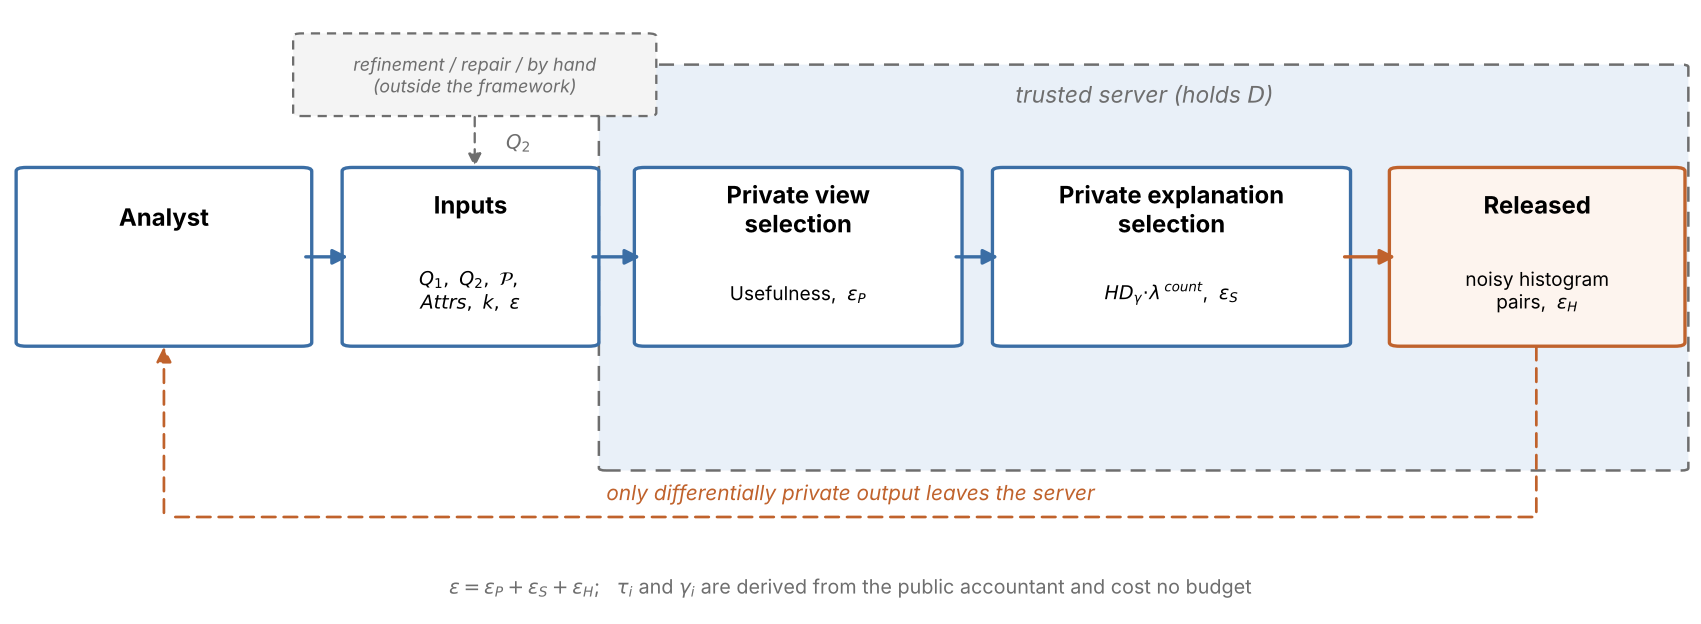
\includegraphics[width=\linewidth]{figures/framework.png}
\caption{The private query-difference explanation framework.
The analyst supplies both queries together with the search space and the budget; where $Q_2$ came from, whether a refinement algorithm, a repair procedure or the analyst, is outside the framework.
The server privately selects views, then explanations, and releases only noisy histogram pairs.
The constants $\tau$ and $\gamma$ are fixed from public quantities and therefore consume no budget.}
\label{fig:framework}
\end{figure*}

\paragraph{The structure of an explanation.}
An explanation answers \emph{where} the two outputs differ and \emph{in what respect}.
The where is a region of the database, given by a view predicate $p\in\views$; the respect is an attribute $A\in\Attrs$, whose distribution the two outputs are compared on.

\begin{definition}[Histogram Explanation Candidate]
\label{def:candidate}
Given a view $p\in\views$ and an explanation attribute $A\in\Attrs$, the \emph{histogram explanation candidate} $e=(p,A)$ induces the two histograms
\[
    \hist{Q_1(\pD)}{A}
    \qquad\text{and}\qquad
    \hist{Q_2(\pD)}{A}.
\]
Writing $\mathrm{attr}(p)$ for the attributes the predicate $p$ constrains, the space of candidates is
\[
\added{\mathcal{E}}=\{(p,A)\in\views\times\Attrs \;:\; A\notin\mathrm{attr}(p)\},
\]
and we write $E\subseteq\mathcal{E}$ for a set of them\added{, and $A_c$ for the attribute of a candidate $c\in\mathcal{E}$}.
\ag{$\mathcal{C}$ already denotes the output-constraint set in Definitions~\ref{def:output-constraint} and~\ref{def:refinement}, both cited earlier in this section. Suggest renaming one of the two, for instance $\mathcal{E}$ for the candidate space here.}
A view that fixes $A$ leaves the two histograms supported on a single bin, so such a pair reports the change in one count rather than a change in a distribution; excluding it also keeps the candidate space aligned with the reference set of Section~\ref{sec:explanation-quality}, from which $\mathrm{attr}(p)$ is excluded for the same reason.
\end{definition}

\begin{example}[Explanation candidates]
\label{ex:candidate}
Figure~\ref{fig:candidates} shows two candidates for the refinement of Example~\ref{ex:running}, both on $A=\texttt{occupation}$.
In panel (a) the view is $p=(\texttt{education}=\texttt{Masters})$: both queries meet it, and the refinement shifts the occupational mix towards professional-specialty roles rather than merely adding people.
In panel (b) the view is $p'=(\texttt{education}=\texttt{Bachelors})$, which $\varphi_2$ cannot satisfy, so $Q_2(p'(D))=\emptyset$ and the candidate reports a population the refinement removes in its entirety.
Neither change is visible in the aggregate value, and the second is the kind of one-sided view the measures of Section~\ref{sec:explanation-quality} have to handle rather than discard.
\end{example}

\begin{figure*}[t]
\centering
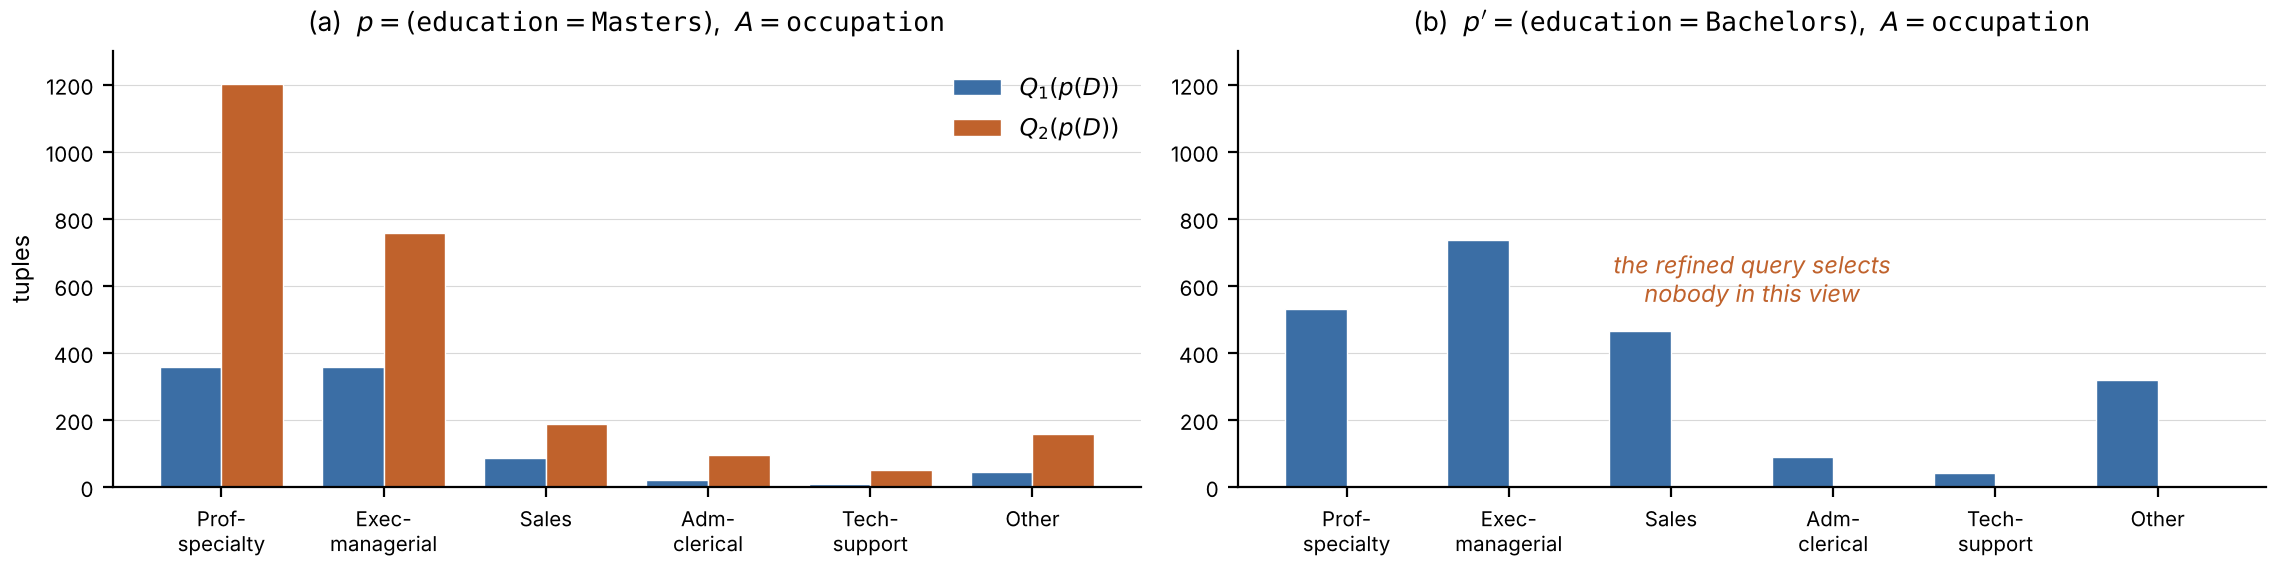
\includegraphics[width=\linewidth]{figures/candidates.png}
\caption{Two explanation candidates on Adult, for $Q_1$ selecting Bachelor's and Master's degree holders working at least $50$ hours and $Q_2$ selecting Master's degree holders working at least $30$ (Example~\ref{ex:candidate}). Counts are exact; what the framework releases is each pair of bars perturbed with Laplace noise.}
\label{fig:candidates}
\end{figure*}

What is released for a selected candidate is a perturbed version of its two histograms, in the sense of the Laplace mechanism (Definition~\ref{def:laplace-mechanism}).

\begin{definition}[Noisy histogram]
\label{def:noisy-histogram}
For a set of tuples $T\subseteq D$, an attribute $A$ and a scale $b>0$, the \emph{noisy histogram} of $A$ over $T$ is
\[
\hat H_{T,A}(v)=\hist{T}{A}(v)+Y_v,\qquad v\in\Dom(D[A]),
\]
with $Y_v$ drawn independently from the Laplace distribution of scale $b$, one draw per bin of the public domain of $A$.
\end{definition}

We release the pair $\big(\hat H_{Q_1(p(D)),A},\hat H_{Q_2(p(D)),A}\big)$ rather than only its difference, so that the analyst sees the two profiles themselves and not just the size of the gap between them.
The pair costs more: a tuple selected by both queries changes both histograms, so the pair has $L_1$-sensitivity $2$ against $1$ for the difference (Proposition~\ref{prop:histogram-release-sensitivity}), which doubles the noise scale at a fixed budget.
Where budget is scarce the difference can be released instead.


\subsection{Measures of Explanation Quality}
\label{sec:explanation-quality}

The criteria we optimise are the four reviewed in Section~\ref{subsec:prelim-quality}: interestingness, representativeness, coverage and diversity.
None is new.
What is new is the form we give them, and the reason for the change is always the same: a measure whose value can be swung by one individual cannot be optimised under differential privacy at all, because the noise a private mechanism must add is calibrated to exactly that swing.
\added{For the three criteria that read the database we therefore recall the form used in prior work, say what goes wrong with it here, and give the form we use; diversity reads only released outputs and needs no such change.}
Section~\ref{subsec:ideal-sensitivity} states the effect of all four changes in one place.

\paragraph{Interestingness.}
In its distributional form a candidate is scored by the distance between the two distributions it induces~\cite{SeeDB,FEDEX}, which in our setting is the total variation distance between the conditional distributions of $A$ over $Q_1(p(D))$ and $Q_2(p(D))$, or twice it in the normalised form.
Two things go wrong.
It is undefined when one of the two outputs does not meet the view, which is exactly the case of the one-sided views of Example~\ref{ex:candidate}, where a refinement adds or removes a population wholesale.
And because it is a ratio over the output sizes, a single tuple can move it by half of its entire range, however large the database (Proposition~\ref{prop:sensitivity-itemized}).
We therefore compare the two outputs \emph{bin by bin in counts}, normalised by the size of the bin in the view rather than by the size of the outputs, and add a public constant $\gamma$ to each denominator.

\begin{definition}[Smoothed Histogram Distance]
\label{def:hd}
Given a dataset $D$, a view predicate $p$, an attribute $A$, two queries $Q_1,Q_2$, and a public smoothing constant $\gamma \ge 0$,
\begin{multline}
\HD_\gamma(D;p,A,Q_1,Q_2) = \\
\sum_{v\in \Dom(D[A])}
\frac{\big|\hist{\Qone(\pD)}{A}(v)-\hist{\Qtwo(\pD)}{A}(v)\big|}
     {\hist{\pD}{A}(v)+\gamma}
\label{eq:hd-definition}
\end{multline}
\end{definition}

Setting $\gamma=0$ recovers the unsmoothed score, in which case the sum must be restricted to bins with $H_{p(D),A}(v)>0$ to avoid division by zero.
For $\gamma>0$ no such restriction is needed: a bin absent from $p(D)$ is necessarily absent from $Q_1(p(D))$ and $Q_2(p(D))$ as well, since both are subsets of $p(D)$, so it contributes exactly $0/\gamma=0$.

The motivation for $\gamma$ is a mismatch between the \emph{worst case} the sensitivity bound must cover and the \emph{typical case} the mechanism actually encounters.
A bin containing two tuples can have its ratio swung by a full unit by a single individual, so the unsmoothed bound must accommodate that; yet the bound is then applied uniformly, including to candidates supported by thousands of tuples.
The exponential mechanism consequently cannot separate candidates whose scores differ by far less than the bound.
Smoothing raises every denominator by a fixed public amount, which barely perturbs well-supported bins while removing the pathological ones from consideration.

The resulting bound is strictly decreasing in $\gamma$, which is the entire point: $\gamma$ buys a tighter worst case at the cost of a mild, uniform compression of every candidate's score.
The same device appears in differentially private decision-tree induction, where split criteria built from ratios of counts are smoothed for this reason~\cite{FriedmanSchuster10}, and in~\cite{DPClustX}, which rescales its cluster-quality measures by the cluster size; Section~\ref{subsec:prelim-dp} contrasts it with calibrating noise to the data instead.

\paragraph{Representativeness.}
Subgroup discovery scores a region by trading its unusualness against its generality~\cite{Wrobel97,HerreraCGJ11}; we need the requirement in the opposite direction, since the deviation we report is the change \emph{inside} a region and the region itself should be typical of the database.
The natural form is $1-\TVD$ between the distribution of an attribute inside the view and in the whole database.
Here too the view-side term $d_v/m$ is a ratio whose denominator is the view size, so a single tuple can rewrite the profile of a near-empty view (Proposition~\ref{prop:sensitivity-itemized}), and the measure is undefined when the view is empty.
\added{That instability is a question of evidence rather than of privacy: Proposition~\ref{prop:usefulness-sensitivity} holds at every $\gamma_R$, the product with coverage absorbing the sensitivity, since $\Cov\le2m/N$ vanishes on exactly the views whose profile is unstable.
But a profile built on a handful of tuples is not worth reading at face value, whatever its sensitivity.}
The same smoothing repairs both.

\begin{definition}[Smoothed Representativeness]
\label{def:rep}
Let $c^A_v$ and $d^A_v$ be the number of tuples with $A$-value $v$ in $D$ and in $p(D)$, let $N=|D|$ and $m=|p(D)|$, and let $\gamma_R\ge0$ be a public constant.
For a single attribute,
\begin{equation}
\Rep^A_{\gamma_R}(p,D)=1-\frac{1}{2}\sum_{v\in\Dom(D[A])}\left|\frac{c^A_v}{N}-\frac{d^A_v}{m+\gamma_R}\right| ,
\label{eq:representativeness-proxy}
\end{equation}
and the representativeness of the view is the average over the reference attributes it does not itself constrain,
\begin{equation}
\Rep_{\gamma_R}(p,D)=\frac{1}{|\mathcal{A}_R(p)|}\sum_{A\in\mathcal{A}_R(p)}\Rep^A_{\gamma_R}(p,D),
\label{eq:rep-average}
\end{equation}
where $\mathcal{A}_R(p)=\mathcal{A}_R\setminus\mathrm{attr}(p)$.
\end{definition}

Two conventions are fixed by Eq.~\eqref{eq:rep-average}.
The reference set $\mathcal{A}_R$ is chosen in advance and does not depend on the candidate attribute, since representativeness is a property of the view and is evaluated before views are paired with attributes.
And the attributes the view itself constrains are excluded, because comparing $p(D)$ with $D$ on the attribute that defines $p$ is close to tautological: a view $\texttt{occupation}=c$ necessarily has an extreme occupation distribution.
We assume $|\mathcal{A}_R|>\ell$, so that $\mathcal{A}_R(p)$ is never empty.

\added{How large should $\gamma_R$ be?
Of the mass Eq.~\eqref{eq:representativeness-proxy} weighs against $D$, the view supplies
$m/(m+\gamma_R)$ and the smoothing the rest; since the smoothing part copies the profile of $D$
itself, that ratio is the \emph{fidelity} at which the view is read.
Proposition~\ref{prop:rep-range} prices it: the values $\Rep_{\gamma_R}$ can take span an interval
of length $\tfrac{m}{m+\gamma_R}\big(1-\tfrac{m+\gamma_R}{N}\big)$, which closes to a point once
$m+\gamma_R\ge N$ --- at $\gamma_R=N$, for every view at once, leaving the reference attributes
unread. We set instead
\begin{equation}
\gamma_R=\alpha N,\qquad \alpha=\tfrac{1}{100},
\label{eq:gammaR-rule}
\end{equation}
reading a view at fidelity $\tfrac12$ once it holds an $\alpha$ fraction of $D$ and damping
smaller ones, which is what smoothing is for; on Adult that is a few hundred tuples.
Section~\ref{subsec:two-stages} balances $\gamma$ the same way, against the support of a single
bin rather than of the whole view (Remark~\ref{rem:gamma-window}).
Both $\alpha$ and $N$ are public (Section~\ref{subsec:prelim-db-queries}), so the choice costs no
budget and $\gamma_R$ is a constant of the mechanism rather than an argument of
Algorithm~\ref{alg:main}.}

\begin{proposition}[Range of smoothed representativeness]
\label{prop:rep-range}
\added{Fix a database size $N$, a view size $m\le N$ and a reference attribute $A$, and write
$M=m+\gamma_R$. As the two $A$-profiles range over all non-negative vectors $(c^A_v)_v$ and
$(d^A_v)_v$ with $\sum_v c^A_v=N$, $\sum_v d^A_v=m$ and $d^A_v\le c^A_v$, the values of
$\Rep^A_{\gamma_R}$ fill an interval of length
\[
\frac{m}{M}\Big(1-\frac{M}{N}\Big)\quad\text{if }M<N,\qquad\text{and a single point otherwise.}
\]
So do the values of $\Rep_{\gamma_R}$, which averages such quantities over attributes whose
profiles may be chosen independently of one another.}
\end{proposition}

\begin{proof}
\added{Write $x_v=c^A_v/N$ and $y_v=d^A_v/M$, so $\sum_v x_v=1$ and $\sum_v y_v=m/M$, and put
\[
S=\sum_v\min(x_v,y_v) .
\]
Since $\sum_v|x_v-y_v|=\sum_v x_v+\sum_v y_v-2S$, Eq.~\eqref{eq:representativeness-proxy} reads
\[
\Rep^A_{\gamma_R}=\frac{1-m/M}{2}+S ,
\]
an increasing affine function of $S$. The admissible pairs form a convex set and $S$ is
continuous on it, so both range over an interval of the same length, and it is enough to find the
two ends of the overlap $S$.

\emph{Above.} $\min(x_v,y_v)\le y_v$ gives $S\le m/M$, with equality exactly when $y_v\le x_v$ for
every $v$. A view drawn in proportion to the database, $d^A_v=m\,c^A_v/N$, has
$y_v=(m/M)\,x_v\le x_v$ and attains it.

\emph{Below.} From $d^A_v\le c^A_v$ we get $y_v\le c^A_v/M=(N/M)\,x_v$, so $x_v\ge(M/N)\,y_v$; and
$y_v\ge(M/N)\,y_v$ whenever $M\le N$. Hence $\min(x_v,y_v)\ge(M/N)\,y_v$ for every $v$, and
summing, $S\ge(M/N)(m/M)=m/N$. A view sitting on a single value attains it: let one value occur
exactly $m$ times in $D$ with all of its tuples inside the view, so that
$S=\min(m/N,\,m/M)=m/N$.

So $S$ fills $[m/N,\,m/M]$, an interval of length $\tfrac{m}{M}-\tfrac{m}{N}=\tfrac mM(1-\tfrac MN)$.
If instead $M\ge N$ then $y_v\le c^A_v/M\le c^A_v/N=x_v$ for every $v$, so $S=m/M$ always and the
interval is a point.}
\end{proof}
Smoothing has a second, useful consequence: it bounds $\Rep_{\gamma_R}$ away from $1$, which the proof of Proposition~\ref{prop:usefulness-sensitivity} relies on.
The two vectors compared in Eq.~\eqref{eq:representativeness-proxy} do not carry the same total mass: the database side sums to $1$, while the view side sums to $m/(m+\gamma_R)$, which is below $1$ because smoothing inflates the denominator without adding to the counts.
Two non-negative vectors are at least as far apart in $L_1$ as their totals differ, so whatever the two profiles look like,
\[
\sum_v\Big|\tfrac{c_v}{N}-\tfrac{d_v}{m+\gamma_R}\Big|\;\ge\;1-\frac{m}{m+\gamma_R}\;=\;\frac{\gamma_R}{m+\gamma_R},
\]
and substituting this into Eq.~\eqref{eq:representativeness-proxy} gives
\begin{equation}
\Rep_{\gamma_R}(p,D)\;\le\;1-\frac{\gamma_R}{2(m+\gamma_R)}\;\added{\overset{\gamma_R=\alpha N}{\le}\;\frac{2+\alpha}{2(1+\alpha)}},
\label{eq:rep-upper}
\end{equation}
\added{for the last step, $m\le N$ makes $m+\gamma_R\le(1+\alpha)N$, so the fraction is at least $\alpha/(2(1+\alpha))$}, and the average inherits the bound from the attributes it averages.
It is attained when the view is the whole database, and it is the upper end of the interval of Proposition~\ref{prop:rep-range}.


\paragraph{Coverage.}
A deviation seen on a handful of tuples is not evidence, and explanation frameworks pair a deviation measure with a mass measure: the support of association rules~\cite{AgrawalIS93}, the support threshold of MacroBase~\cite{MacroBase} and of \textsc{Diff}~\cite{DIFF}, the coverage of an anchor~\cite{Anchors}.
Since the object being explained is a comparison, the mass has to account for both outputs.
Taking the product of the two output sizes, as a two-sided support measure suggests, has the same defect as the distributional interestingness: it vanishes on one-sided views, and \added{it grows with the two output sizes}, which is what makes a single tuple move it by an amount that grows with $N$ (Proposition~\ref{prop:sensitivity-itemized}).
\ag{Small issue: The sensitivity of the product is $o_1+o_2+1$, so it grows with the two output sizes, and the view size enters only as an upper bound on them. Saying it grows with the outputs would be more accurate.}
We take instead the evidence the two outputs place in the view \emph{jointly}, normalised by the public $N$:

\begin{equation}
\Cov(p,Q_1,Q_2,D)=\frac{|Q_1(p(D))|+|Q_2(p(D))|}{|D|}.
\label{eq:coverage-proxy}
\end{equation}
Dividing by $N$ costs nothing, since $N$ is public (Section~\ref{subsec:prelim-db-queries}), and it removes the growth with the database size: $\Cov$ reads as a fraction of the database rather than a count, so it is comparable across datasets and across views of very different sizes.
Its range is $[0,2]$, the upper end reached only when both outputs cover all of $D$, and it is $0$ exactly when neither output meets the view, which is the one case in which there is nothing to explain.
Summing rather than taking the smaller of the two counts matters for the same reason the sum replaces the product: a view that one output fills and the other leaves empty keeps the full weight of the evidence that is there.

\paragraph{Diversity.}
When several results are returned together their marginal value depends on what has already been shown, which is the principle of maximal marginal relevance~\cite{MMR} and of the axiomatic treatments that follow it~\cite{GollapudiS09,LinBilmes11}.
The aspect an explanation describes is its attribute, so we discourage reusing one, and grade the penalty by how many times it has already been used rather than charging every repeat alike:
\begin{equation}
\DivS(A,S)=\lambda^{\,\mathrm{count}(A,S)},
\qquad 0\le\lambda\le1,
\label{eq:diversity-score}
\end{equation}
where $\mathrm{count}(A,S)$ is the number of previously selected explanations already using attribute~$A$.
At $\lambda=1$ the term disappears and repeats are free; at $\lambda=0$ every repeat scores zero, which empties a candidate of value without removing it from the pool, so the mechanism may still return one.
Since $\DivS$ reads only previously selected \emph{outputs} and never the database, it adds no data sensitivity to the selection utility.

\paragraph{From a sequence to a set.}
Equation~\eqref{eq:diversity-score} is defined relative to the explanations chosen in earlier iterations, so as written it scores an \emph{ordered sequence}, not a set, while what we release is a set.
We therefore state the objective the algorithm approximates directly.

\begin{definition}[Set-level explanation utility]
\label{def:setobj}
Let $E$ be a set of candidates, and for an attribute $A$ let
$h^A_{(1)}\ge h^A_{(2)}\ge\cdots$ be the scores $\HD_\gamma(c)$ of the members of $E$ with $A_c=A$, in decreasing order\added{, with $h^A_{(j)}=0$ for every $j$ beyond the size of that group}.
For a non-increasing weight profile $w_1\ge w_2\ge\cdots\ge0$ with $w_1=1$,
\begin{equation}
F_w(E)=\sum_{A}\;\sum_{j\ge1} w_j\, h^A_{(j)} .
\label{eq:set-objective}
\end{equation}
\end{definition}
\ag{$A_c$ has not been introduced. Adding one clause to Definition~\ref{def:candidate}, writing $A_c$ for the attribute of a candidate $c$, fixes it here and in Proposition~\ref{prop:setobj}.}
\ag{The inner sum of Eq.~\eqref{eq:set-objective} has no upper limit, while $h^A_{(j)}$ exists only up to the size of the attribute group. Simplest fix is to adopt the convention $h^A_{(j)}=0$ for $j$ beyond the group.}

Within each attribute group the strongest explanation counts in full and every further one is discounted by its rank.
The graded penalty of Equation~\eqref{eq:diversity-score} is the profile $w_j=\lambda^{\,j-1}$, and a flat rule is $w=(1,\lambda,\lambda,\dots)$.
The two agree on the first two members of a group and differ only from the third onwards, so they can disagree about which set is best only when some attribute is used at least three times: that needs $k\ge3$, and once $k>2|\Attrs|$ it is unavoidable.

\begin{proposition}[The set objective agrees with the sequential rule]
\label{prop:setobj}
Order $E$ arbitrarily and write $S_{<c}$ for the members preceding $c$, so that the per-round rule of Eq.~\eqref{eq:diversity-score} awards $E$ the total $\sum_{c\in E}\HD_\gamma(c)\cdot\DivS(A_c,S_{<c})$.
With $w_j=\lambda^{\,j-1}$, $F_w(E)$ equals that total under the ordering maximising it, and upper-bounds it under every ordering.
\end{proposition}

\begin{proof}
Since $\mathrm{count}(A,S)$ counts only the members of $S$ that carry $A$, the weight a candidate receives depends on its position within its own attribute group and not on how the groups are interleaved.
The total therefore splits into independent per-group totals, and an ordering is free to choose each group's internal order.
Within the group of $A$, an ordering that places a member $j$-th awards it $\lambda^{\,j-1}$, so the group total is $\sum_j \lambda^{\,j-1}h_{\sigma(j)}$ for the induced permutation $\sigma$.
The weights are non-increasing, so by the rearrangement inequality this is maximised by pairing the largest weight with the largest score, that is by visiting the group in decreasing $\HD_\gamma$, and the maximum is $\sum_j \lambda^{\,j-1}h^A_{(j)}$.
Summing over groups gives Eq.~\eqref{eq:set-objective}, and no ordering gives more.
The special cases $\lambda=0$ and $\lambda=1$ recover a group maximum and a modular sum respectively.
\end{proof}


\added{Greedy selection on $F_w$ is not a constant-factor approximation. Because $F_w$ decomposes over attribute groups with no interaction between them, it returns the \emph{exact} maximiser, and the per-round score of Algorithm~\ref{alg:topk} is precisely its marginal gain; Appendix~\ref{app:greedy} establishes both.}
\ag{The $(1-1/e)$ guarantee requires $F_w$ to be monotone submodular, which is now proved only in the appendix, so the reader meets the guarantee before the hypothesis. Please add one sentence recording that $F_w$ is monotone submodular, with a pointer to the appendix, closes the gap.}

\subsection{Sensitivity of the Measures}
\label{subsec:ideal-sensitivity}

Private selection with the exponential mechanism (Definition~\ref{def:exponential-mechanism}) calibrates its randomness to the global sensitivity of the utility (Definition~\ref{def:global-sensitivity}).
All statements are with respect to the unbounded neighbouring relation of Definition~\ref{def:neighboring}.
For a function $f$ and a size $N$ we write $\GS_N(f)$ for the largest change of $f$ between a database of size $N$ and a neighbour, so that $\GS(f)=\sup_N\GS_N(f)$.
\added{Under Definition~\ref{def:neighboring} a neighbour of a database of size $N$ has size $N+1$ or $N-1$, and that asymmetry is what the two cases of Proposition~\ref{prop:usefulness-sensitivity} turn on.}
\ag{This sentence is dense. Two things would help. The clause after the semicolon repeats what the supremum already says and can go. And it is worth stating that a neighbour of a database of size $N$ has size $N+1$ or $N-1$, since that asymmetry is exactly what the two cases of Proposition~\ref{prop:usefulness-sensitivity} turn on.}
\added{A mechanism running on the private database cannot read its scale off $|D|$. Under Definition~\ref{def:neighboring} a neighbouring pair has $|D|=N$ and $|D'|=N+1$, so such a mechanism would run at two different scales on the two databases, whereas the $e^{\epsilon}$ argument needs one scale common to both. It must instead fix the scale from a public $\bar N$ that does not depend on $D$ and satisfies $\bar N\le|D|$, which is what Section~\ref{sec:solution} does; the bounded relation, under which the size is constant across the pair, would serve equally well.}
\ag{Publicity of $|D|$ is necessary here but it is not sufficient. Under Definition~\ref{def:neighboring} a neighbouring pair has $|D|=N$ and $|D'|=N+1$, so a mechanism that takes its scale from $|D|$ runs the exponential mechanism at two different temperatures on the two databases, whereas the usual $e^{\epsilon}$ argument needs one common scale. Two possible fixes. Either adopt the bounded relation, where $N$ is genuinely constant across the pair, or fix the scale from a public $\bar N$ that does not depend on $D$.}
Upper bounds below hold for every candidate; lower bounds and equalities are attained by explicit databases, and so require that the view and the two queries admit the tuples those databases use.
We begin with the one bound that takes real work, the smoothed Histogram Distance, and then state all four results together.

\begin{proposition}[Sensitivity of Smoothed Histogram Distance]
\label{prop:hd-sensitivity}
$\GS(\HD_\gamma)=\dfrac{1}{1+\gamma}$.
\end{proposition}

\begin{proof}
Let $D'=D\cup\{t\}$.
If $t$ does not satisfy $p$ nothing changes.
Otherwise $t$ falls into exactly one bin $v^*$ of $A$, and every other term of Eq.~\eqref{eq:hd-definition} is unchanged, so only that term has to be bounded.
Write $n=\hist{\pD}{A}(v^*)$ for the support of the view in that bin and $q_j=\hist{Q_j(\pD)}{A}(v^*)$ for $j=1,2$ for the two output counts in it, and let $n'=\hist{p(D')}{A}(v^*)$ and $q_j'=\hist{Q_j(p(D'))}{A}(v^*)$ be the same quantities on $D'$.
The numerators of the term before and after are $x=|q_1-q_2|$ and $x'=|q_1'-q_2'|$; since $Q_j(\pD)\subseteq\pD$ by Proposition~\ref{prop:view-restriction}, $0\le x\le n$.
Each query either selects $t$ or not, so $q_j'=q_j+\delta_j$ with $\delta_j\in\{0,1\}$, and $n'=n+1$ because $t$ satisfies $p$ and falls in $v^*$.
Substituting these,
\[
x'=|q_1'-q_2'|=\big|(q_1+\delta_1)-(q_2+\delta_2)\big|=\big|(q_1-q_2)+(\delta_1-\delta_2)\big| ,
\]
whereas $x=|q_1-q_2|$.
Both $x$ and $x'$ are absolute values, so by the reverse triangle inequality their difference is at most the absolute value of the difference of their arguments:
\[
|x'-x|\;\le\;\big|\,[(q_1-q_2)+(\delta_1-\delta_2)]-(q_1-q_2)\,\big|\;=\;|\delta_1-\delta_2|\;\le\;1 ,
\]
the last step because $\delta_1,\delta_2\in\{0,1\}$.
The term therefore moves from $x/(n+\gamma)$ to $x'/(n+1+\gamma)$.
\added{If $n=\gamma=0$ the bin is excluded from the sum on $D$ by the restriction stated after Definition~\ref{def:hd} and present in it on $D'$, so the comparison is between an absent term and one of value $x'\le1=\frac{1}{1+\gamma}$.}
\ag{One sentence here: At $\gamma=0$ this bin is excluded from the sum on $D$ by the restriction stated after Definition~\ref{def:hd} and included on $D'$, so the comparison is between a term that is absent and a term that is present. As written it reads as though the bin sat in both sums.}
Otherwise put $K=(n+\gamma)(n+1+\gamma)>0$ and bound the two directions separately.
Upwards, using in turn $x'\le x+1$, a common denominator, the cancellation of $xn+x\gamma$, then $x\ge0$ and $n\ge0$:
\begin{align*}
\frac{x'}{n+1+\gamma}-\frac{x}{n+\gamma}
&\;\le\;\frac{x+1}{n+1+\gamma}-\frac{x}{n+\gamma}\\[2pt]
&\;=\;\frac{(x+1)(n+\gamma)-x(n+1+\gamma)}{K}\\[2pt]
&\;=\;\frac{n+\gamma-x}{K}\\[2pt]
&\;\le\;\frac{n+\gamma}{K}\;=\;\frac{1}{n+1+\gamma}\\[2pt]
&\;\le\;\frac{1}{1+\gamma}.
\end{align*}
Downwards, using in turn $x'\ge x-1$, a common denominator, the same cancellation, then $x\le n$ and the step $(\star)$ below:
\begin{align*}
\frac{x}{n+\gamma}-\frac{x'}{n+1+\gamma}
&\;\le\;\frac{x}{n+\gamma}-\frac{x-1}{n+1+\gamma}\\[2pt]
&\;=\;\frac{x(n+1+\gamma)-(x-1)(n+\gamma)}{K}\\[2pt]
&\;=\;\frac{x+n+\gamma}{K}\\[2pt]
&\;\le\;\frac{2n+\gamma}{K}\\[2pt]
&\;\overset{(\star)}{\le}\;\frac{1}{1+\gamma}.
\end{align*}
Step $(\star)$ is the only one that is not immediate.
It asserts $(2n+\gamma)/K\le 1/(1+\gamma)$.
Since $K>0$ and $1+\gamma>0$, cross-multiplying preserves the inequality, so the claim is equivalent to $K-(2n+\gamma)(1+\gamma)\ge0$.
Expanding both products,
\begin{align*}
(2n+\gamma)(1+\gamma)&=2n+2n\gamma+\gamma+\gamma^2,\\[2pt]
K=(n+\gamma)(n+1+\gamma)&=n^2+n+2n\gamma+\gamma+\gamma^2 .
\end{align*}
The terms $2n\gamma+\gamma+\gamma^2$ occur in both lines and cancel, leaving $n^2+n$ from the second and $2n$ from the first, so
\[
K-(2n+\gamma)(1+\gamma)=(n^2+n)-2n=n(n-1),
\]
which is non-negative for every integer $n\ge0$, vanishing only at $n=0$ and $n=1$.
Equality holds for a bin holding one tuple of the view selected by $Q_1$ only, whose term is $\frac{1}{1+\gamma}$: adding a tuple of the same bin selected by $Q_2$ only makes the two counts equal and the term $0$.
\end{proof}

Step $(\star)$ is an equality exactly when $n(n-1)=0$, that is for $n\in\{0,1\}$: a bin the new tuple populates from empty, or one already holding a single tuple of the view.
For $n\ge2$ the bound $(2n+\gamma)/\big((n+\gamma)(n+1+\gamma)\big)$ is strictly smaller, and it falls as $n$ grows.
The sensitivity is therefore dictated by the sparsest bins of any view, whereas the candidates that make good explanations rest on well-populated ones.


\begin{proposition}[Sensitivity of the forms used in prior work]
\label{prop:sensitivity-itemized}
Let $N$ be the database size, and restrict attention to neighbouring databases on which the measure in question is defined.
\begin{enumerate}[label=(\roman*),leftmargin=*]
\item \emph{Interestingness.} The distributional form has $\GS\ge1$, half of its range $[0,2]$.
\item \emph{Representativeness.} The unsmoothed form $1-\TVD$ has $\GS_N\ge\frac12-\frac1N$.
\item \emph{Coverage.} The two-sided support $|Q_1(\pD)|\,|Q_2(\pD)|$ has $\GS_N=2N+1$.
\end{enumerate}
None of the three decays with $N$, and the last grows with it.
\end{proposition}

\begin{proof}
(i) The score is twice a total variation distance and so lies in $[0,2]$.
Let $Q_1(\pD)=\{t\}$ with $t[A]=v_1$, and let $Q_2(\pD)$ place all its mass on a bin $v_2\ne v_1$, so the two conditional distributions are point masses at $v_1$ and at $v_2$ and the score is $2$.
Add one tuple of the view, selected by $Q_1$ only and with $A$-value $v_2$: the first distribution becomes uniform on $\{v_1,v_2\}$ and the score drops to $1$.
The rest of $D$ is unconstrained, so a change of $1$ is available at every database size.

(ii) Let $D$ hold one tuple of the view carrying the value $v_1$ on every attribute of $\mathcal{A}_R(p)$, together with $N-1$ tuples outside the view carrying $v_2$.
The view distribution is then a point mass at $v_1$ while the database gives $v_1$ weight $\tfrac1N$, so the measure is $\tfrac1N$.
Adding one tuple of the view with value $v_2$ makes the view distribution uniform on $\{v_1,v_2\}$ and the measure $\tfrac{N+3}{2(N+1)}$.
The change is $\tfrac{N+3}{2(N+1)}-\tfrac1N$, which exceeds $\tfrac12-\tfrac1N$ because $\tfrac{N+3}{2(N+1)}>\tfrac12$.

(iii) Write $o_j=|Q_j(\pD)|$ for $j=1,2$; by Proposition~\ref{prop:view-restriction} both are at most $m=|\pD|\le N$.
A tuple of the view selected by both queries sends $o_1o_2$ to $(o_1+1)(o_2+1)$, a change of
\[
(o_1+1)(o_2+1)-o_1o_2=o_1+o_2+1\;\le\;2N+1 .
\]
Equality holds at $o_1=o_2=m=N$, that is when the view is the whole database and both queries select all of it.
\end{proof}

\subsection{The Two-Stage Model}
\label{subsec:two-stages}

A single private selection over $\mathcal{E}$ would have to score every candidate, and scoring a candidate means building the histograms of its attribute over both outputs inside its view.
That is $|\views|\cdot|\Attrs|$ pieces of work, repeated in each of the $k$ selection rounds.
Most of it is wasted: representativeness and coverage depend on the view alone, so whether a region can support an explanation at all can be decided before any attribute is looked at.
The framework therefore splits the problem in two.
The \emph{view stage} scores each view by the product of the two region-level measures,
\begin{equation}
\Use(p,Q_1,Q_2,D)= \Rep_{\gamma_R}(p,D)\cdot \Cov(p,Q_1,Q_2,D),
\label{eq:usefulness-proxy}
\end{equation}
with $\Rep_{\gamma_R}$ from Definition~\ref{def:rep} and $\Cov$ from Eq.~\eqref{eq:coverage-proxy}, and retains the $\tau$ best.
The \emph{explanation stage} then scores only the candidates built from the retained views, by the product of the two candidate-level measures:
\begin{equation}
\widetilde{U}_i(D;c)=\HD_{\gamma}(D;p,A,Q_1,Q_2)\cdot \DivS(A,S_{i-1})
\label{eq:selection-utility}
\end{equation}
for a candidate $c=(p,A)$.
\ag{The workflow paragraph and Figure~\ref{fig:framework} say $\gamma$ is refreshed each round from the accountant, so this utility and Proposition~\ref{prop:selection-utility-sensitivity} are really stated for the round's $\gamma_i$. Suggest carrying the index here, or adding a clause that the bound holds for whichever $\gamma$ the round uses.}
This reduces the candidate-level work from $|\views|\cdot|\Attrs|$ to $\tau\cdot|\Attrs|$, a factor $|\views|/\tau$, in every round.

Efficiency is the visible reason for the split, but not the binding one.
A single-stage mechanism would have to select on the product of all four measures, and a product is worse than its factors: by the product rule its sensitivity picks up a term in which the movement of one factor is multiplied by the \emph{level} of the other, and the levels here are not small.
Coverage alone can reach $2$, so an interestingness score that moves by $\Delta$ drags the combined score by $2\Delta$ before the coverage term is even counted.
Splitting removes that cross term entirely.
Each stage is its own private mechanism, calibrated to the sensitivity of its own utility, and neither pays for the other's range.
Propositions~\ref{prop:usefulness-sensitivity} and~\ref{prop:selection-utility-sensitivity} are what the two stages pay, and Section~\ref{subsec:dp-proof} composes them into $\epsilon$.
\begin{proposition}[Sensitivity of View Usefulness]
\label{prop:usefulness-sensitivity}
\added{Let $\gamma_R=\alpha N$ for a public $\alpha\in[0,1]$, as in Eq.~\eqref{eq:gammaR-rule}.
Then
\[ \GS_N(\Use)\;\le\;\frac{4}{N}. \]}
\end{proposition}

\begin{proof}
\added{Write $m=|\pD|$ for the view size, $M=m+\gamma_R$ for the smoothed view size, and
$s=|Q_1(\pD)|+|Q_2(\pD)|$ for the evidence the two outputs place in the view, so that
$0\le s\le2m\le2N$ by Proposition~\ref{prop:view-restriction} and $\Cov=s/N$.
For a reference attribute $A$ let $x^A_v=c^A_v/N$ and $y^A_v=d^A_v/M$ be the two profiles it
compares, and write $\theta=\sum_v y^A_v=m/M$, the same for every $A$.
A prime marks a quantity on a neighbour of size $N+1$, and $\Delta$ a primed quantity minus its
unprimed one.
We bound the change to such a neighbour first and collect the two directions at the end.
So let $D'=D\cup\{t\}$, let $v(t)$ be the $A$-value of $t$, and set
\[
w^A=\Delta y^A-\Delta x^A ,
\]
the relative movement of the two profiles.

\emph{Step 1: the two factors.}
Since $\Use=\Rep_{\gamma_R}\cdot\Cov$ and
$\Delta(\Rep_{\gamma_R}\Cov)=\Cov\,\Delta\Rep_{\gamma_R}+\Rep'_{\gamma_R}\Delta\Cov$,
\begin{equation}
|\Delta\Use|\;\le\;\Cov\,|\Delta\Rep_{\gamma_R}|+\Rep'_{\gamma_R}\,|\Delta\Cov| .
\label{eq:use-split}
\end{equation}

\emph{Step 2: representativeness moves no more than the profiles do.}
By Eq.~\eqref{eq:representativeness-proxy}, $\Rep^A_{\gamma_R}=1-\tfrac12\|x^A-y^A\|_1$, so the
reverse triangle inequality for the $L_1$ norm gives
\begin{align*}
|\Delta\Rep^A_{\gamma_R}|&=\tfrac12\Big|\,\|x'^A-y'^A\|_1-\|x^A-y^A\|_1\Big|\\
&\le\;\tfrac12\big\|(x'^A-y'^A)-(x^A-y^A)\big\|_1\;=\;\tfrac12\|w^A\|_1 .
\end{align*}
What matters is that $w^A$ stays whole: when the view mirrors the database the arrival of $t$
rescales both profiles in step and $w^A$ nearly cancels, which bounding $\|\Delta y^A\|_1$ and
$\|\Delta x^A\|_1$ apart would hide.

\emph{Step 3: how the profiles move.}
Both cases are one computation.
Write $\Lambda=M'-M\ge0$ for the growth of the smoothed view size and
\[
\kappa=\frac{\Lambda\,(N+1)}{M'} .
\]
Away from $v(t)$ neither count changes and only the denominators move, which gives
\[
w^A_v=\frac{c^A_v}{N(N+1)}-\frac{d^A_v\Lambda}{MM'}=\frac{x^A_v-\kappa\,y^A_v}{N+1} .
\]
At $v=v(t)$ the arrival of $t$ adds a further $\rho$ to this, where
\[
\rho=\begin{cases}-1/(N+1), & t\text{ outside the view},\\[2pt]
1/M'-1/(N+1), & t\text{ inside}.\end{cases}
\]
Both $\kappa$ and $\rho$ are the same for every $A$.
Since $x^A$ and $y^A$ are non-negative with $\sum_v x^A_v=1$ and $\sum_v y^A_v=\theta$, we have
$\sum_v|x^A_v-\kappa y^A_v|\le\sum_v x^A_v+\kappa\sum_v y^A_v=1+\kappa\theta$, so summing the two
displays over $v$ and averaging over $\mathcal{A}_R(p)$,
\begin{equation}
|\Delta\Rep_{\gamma_R}|\;\le\;\tfrac12\|w\|_1\;\le\;\frac{1+\kappa\theta}{2(N+1)}+\frac{|\rho|}{2} ,
\label{eq:w-move}
\end{equation}
where $\|w\|_1$ denotes the average of $\|w^A\|_1$ over $\mathcal{A}_R(p)$.
Recall also $\Cov\le2m/N$ and $\Rep'_{\gamma_R}\le\frac{2+\alpha}{2(1+\alpha)}$ from
Eq.~\eqref{eq:rep-upper}.

\emph{Step 4: $t$ falls outside the view.}
Then $m$, $s$ and every $d^A_v$ stay put, $\Lambda=\alpha$ and $M'=M+\alpha$, while
$|\rho|=1/(N+1)$ and $\Delta\Cov=-s/(N(N+1))$ gives $|\Delta\Cov|\le2m/(N(N+1))$.
Putting these into Eqs.~\eqref{eq:w-move} and~\eqref{eq:use-split} and collecting over the common
factor $m/(N(N+1))$, which uses $2+\tfrac{2+\alpha}{1+\alpha}=\tfrac{4+3\alpha}{1+\alpha}$,
\[
|\Delta\Use|\;\le\;\frac{m}{N(N+1)}\cdot\frac{4+3\alpha}{1+\alpha}\;+\;\frac{\alpha\,m^2}{N\,M\,M'},
\]
the second term being $\Cov\cdot\kappa\theta/\big(2(N+1)\big)$ written out.
Both increase in $m$, so both are largest at $m=N$, where the view is all of $D$:
\[
|\Delta\Use|\;\le\;\frac{4+3\alpha}{(1+\alpha)(N+1)}
+\frac{\alpha}{(1+\alpha)\big(N(1+\alpha)+\alpha\big)} .
\]
Subtracting this from $4/N$ leaves
\[
\frac{4}{N(N+1)}+\frac{\alpha\big[\alpha(N+1)-1\big]}
{(1+\alpha)(N+1)\big(N(1+\alpha)+\alpha\big)} ,
\]
and the second term is at least $-1/\big(N(N+1)\big)$, since $\alpha\le1$ and
$N(1+\alpha)+\alpha\ge N$. The difference is therefore at least $3/\big(N(N+1)\big)>0$.

\emph{Step 5: $t$ falls inside the view.}
Now $m$ becomes $m+1$ and $d^A_{v(t)}$ becomes $d^A_{v(t)}+1$, while $s$ becomes $s+\delta$ with
$\delta\in\{0,1,2\}$.
The range of $\delta$ is the number of the two queries that select $t$: an output is
$\sigma_\varphi(D)$ (Section~\ref{subsec:prelim-db-queries}), decided tuple by tuple, so $t$
cannot change whether any other tuple is selected.
Here $\Lambda=1+\alpha$ and $|\rho|=|1/M'-1/(N+1)|$, while $|\Delta\Cov|=|\delta N-s|/(N(N+1))$
is at most $\max(2N-s,\,s)/(N(N+1))$, which ties it to $\Cov=s/N$ rather than letting both reach
their extremes at once.
Writing $\beta=m/N$, Eqs.~\eqref{eq:w-move} and~\eqref{eq:use-split} are again explicit in
$\beta$ and $\Cov$, and the maximum of $(N+1)|\Delta\Use|$ over $\beta\in[0,1]$ and
$\Cov\in[0,2\beta]$ is $3.99$ at
$\alpha=\tfrac1{100}$ and $3.95$ at $\alpha=\tfrac1{20}$.
It rises as $\alpha$ falls, approaching $4$ without reaching it.

\emph{Step 6: the two directions.}
A neighbour of a database of size $N$ has size $N+1$ or $N-1$.
Steps 4 and 5 bound the change to a size-$(N+1)$ neighbour by $4/(N+1)$.
Run at base size $N-1$ they bound the change to a size-$(N-1)$ neighbour by $4/N$: the
computation is unchanged, because $\gamma_R=\alpha n$ leaves $\alpha$ fixed as the base size $n$
varies, and every bound above carries $n+1$ in its denominator.
The second is the larger of the two, and it is what fixes the constant.}
\end{proof}


\begin{proposition}[Sensitivity of the selection utility]
\label{prop:selection-utility-sensitivity}
$\GS(\widetilde{U}_i)\le 1/(1+\gamma)$.
\end{proposition}

\begin{proof}
Condition on the history $S_{i-1}$ of previously released outputs, which is legitimate under adaptive composition.
Given that history, $\DivS(A,S_{i-1})$ is a constant in $[0,1]$ determined entirely by released values, so it acts as a bounded multiplier on the data-dependent factor and cannot increase its sensitivity.
The claim follows from Proposition~\ref{prop:hd-sensitivity}.
\end{proof}

Filtering is not free.
The view stage ranks by $\Use$, which no explanation score enters, so a view of middling usefulness may host the single most interesting explanation and still be dropped; and because the filter itself is private, the retained set is not even the exact top-$\tau$ by $\Use$.
We do not bound what this costs.
The one-shot top-$\tau$ mechanism admits a high-probability utility guarantee whose slack grows as $\tau\Delta\log|\views|/\epsilon_P$, which at $\added{\Delta=4/N}$ is $\added{4\tau\log|\views|/(N\epsilon_P)}$ and so vanishes with the database size.
What that slack must be compared against, however, is not the scale of $\Use$ but the gap between the $\tau$-th and the $(\tau{+}1)$-th best view, and that gap narrows as the view space grows denser.
The guarantee is therefore informative only under a lower bound on the gap, which we do not assume.
What the form does say is that the cost of filtering grows linearly in $\tau$, which is an argument for keeping $\tau$ small.



% Guard: macros.tex is \input both by main.tex (after the packages it needs,
% e.g. amsmath for \DeclareMathOperator) and by individual section files so
% they remain compilable on their own. Loading it twice would redefine every
% \newcommand and abort, so the second and later loads are no-ops.
\ifdefined\PQRmacrosloaded\endinput\fi
\let\PQRmacrosloaded\relax

% --- 0. revision marking ---
% Text added to Section 2 during the current revision is wrapped in \added{...}
% so the advisors can see at a glance what is new. Redefine to \relax to print
% the paper without the marking.
\newcommand{\added}[1]{\textcolor{blue}{#1}}
\long\def\added#1{\begingroup\color{blue}#1\endgroup}  % \long: may span paragraphs


% --- A. operator-style score and function names ---
\newcommand{\HD}{\mathit{HD}}                        % histogram distance; use \HD_\gamma
\newcommand{\Attr}{\mathit{Attr}}                    % attribute set of a schema
\newcommand{\Attrs}{\mathit{Attrs}}                  % attribute set argument
% Abbreviated in MATH only; the prose still spells the names out in full.
% Spelling them out inside formulas makes displayed equations far too wide
% for a two-column layout (the product-rule step below overflowed by 200pt).
\newcommand{\Use}{\mathit{Use}}
\newcommand{\Cov}{\mathit{Cov}}
\newcommand{\Rep}{\mathit{Rep}}
\newcommand{\DivS}{\mathit{Div}}
\newcommand{\TVD}{\mathit{TVD}}
\newcommand{\GS}{\mathit{GS}}                        % global sensitivity
\DeclareMathOperator{\Dom}{Dom}
\DeclareMathOperator{\Lap}{Laplace}

% --- B. core objects ---
\newcommand{\Qone}{Q_1}
\newcommand{\Qtwo}{Q_2}
\newcommand{\pD}{p(D)}
\newcommand{\views}{\mathcal{P}}
\newcommand{\hist}[2]{H_{#1,#2}}                     % \hist{\Qone(\pD)}{A}
\newcommand{\dhist}{\Delta H}
\newcommand{\nhist}{\widetilde{\Delta H}}            % the released noisy object

% --- C. privacy budget and parameters ---
\newcommand{\eps}{\epsilon}
\newcommand{\epsP}{\epsilon_P}
\newcommand{\epsS}{\epsilon_S}
\newcommand{\epsH}{\epsilon_H}
\newcommand{\gammaref}{\gamma_{\mathrm{ref}}}
\newcommand{\gammaeval}{\gamma_{\mathrm{eval}}}
\newcommand{\taumax}{\tau_{\max}}

% --- D. mechanisms ---
\newcommand{\ExpMech}{\textsc{ExpMech}}
\newcommand{\OneShotTop}[1]{\textsc{OneShotTop-}#1}
\newcommand{\AdaptiveTau}{\textsc{AdaptiveTau}}
% --- E. experiment baselines (used in sections/experiments.tex) ---
\newcommand{\Bone}{\ensuremath{\mathsf{B1}}}
\newcommand{\Btwo}{\ensuremath{\mathsf{B2}}}
\newcommand{\Bthree}{\ensuremath{\mathsf{B3}}}

\section{Algorithm}\label{sec:solution}

Section~\ref{sec:model} fixed the measures the algorithm optimises and the two stages it runs them in.
This section turns that into code.
Algorithm~\ref{alg:main} is the entry point: it splits the budget, privately selects a small set of views, and hands them to Algorithm~\ref{alg:topk}, which selects the explanations and releases their histograms.
The same separation between a quality definition and the private mechanism that optimises it is used by other differentially private explanation frameworks~\cite{TaoGMR22}.
What is left to specify is how the two remaining constants are fixed, what each line of the algorithms does, and what the pipeline costs in privacy and in time.

\subsection{Explanation Generation}
\label{subsec:explanation-generation}

\paragraph{Choosing $\tau$ and $\gamma$.}
Two constants are left once the budget is split: how many views the first stage keeps, and how hard the second stage smooths.
Neither is something an analyst can reasonably be asked to guess, so the algorithm fixes both itself.

The $k$ explanations carry $k$ distinct attributes but sit on at most $k$ views, so $\tau=k$ is the smallest value at which the optimal set is representable.
It is not sufficient, and the reason is not noise: the view stage orders by $\Use$, into which no explanation score enters, so the views hosting the best pairs need not be the $k$ best by $\Use$ (Section~\ref{subsec:two-stages}).
Against that, the one-shot top-$\tau$ mechanism perturbs each score at a scale proportional to $\tau\,\GS(\Use)/\epsilon_P$, so every extra view is paid for \emph{linearly} while the benefit saturates.
The floor scales with $k$ and the price grows linearly above it, which fixes the form $\tau=ck$; the constant is a parameter of the framework rather than one we derive, and we take $c=3$:
\begin{equation}
\tau=\min\big(3k,\ |\views|\big).
\label{eq:tau-rule}
\end{equation}

For $\gamma$, the exponential mechanism supplies the scale.
Selecting among $|C_i|=\tau|\Attrs|$ candidates with budget $\epsilon_i$ and sensitivity $\GS(\HD_\gamma)=1/(1+\gamma)$, it separates two candidates whose utilities differ by about $2\GS(\HD_\gamma)\ln|C_i|/\epsilon_i$.
A well-supported bin contributes close to $1$ to $\HD_\gamma$, so one unit of utility is the natural scale to resolve; setting that quantity to $1$ gives
\begin{equation}
\gamma=\frac{2\ln(\tau\,|\Attrs|)}{\epsilon_i},\qquad \epsilon_i=\epsilon_S/k .
\label{eq:gamma-rule}
\end{equation}
Both rules read only $k$, $|\views|$, $|\Attrs|$ and the budget, all of them public, so by post-processing (Theorem~\ref{thm:post-processing}) they cost nothing.

\begin{remark}[The range of $\gamma$]
\label{rem:gamma-window}
Eq.~\eqref{eq:gamma-rule} is a floor, and the measure imposes a ceiling against it.
In bin $v$ a candidate contributes $\delta_v/(n_v+\gamma)$, where $n_v=\hist{\pD}{A}(v)$ is the support of the view in that bin and $\delta_v\le n_v$ the disagreement between the two outputs.
While $\gamma\ll n_v$ this is the \emph{relative} disagreement $\delta_v/n_v$, which is what the measure is meant to report; once $\gamma\gg n_v$ it degenerates to the absolute count $\delta_v/\gamma$ and the bin is silenced however completely it changed.
Writing $m=|\pD|$ and $b$ for the number of bins of $A$, the largest attainable score is $\sum_v n_v/(n_v+\gamma)$, which for support spread evenly is $bm/(m+b\gamma)$: within a factor of two of $b$ while $\gamma\le m/b$, and decaying as $m/\gamma$ past it.
The usable range is therefore
\begin{equation}
\frac{2\ln(\tau|\Attrs|)}{\epsilon_i}\;\le\;\gamma\;\le\;\frac{m}{b},
\label{eq:gamma-window}
\end{equation}
non-empty exactly when $|\pD|\ge b\cdot2\ln(\tau|\Attrs|)/\epsilon_i$.
That is the resolution of the framework: a view smaller than its number of bins times the separation the mechanism can achieve carries no visible explanation at any $\gamma$, since no value both resolves the candidates and keeps the score relative.
\end{remark}

\begin{algorithm}[t]
\caption{Private-Queries-Diff-Top-$k$-Explanation}
\label{alg:main}
\begin{algorithmic}[1]
\Require Private dataset $D$; queries $Q_1,Q_2$; views $\mathcal{P}$; explanation attributes $\Attrs\subseteq\Attr(D)$; explanations $k$; diversity $\lambda$; privacy budget $\epsilon$
\Ensure $k$ differentially private explanation histograms
\State $\epsilon_P,\epsilon_S,\epsilon_H \gets \epsilon/3,\ \epsilon/3,\ \epsilon/3$ \Comment{see text}
\State \textbf{/* Private view selection */}
\State $\gamma_R\gets\added{\alpha N}$;\ \ $\tau\gets\min(3k,|\mathcal{P}|)$;\ \ $\gamma\gets 2\ln(\tau|\Attrs|)\,k/\epsilon_S$
\State $u_{use}(p)\gets \Use(p,Q_1,Q_2,D)$
\State $\widehat{\mathcal{P}}\gets \textsc{OneShotTop-}\tau(\mathcal{P},u_{use},\epsilon_P,\Delta{=}\added{\tfrac{4}{|D|}})$
\Comment{$\epsilon_P$-DP}
\State $\mathcal{E}_{\mathrm{out}}\gets \textsc{Find-Top-$k$-Expl}(D,Q_1,Q_2,\widehat{\mathcal{P}},$
\Statex \hspace{\algorithmicindent}$\Attrs,k,\gamma,\lambda,\epsilon_S,\epsilon_H)$
\State \Return $\mathcal{E}_{\mathrm{out}}$
\end{algorithmic}
\end{algorithm}


\begin{algorithm}[t]
\caption{Find-Top-$k$-Explanations}
\label{alg:topk}
\begin{algorithmic}[1]
\Require $D$; $Q_1,Q_2$; selected views $\widehat{\mathcal{P}}$; attributes $\Attrs$; $k$; smoothing $\gamma$; diversity $\lambda$; budgets $\epsilon_S,\epsilon_H$
\State $Counts\gets\emptyset$;\ \ $\mathcal{E}_{\mathrm{out}}\gets\emptyset$;\ \ $\epsilon_i \gets \epsilon_S/k$
\For{$i\gets 1$ to $k$}
  \State $C_i \gets \{(p,A)\in\mathcal{E}: p\in\widehat{\mathcal{P}},\ (p,A,\cdot,\cdot)\notin\mathcal{E}_{\mathrm{out}}\}$
  \State $u_i(p,A)\gets \HD_{\gamma}(D;p,A,Q_1,Q_2)\cdot \lambda^{Counts[A]}$
  \State $(p_i,A_i)\gets \ExpMech(C_i,u_i,\epsilon_i,\Delta{=}\tfrac{1}{1+\gamma})$
  \State $H^1_i\gets \hist{Q_1(p_i(D))}{A_i}$;\ \ $H^2_i\gets \hist{Q_2(p_i(D))}{A_i}$
  \State $\hat H^j_i\gets H^j_i+\Lap(2k/\epsilon_H)$ \textbf{for} $j=1,2$
  \State $\mathcal{E}_{\mathrm{out}}\gets\mathcal{E}_{\mathrm{out}}\cup\{(p_i,A_i,\hat H^1_i,\hat H^2_i)\}$;\ \ $Counts[A_i]{+}{+}$
\EndFor
\State \Return $\mathcal{E}_{\mathrm{out}}$
\end{algorithmic}
\end{algorithm}

\paragraph{Algorithm~\ref{alg:main}.}
Line~1 splits the budget three ways, between view selection, explanation selection and histogram release.
The split is a parameter, and we give the three stages equal shares.
Line~3 fixes the three constants: \added{$\gamma_R$ by Eq.~\eqref{eq:gammaR-rule}}, and $\tau$ and $\gamma$ by Eqs.~\eqref{eq:tau-rule} and~\eqref{eq:gamma-rule}. All three are functions of public quantities.
Line~4 scores every candidate view by $\Use$, which reads the database but no attribute.
Line~5 is the only private step of this algorithm: it draws the $\tau$ best views with the one-shot top-$\tau$ mechanism of Definition~\ref{def:oneshot-topk}, calibrated to the sensitivity $\added{4/|D|}$ of Proposition~\ref{prop:usefulness-sensitivity}.
Pairing the surviving views with the explanation attributes touches no data beyond that output, so it is post-processing and costs nothing.
Line~6 passes the surviving views, the two constants and the two remaining budgets to Algorithm~\ref{alg:topk}, whose output is returned unchanged.

\paragraph{Algorithm~\ref{alg:topk}.}
Line~1 initialises the per-attribute counters and gives each of the $k$ rounds an equal share $\epsilon_S/k$ of the selection budget.
Line~3 forms the candidates of this round from every retained view and every explanation attribute, excluding anything already released and, by Definition~\ref{def:candidate}, any attribute the view itself constrains.
The whole retained set is used in every round: narrowing it would risk excluding the best remaining candidate, while the price the exponential mechanism pays for a larger pool is only logarithmic in its size.
Line~4 scores each candidate by its smoothed histogram distance, discounted by $\lambda$ raised to the number of times its attribute has already been used.
Line~5 selects one candidate with the exponential mechanism at sensitivity $1/(1+\gamma)$, by Proposition~\ref{prop:selection-utility-sensitivity}.
Lines~6 and~7 build the two histograms of the selected candidate and perturb each of them with Laplace noise of scale $2k/\epsilon_H$.
Line~8 records the released pair and increments the counter of the attribute just used, which is what makes the next round discount it.

\begin{figure}[t]
\centering
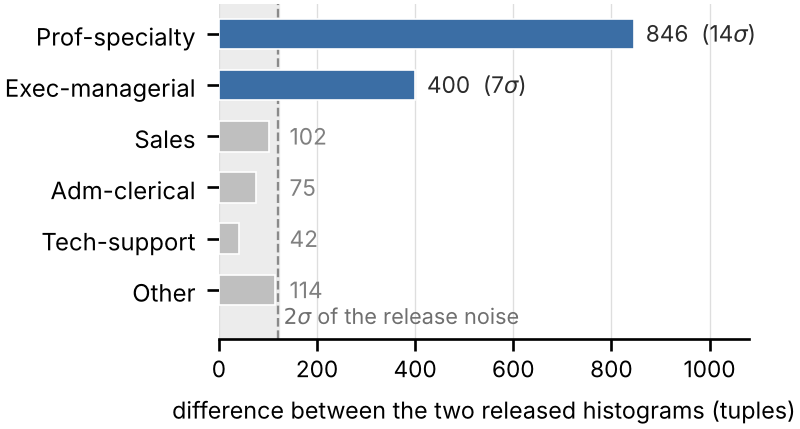
\includegraphics[width=\linewidth]{figures/released.png}
\caption{What the release leaves of the first explanation of the running example: the per-bin difference between the two noisy histograms of Figure~\ref{fig:candidates}(a). At $2k/\epsilon_H=30$ that difference has standard deviation $60$ per bin. Two bins clear twice it; the other four do not.}
\label{fig:released}
\end{figure}

\paragraph{The algorithms on the running example.}
Take the refinement of Example~\ref{ex:running} on Adult: $N=48{,}842$, $|\views|=1{,}052$, $|\Attrs|=10$, $k=5$, $\lambda=\tfrac12$ and $\epsilon=1$, so each stage receives $1/3$ and Eqs.~\eqref{eq:tau-rule} and~\eqref{eq:gamma-rule} give $\tau=15$ and $\gamma\approx150$.
Algorithm~\ref{alg:main} scores the $1{,}052$ views by $\Use$ and keeps $15$.
The view $\texttt{education}=\texttt{Masters}$ survives on a coverage of $0.068$ and a
representativeness of $0.80$, against the $0.92$ that Eq.~\eqref{eq:rep-upper} allows a view of
its size.
\added{At $\gamma_R=N$ it scored $0.53$, which is that ceiling exactly: the measure read none of
the reference attributes and would have returned $0.53$ whatever they held. The $0.12$ it now
falls short by is the distributional signal Eq.~\eqref{eq:gammaR-rule} leaves in.}

Algorithm~\ref{alg:topk} pairs it with each attribute, and the first round selects \texttt{occupation}, whose two histograms are those of Figure~\ref{fig:candidates}(a).
Figure~\ref{fig:released} shows what survives their release: the explanation is legible exactly where it is large, and the four small bins are returned as noise.
The counter of \texttt{occupation} is then incremented, and with $\lambda=\tfrac12$ every remaining candidate on that attribute is scored at half its value in the next round, which is what moves the second explanation onto a different attribute.

\paragraph{Exactness of the second stage.}
Because $\gamma$ is fixed once and the diversity factor depends only on attributes already released, the score of line~4 is the marginal gain of its candidate in the set objective of Definition~\ref{def:setobj}, so selecting the highest-scoring candidate is one step of greedy on it.
On that objective greedy is not an approximation but exact, because it separates over attribute groups and each group contributes a concave function of how many of its candidates are taken; Proposition~\ref{prop:greedy-exact} in Appendix~\ref{app:greedy} states both halves.
The optimality is over the candidates the view stage admits rather than over $\mathcal{E}$; what the filter discards is the cost Section~\ref{subsec:two-stages} leaves open.
This is what makes a non-private greedy run a usable reference point: with the candidate set and $\gamma$ held fixed it is the optimum, so the gap the private algorithm shows against it is attributable to the mechanism alone.

\subsection{Privacy and Cost}
\label{subsec:dp-proof}

\begin{proposition}[Sensitivity of the released histograms]
\label{prop:histogram-release-sensitivity}
Fix a candidate $(p,A)$ and write $H^j=\hist{Q_j(\pD)}{A}$ for $j=1,2$.
The pair $(H^1,H^2)$ has $L_1$-sensitivity at most $2$, and the difference $H^1-H^2$ has $L_1$-sensitivity at most $1$.
\end{proposition}

\begin{proof}
Since $Q_1$ and $Q_2$ are selections, one added tuple joins at most one bin of $A$, and it may be selected by both queries, by one of them, or by neither.
It therefore changes each of the two histograms in at most one coordinate and by at most $1$, which gives $2$ for the pair.
For the difference, the affected coordinate changes by $d_1-d_2$ with $d_1,d_2\in\{0,1\}$, so by at most $1$, and all other coordinates are unchanged.
\end{proof}

Releasing the pair therefore calls for $\Lap(2k/\epsilon_H)$, as in Algorithm~\ref{alg:topk}; the variant that releases only the difference uses $\Lap(k/\epsilon_H)$ for the same budget.

\begin{proposition}[Privacy of the framework]
\label{thm:alg1-dp}
Algorithm~\ref{alg:topk} satisfies $(\epsilon_S+\epsilon_H)$-differential privacy, and, with $N=|D|$ public as in Proposition~\ref{prop:usefulness-sensitivity}, Algorithm~\ref{alg:main} satisfies $\epsilon$-differential privacy.
\end{proposition}

\begin{proof}
Take Algorithm~\ref{alg:topk} first.
Each round invokes the exponential mechanism with budget $\epsilon_S/k$ on a utility of sensitivity $1/(1+\gamma)$ (Proposition~\ref{prop:selection-utility-sensitivity}), which is $(\epsilon_S/k)$-DP, and the Laplace mechanism with budget $\epsilon_H/k$ on a pair of histograms of $L_1$-sensitivity $2$ (Proposition~\ref{prop:histogram-release-sensitivity}), which is $(\epsilon_H/k)$-DP.
Both calibrations are legitimate because $\gamma$ is a constant of the mechanism rather than a function of the input: by Eq.~\eqref{eq:gamma-rule} it is determined by $k$, $|\views|$, $|\Attrs|$ and the budget, all of which are fixed before the data is read, so the sensitivity bound it induces holds uniformly over all databases.
The rounds are adaptive, since $u_i$ depends on the attributes already selected, but adaptive sequential composition applies~\cite{DBLP:series/synthesis/2016Li} and gives $k(\epsilon_S/k+\epsilon_H/k)=\epsilon_S+\epsilon_H$.
The conditioning covers the candidate set as well as the utility: $C_i$ is fixed by $\widehat{\mathcal{P}}$ and by what has already been released, both of them outputs of earlier steps, so for a fixed history it is the same set on neighbouring databases.

For Algorithm~\ref{alg:main}, view selection is $\epsilon_P$-DP by Theorem~\ref{thm:oneshot-topk} together with the sensitivity $\added{4/|D|}$ of Proposition~\ref{prop:usefulness-sensitivity}, which the algorithm passes to the mechanism.
This is the one place the hypothesis on $N$ is used, and it is used for the calibration rather than for the bound: Proposition~\ref{prop:usefulness-sensitivity} already covers neighbours of different sizes, but the theorem being invoked compares a \emph{single} mechanism on two inputs, and a $\Delta$ recomputed from each input would make the runs on $D$ and on $D'$ two different mechanisms.
\added{Fixing $\Delta=4/\bar N$ from a public $\bar N\le|D|$ that does not depend on $D$ removes that.}
Candidate construction is post-processing.
Sequential composition over the two stages gives $\epsilon_P+\epsilon_S+\epsilon_H=\epsilon$, so the pipeline as a whole is $\epsilon$-differentially private.
\end{proof}

\paragraph{Complexity.}
\label{subsec:complexity-analysis}
Let $|\mathcal{P}|$ be the number of candidate views, $a=|\Attrs|$ the number of explanation attributes, $r=|\mathcal{A}_R|$ the number of reference attributes, $b$ the maximum number of bins per attribute, and $N=|D|$.
Computing $\Use$ for every view costs $O(|\mathcal{P}|\,r\,N)$ by the direct route of one pass over $D$ per view, since $\Rep_{\gamma_R}$ averages over the reference attributes and every view needs its own histogram on each of them; the one-shot top-$\tau$ mechanism adds $O(|\mathcal{P}|\log\tau)$, one Gumbel draw per view and a heap of size $\tau$.
Materialising the bin vectors of the $\tau$ retained views over the $a$ explanation attributes costs $O(\tau a N)$.
Scoring is then paid once rather than once per round.
Because $\gamma$ is fixed by Eq.~\eqref{eq:gamma-rule}, $\HD_\gamma(p,A)$ is the same number in every round, so the $\tau a$ values are computed once in $O(\tau a b)$; a round only rescales each of them by its diversity factor, samples, and perturbs the two histograms of the winner, which is $O(\tau a+b)$.
The total is
\[
O\!\left(|\mathcal{P}|\,r\,N + \tau a\, N + \tau a b + k(\tau a + b)\right)
= O\!\left(\big(|\mathcal{P}|\,r + \tau a\big)N\right),
\]
because $b\le N$ and $k\le N$.
The two data passes therefore absorb everything else, and the $k$ selection rounds, the only part that spends privacy budget, cost $O(k(\tau a+b))$ and are independent of $N$.
Of the two passes only the first is independent of $k$ as well as of $\epsilon$; the second carries $\tau=\min(3k,|\mathcal{P}|)$.



\section{Experiments}
\label{sec:experiments}

This section evaluates the algorithm of Section~\ref{sec:solution} on real data.
All results below were produced on the real UCI Adult extract ($N=48{,}842$) and the real Tax benchmark ($N=500{,}000$).

\subsection{Experimental Goals}
\label{subsec:experimental-goals}

\begin{description}
  \item[RQ1 -- Use cases.] Do the released explanations identify the semantic change a refinement actually makes, on the query pairs the paper motivates?
  \item[RQ2 -- Scalability.] How does running time depend on $k$, $N$, $\epsilon$, $|\mathcal{P}|$, $\tau$, $\gamma$, and on the choice of algorithm?
  \item[RQ3 -- Quality.] How close is the private algorithm to non-private references, measured against three separate baselines?
\end{description}

\subsection{Experimental Setup}
\label{subsec:experimental-setup}

\subsubsection{Datasets and Query Pairs}
\label{subsubsec:datasets}

\paragraph{Adult.} The real UCI Adult extract, $48{,}842$ records.
We use two refinements, denoted Adult 6.7 (occupation broadening) and Adult 6.8 (education--hours), listed in Table~\ref{tab:query-pairs}.

\paragraph{Tax.} The real Tax benchmark used in the data-cleaning literature, $500{,}000$ records, with the marital-status refinement denoted Tax 6.6 in Table~\ref{tab:query-pairs}.

\paragraph{Not evaluated.}
IPUMS-CPS and the Stack Overflow Developer Survey are not included in this pass, and the Hospital/CQA setting is not evaluated at all: the framework has only ever been exercised on query-refinement pairs, never on a repair-semantics pair, and doing so would additionally require implementing repair semantics.
Section~\ref{sec:usecase-results} therefore substantiates the query-refinement use case only.

\begin{table}[t]
\centering
\small
\caption{Query pairs, on the real data. Each $Q$ violates its representation constraint and each $Q'$ satisfies it.}
\label{tab:query-pairs}
\begin{tabular}{@{}llrrr@{}}
\toprule
Pair & Constraint & $|Q|$ & $|Q'|$ & share in $Q\rightarrow Q'$ \\
\midrule
Adult 6.7  & $\ge25\%$ female   & 5{,}447  & 37{,}155  & $4.7\%\rightarrow26.9\%$ \\
Adult 6.8  & $\ge25\%$ female   & 3{,}055  & 2{,}453   & $19.5\%\rightarrow30.6\%$ \\
Tax 6.6    & $\ge30\%$ HasChild & 145{,}576 & 291{,}659 & $3.5\%\rightarrow50.1\%$ \\
\bottomrule
\end{tabular}
\end{table}

The Adult 6.8 figures reproduce the numbers quoted in Section~\ref{sec:introduction} ($19.5\%\rightarrow30.6\%$) exactly, on the real data.

\subsubsection{Parameters}
\label{subsubsec:parameters}

Unless stated otherwise $k=5$, $\lambda=0.5$, $\epsilon=1$, and the budget is split equally, $(\epsilon_P,\epsilon_S,\epsilon_H)=(\epsilon/3,\epsilon/3,\epsilon/3)$; $\tau$ and $\gamma$ follow Eqs.~\eqref{eq:tau-rule} and~\eqref{eq:gamma-rule}, giving $\tau=15$ and $\gamma\approx150$ on both datasets.
Equal shares is not an arbitrary default: sweeping the split over the three query pairs found no allocation that dominates it.
Equal shares gave the lowest released-histogram error on all three, and the best selection quality on the hardest of them.
Starving the view stage is the one clearly bad choice, since the explanation stage can only choose among the views that survive it: at $(0.10,0.55,0.35)$ the approximation ratio on Adult education-hours falls from $0.89$ to $0.57$.
Moving budget the other way buys a few points of selection quality on that pair alone and costs histogram accuracy on all three.
\alon{TODO: all numbers below were produced with $\tau=35$ and $\gamma=\lceil0.005N\rceil$ ($244$ for Adult, $2{,}500$ for Tax). They must be re-run under Eqs.~(\ref{eq:tau-rule}) and~(\ref{eq:gamma-rule}), \added{and now also under Eq.~(\ref{eq:gammaR-rule}), $\gamma_R=N/100$ in place of $\gamma_R=N$, with the view-stage sensitivity $\Delta=4/|D|$ of Proposition~\ref{prop:usefulness-sensitivity} in place of $7/(4|D|)$}. A first look on Adult education-hours, scored against a fixed yardstick so the comparison does not move with $\gamma$, put the new setting ahead of the old one, so the rerun is expected to improve rather than weaken the results.}
\alon{TODO (experiment to add): measure the view stage in isolation. For each query pair and each $\epsilon_P$, report the overlap between the privately retained $\tau$ views and the exact top-$\tau$ by $\Use$, and the lowest $\Use$ actually retained against the true $\tau$-th best. A first look at Adult education-hours suggests the overlap is low at the budgets used here and rises sharply with $\epsilon_P$, which would explain why the view stage is the one that must not be starved (Section~\ref{subsubsec:parameters}) and would give Section~\ref{subsec:two-stages} the empirical counterpart to the utility guarantee it lacks.}

Reported quantities average $40$ trials; this count is not incidental, as the between-trial standard deviation of set score is frequently comparable to its mean, and smaller counts cannot separate configurations reliably.

\subsection{Compared Methods}
\label{subsec:compared-methods}

We compare the algorithm of Section~\ref{sec:solution} against three baselines.

\begin{description}
  \item[B1 --- $\epsilon\rightarrow\infty$.] The identical algorithm, run with a privacy budget large enough that every mechanism is numerically deterministic. Isolates the cost of privacy noise alone, holding the architecture fixed.
  \item[B2 --- exhaustive optimum, non-private.] Enumerates \emph{all} size-$k$ subsets of the candidate explanations, scores each with the set-level objective of Definition~\ref{def:setobj}, and returns the maximiser.
  \item[B3 --- greedy, non-private.] Takes the top-$\tau$ views by $Usefulness$ with no privacy mechanism, then performs $k$ rounds selecting the best remaining histogram with no privacy mechanism.
\end{description}

B2 is exponential in $k$: with $\tau=35$ views and $10$ attributes the candidate space holds $350$ explanations and $\binom{350}{5}\approx5\times10^{11}$ subsets, which is not enumerable.
It is nevertheless computed \emph{exactly}, by restricting the search to the union over attributes of the top-$k$ candidates of each attribute group.
That restriction is lossless: if an optimal set contained a candidate outside the top-$k$ of its own group, some higher-scoring member of that group would be unused, and swapping it in cannot decrease $F_\lambda$, which is non-decreasing in the score of every member.
The pool is therefore $k\,|Attrs|=50$ candidates and $\binom{50}{5}\approx2.1\times10^{6}$ subsets, and B2 is the true optimum of the $\tau$-filtered space rather than an approximation to it.

\paragraph{Scoring.}
All four methods are scored on their output \emph{set} under one common yardstick: the paper's own objective, Definition~\ref{def:hd} with $\gamma_{\text{eval}}=0$, combined with the set-level utility of Definition~\ref{def:setobj}.
This is deliberate. Smoothing is a mechanism-internal device, and allowing it to define the metric as well would make the comparison circular; scoring at $\gamma_{\text{eval}}=0$ means the algorithm is judged by the standard of the unmodified paper even though it selects under smoothing.

\subsection{Use Case Results}
\label{sec:usecase-results}

\begin{figure}[t]
\centering
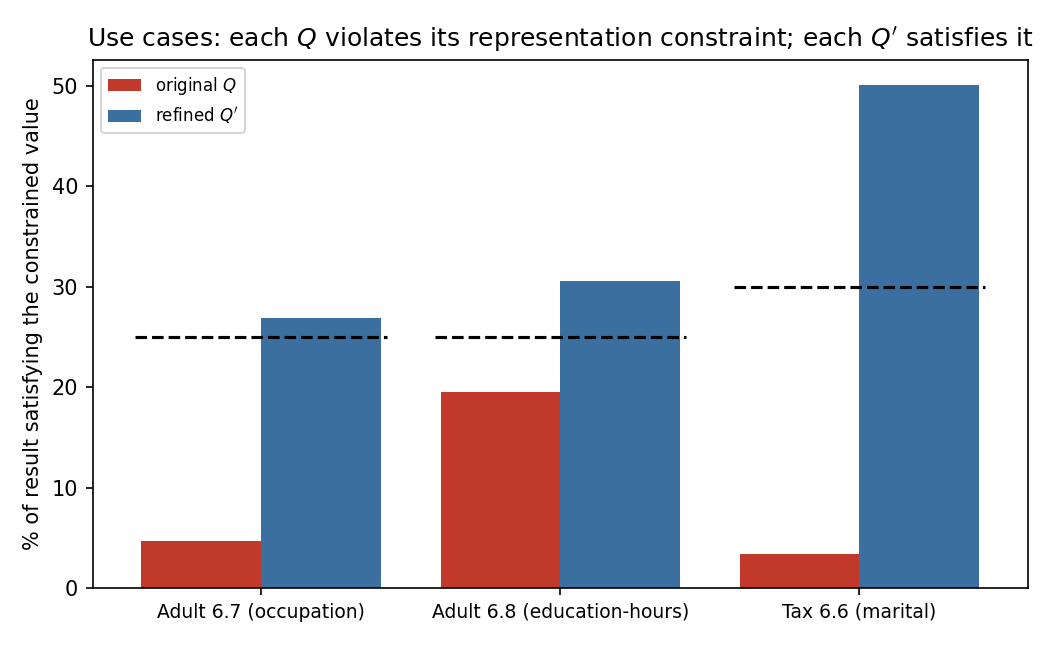
\includegraphics[width=\linewidth]{figures/U1_constraint_premise.png}
\caption{Each original query violates its representation constraint (dashed line) and each refined query satisfies it, on the real data.}
\label{fig:premise}
\end{figure}

Figure~\ref{fig:premise} establishes the premise: on real data all three refinements do what the motivating examples claim.
Figures~\ref{fig:rel-tax}--\ref{fig:rel-adult-edu} show the differentially private explanations the algorithm releases for each pair at $\epsilon=1$, $k=5$.

\begin{figure}[t]
\centering
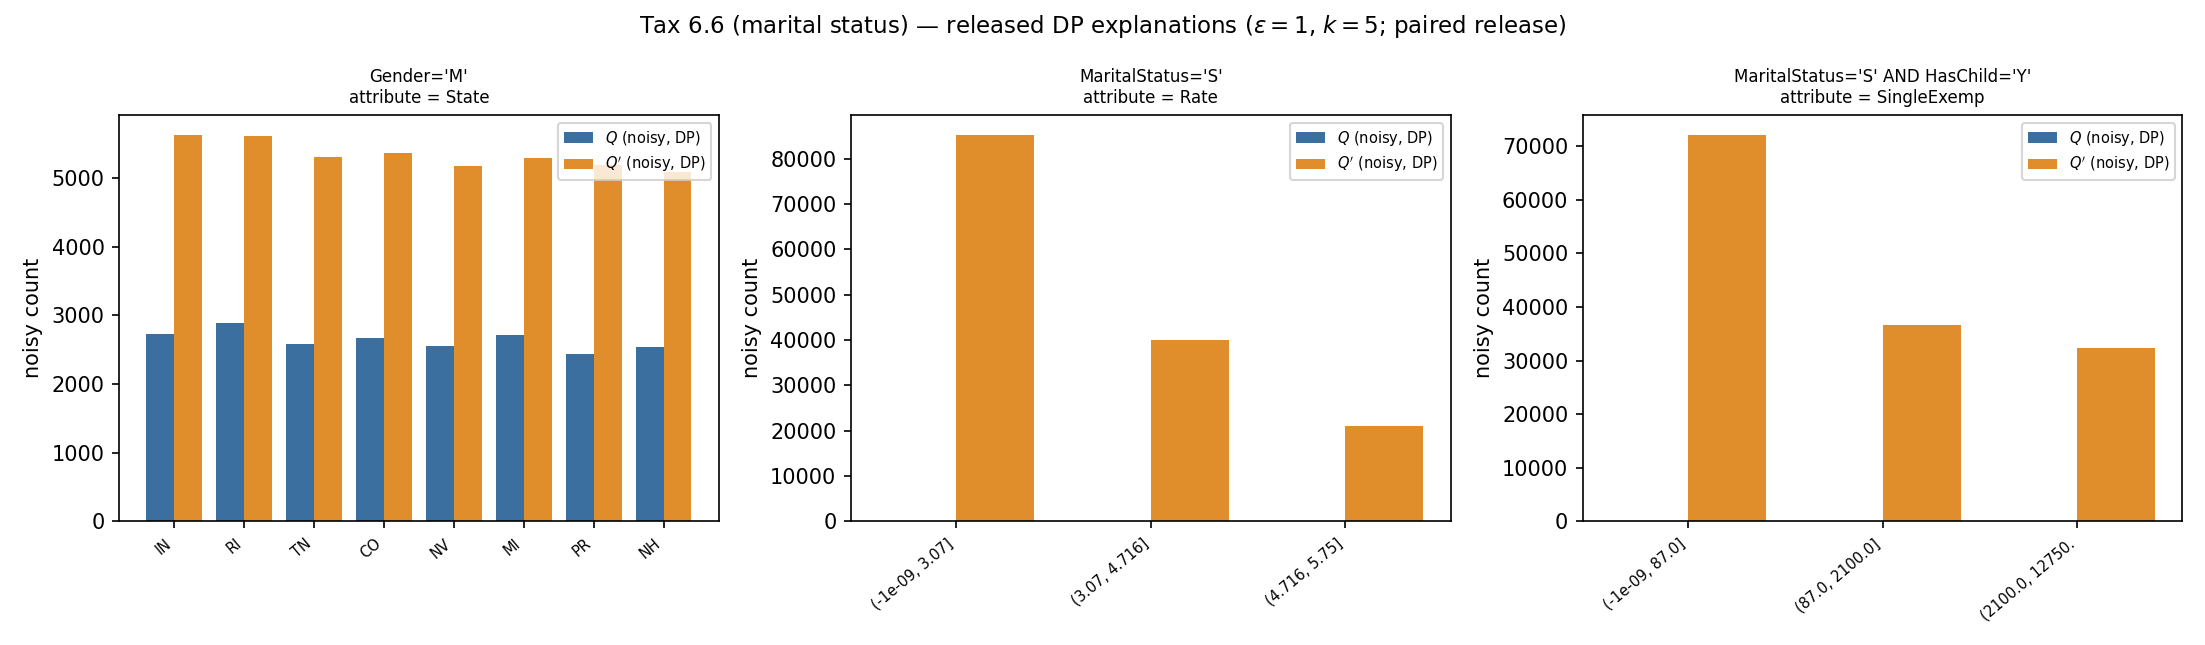
\includegraphics[width=\linewidth]{figures/U2_released_tax_marital.png}
\caption{Tax 6.6 --- released differentially private explanations.}
\label{fig:rel-tax}
\end{figure}

For Tax the refinement removes the predicate $\texttt{MaritalStatus}=\texttt{'M'}$.
The algorithm recovers exactly that subgroup: three of the five released explanations are conditioned on $\texttt{MaritalStatus}=\texttt{'S'}$, the population the refinement mechanically introduces, with a shift of $-85{,}178$ tuples concentrated in the lowest \texttt{Rate} bucket.
The framework is never given the query predicates.

\begin{figure}[t]
\centering
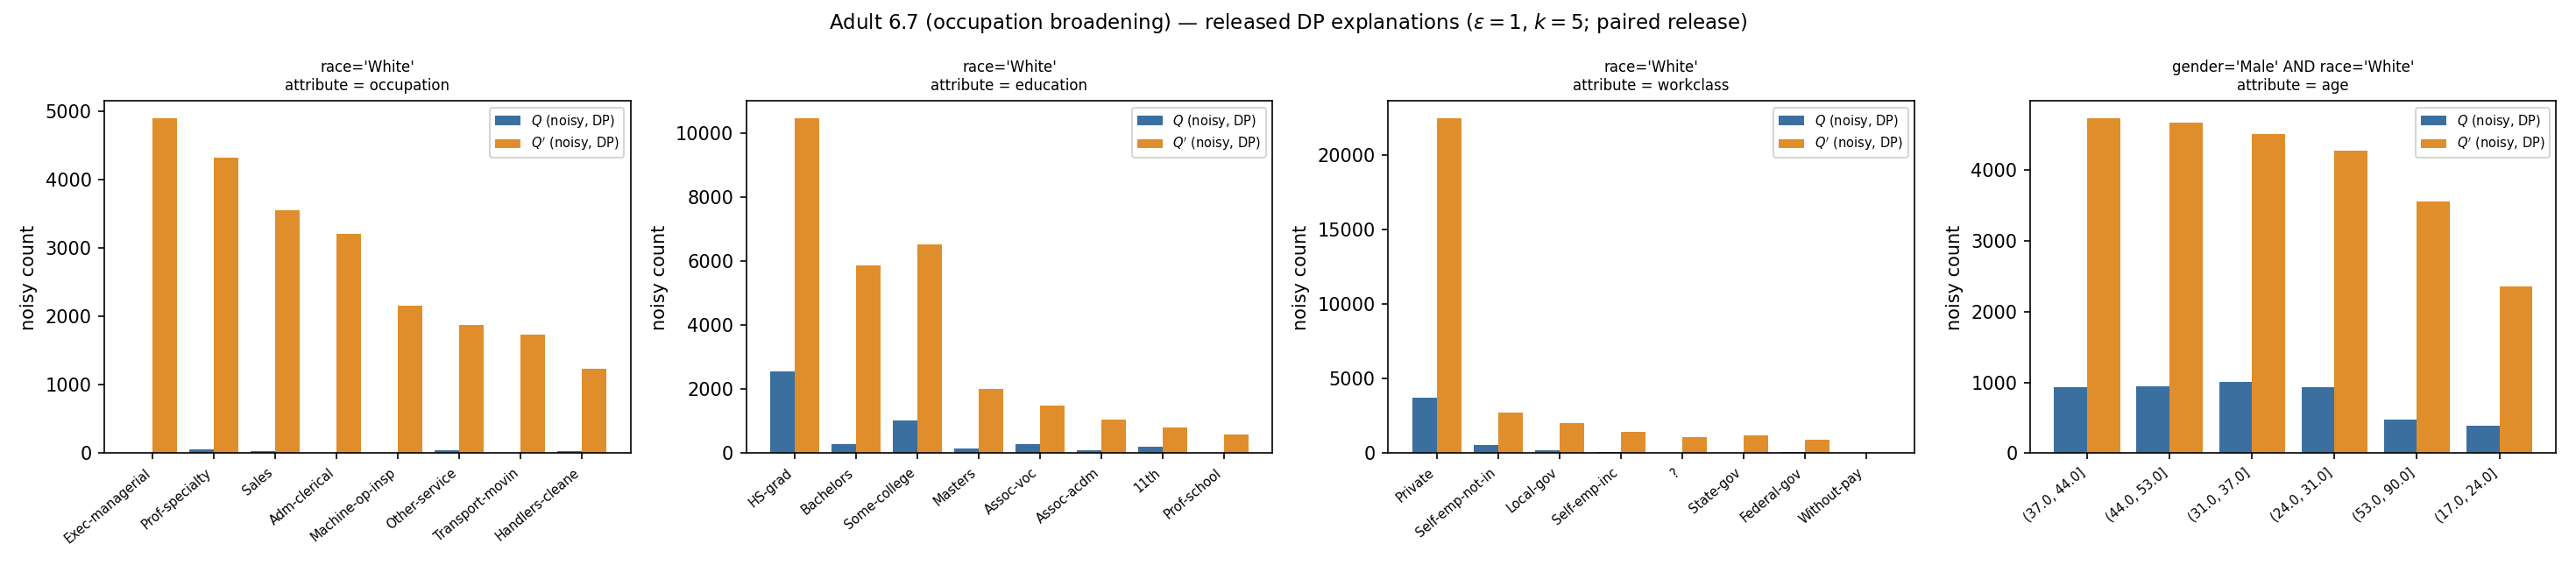
\includegraphics[width=\linewidth]{figures/U2_released_adult_occupation.png}
\caption{Adult 6.7 --- released differentially private explanations.}
\label{fig:rel-adult-occ}
\end{figure}

\begin{figure}[t]
\centering
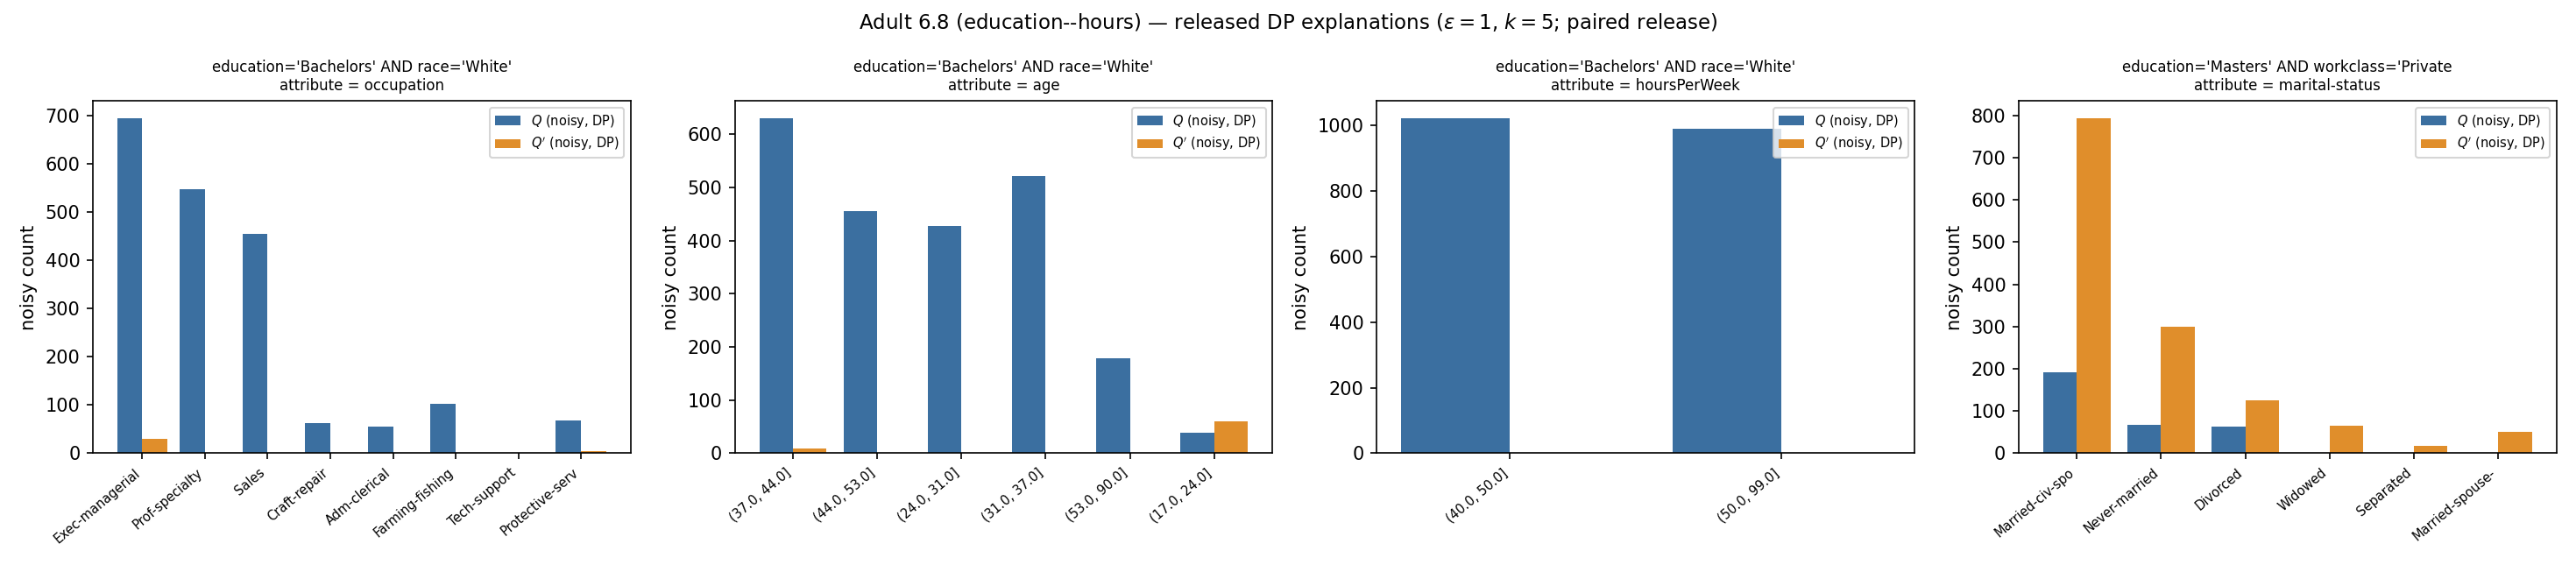
\includegraphics[width=\linewidth]{figures/U2_released_adult_education_hours.png}
\caption{Adult 6.8 --- released differentially private explanations.}
\label{fig:rel-adult-edu}
\end{figure}

For Adult 6.7 the released explanations are dominated by shifts \emph{within} $\texttt{race}=\texttt{'White'}$ across \texttt{occupation}, \texttt{education} and \texttt{workclass}, showing that broadening a narrow occupational query changes the occupational and educational composition of the result rather than merely enlarging it.
For Adult 6.8 the explanations localise on $\texttt{education}=\texttt{'Bachelors'}$ subgroups, which is the population the refinement removes when it restricts education to \texttt{Masters}.

These are the un-cherry-picked outputs of a single run at the default parameters.

\subsection{Scalability}
\label{subsec:scalability}

\begin{figure*}[t]
\centering
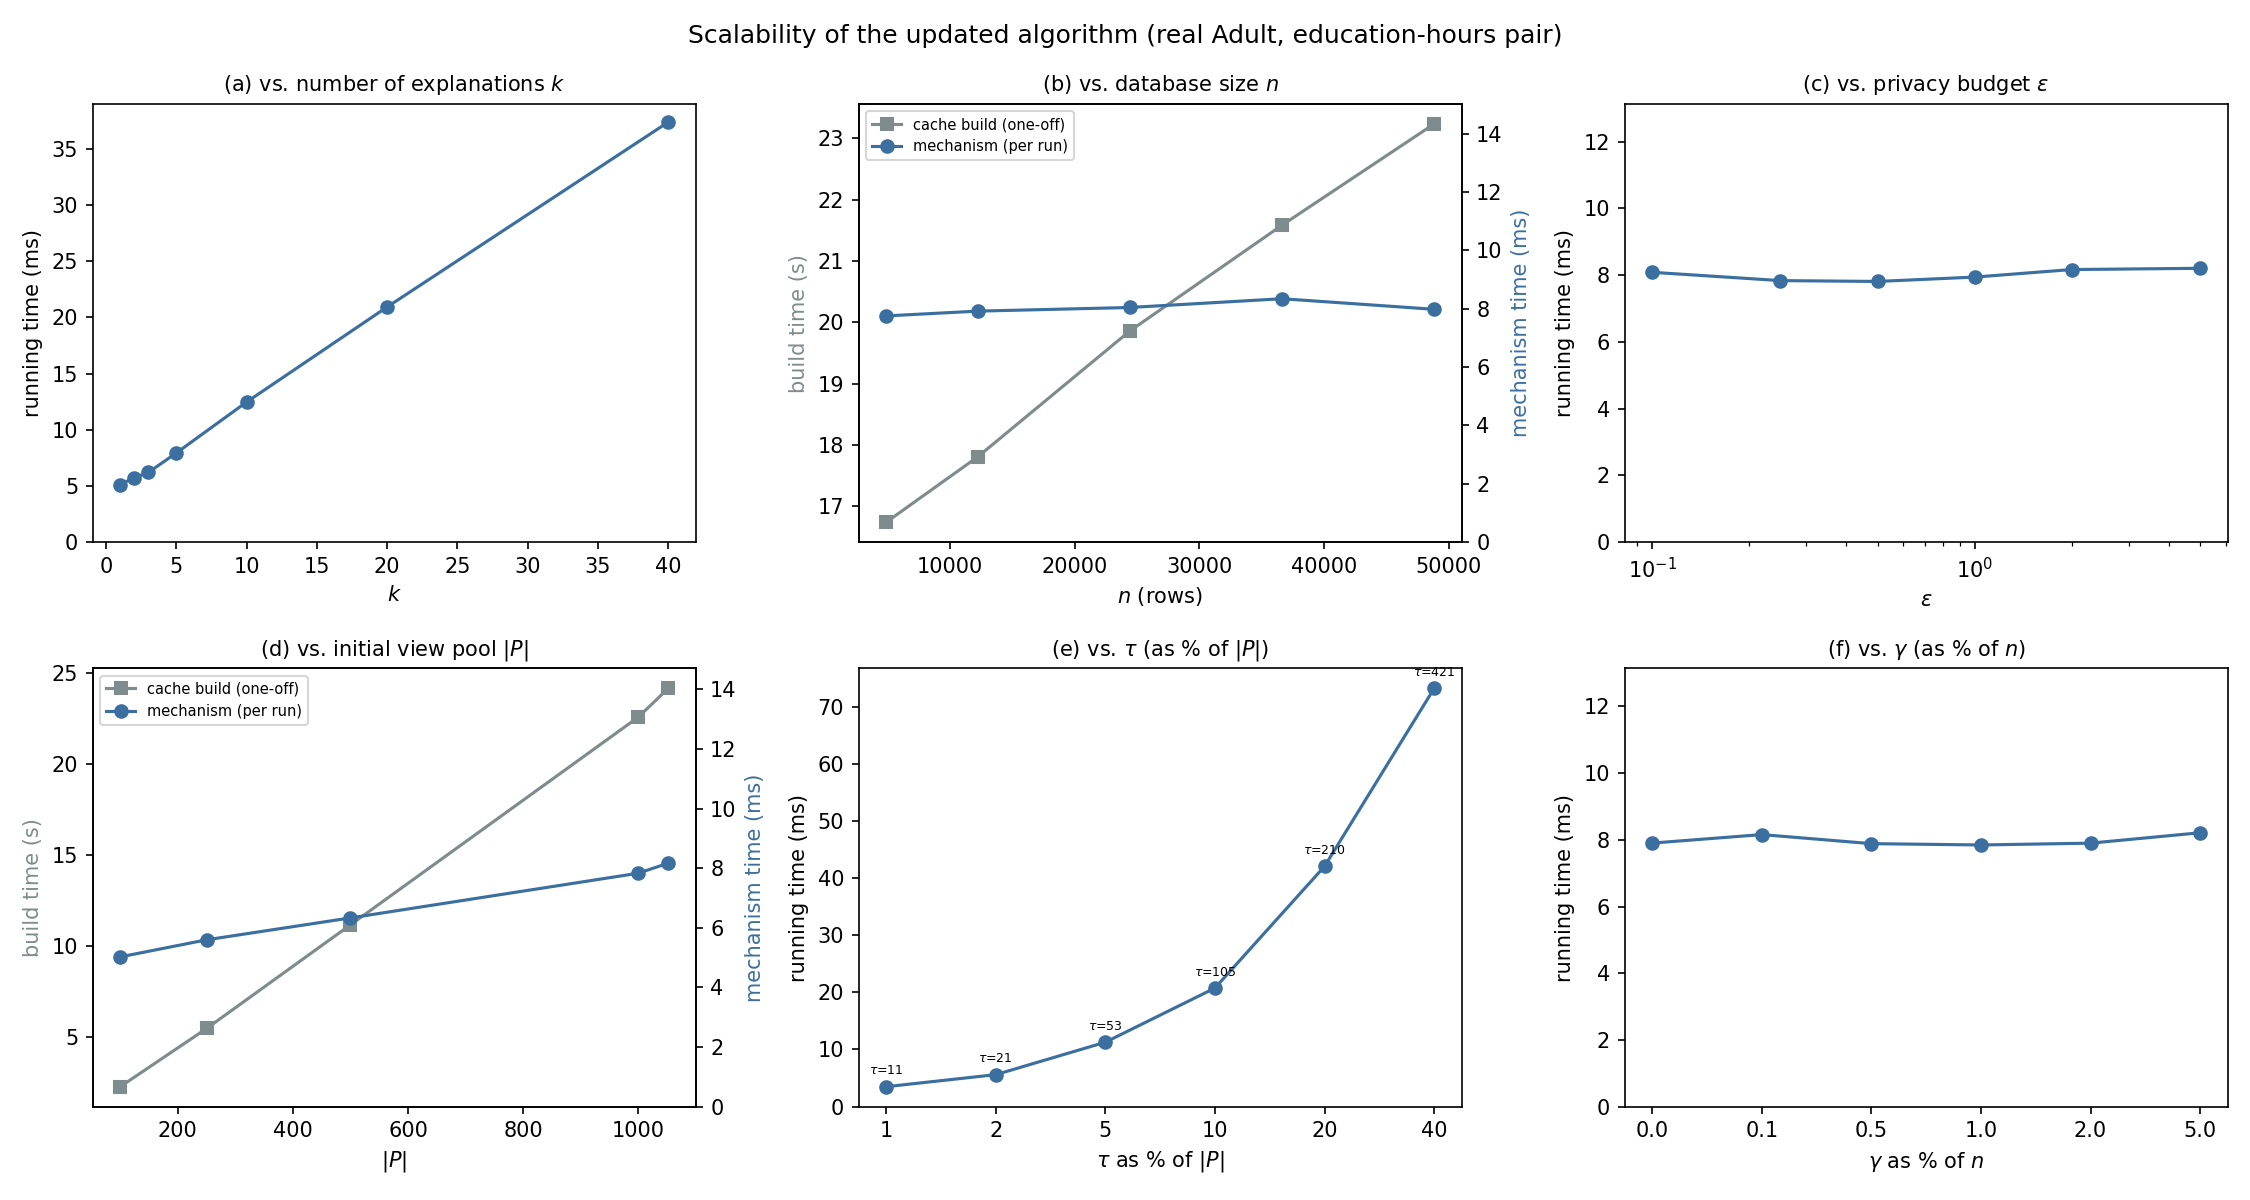
\includegraphics[width=\linewidth]{figures/S1_scalability_grid.png}
\caption{Running time of the algorithm. Panels (b) and (d) separate the one-off cache build, which carries the $O(N)$ and $O(|\mathcal{P}|)$ work, from the per-invocation mechanism cost.}
\label{fig:scalability}
\end{figure*}

Figure~\ref{fig:scalability} reports the six sweeps.

\paragraph{$k$, $\tau$, $|\mathcal{P}|$.}
Running time is linear in $k$ ($4.6$\,ms at $k=1$ to $36.3$\,ms at $k=40$) and in $\tau$, matching the $O(k\tau m b)$ term of Section~\ref{subsec:complexity-analysis}.
Expressed as a fraction of $|\mathcal{P}|$, moving $\tau$ from $5\%$ to $10\%$ doubles per-round cost ($11.1$\,ms to $19.9$\,ms) and from $5\%$ to $40\%$ multiplies it sevenfold.

\paragraph{$N$ and $|\mathcal{P}|$.}
The per-invocation cost is essentially flat in $N$ ($7.7$--$8.3$\,ms across a tenfold range), because the $O(N)$ work is confined to the one-off preprocessing, which grows from $16.7$\,s to $23.2$\,s over the same range.
Panels (b) and (d) plot both; presenting only the per-run curve on an autoscaled axis would turn a sub-millisecond spread into an apparent trend.

\paragraph{$\epsilon$ and $\gamma$.}
Running time is invariant to both ($7.8$--$8.2$\,ms across $\epsilon\in[0.1,5]$, and $7.9$--$8.3$\,ms across $\gamma$ from $0\%$ to $5\%$ of $N$).
For $\epsilon$ this is the expected result and confirms no budget-dependent overhead.
For $\gamma$ it is a consequence of the caching described in Section~\ref{subsec:complexity-analysis}: $\gamma$ enters only the denominator, so changing it costs nothing.
This is what makes re-scoring at a different $\gamma$ free in running time as well as in privacy.

\subsubsection{Running Time by Algorithm}
\label{subsec:runtime-algorithm}

\begin{figure}[t]
\centering
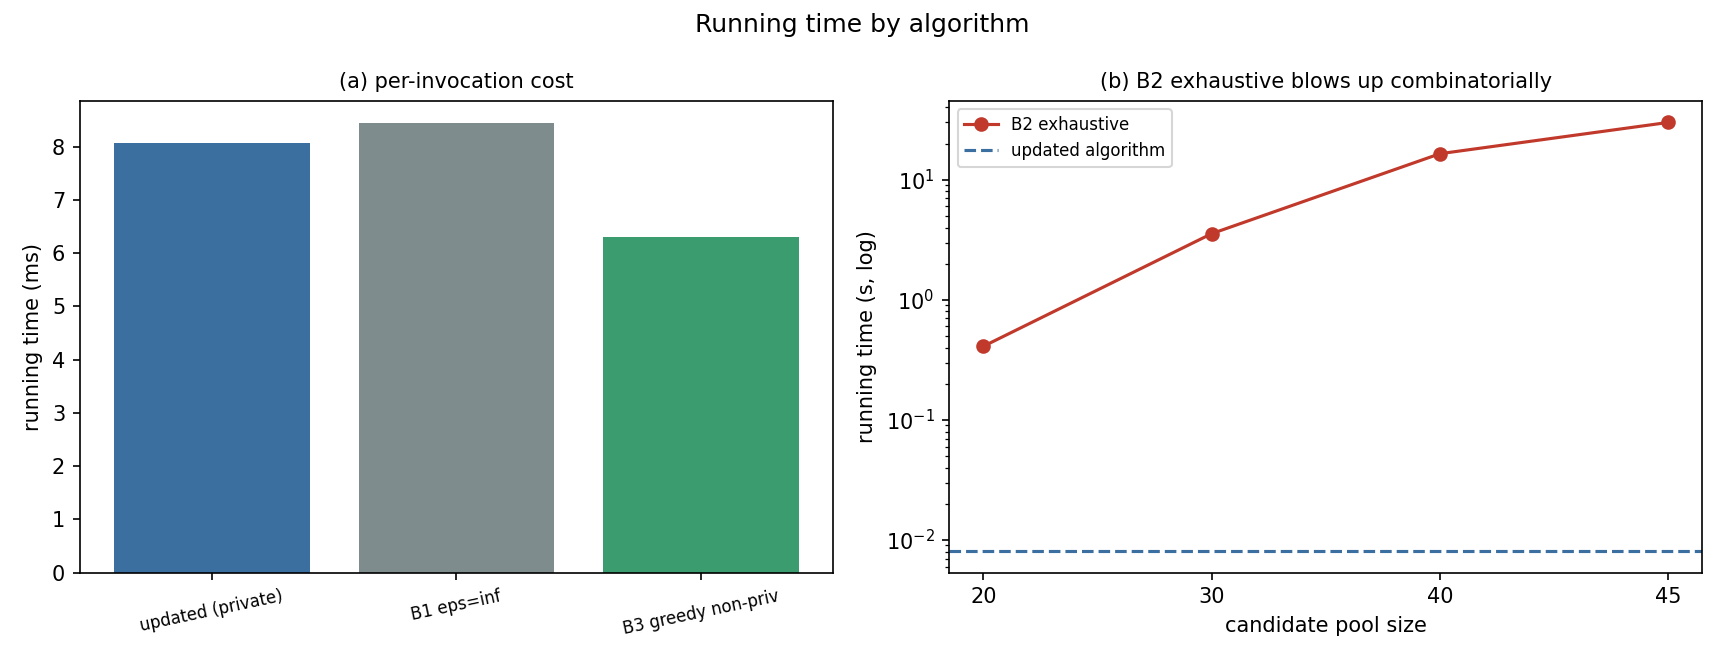
\includegraphics[width=\linewidth]{figures/S2_runtime_by_algorithm.png}
\caption{Per-invocation cost of each method, and the combinatorial blow-up of the exhaustive baseline B2.}
\label{fig:runtime-algorithm}
\end{figure}

The private algorithm ($8.1$\,ms), B1 ($8.4$\,ms) and B3 ($6.3$\,ms) are all within a small constant of one another: privacy costs essentially nothing in running time, since the exponential mechanism replaces an $\arg\max$ over the same scores.

B2 is different in kind.
On a $20$-candidate pool it takes $0.41$\,s; at $30$, $3.6$\,s; at $40$, $16.5$\,s; at $45$, $30.0$\,s --- a $73\times$ increase for a $2.25\times$ increase in pool size, tracking $\binom{|C|}{5}$.
On the lossless $50$-candidate pool it takes $57$\,s, versus $8$\,ms for the private algorithm.
Enumerating the unrestricted $350$-candidate space would take on the order of months, which is why the losslessness argument above is needed rather than optional, and why the selection is run greedily: by Proposition~\ref{prop:greedy-exact} that costs nothing in quality.

\subsection{Quality}
\label{subsec:quality}

\begin{figure*}[t]
\centering
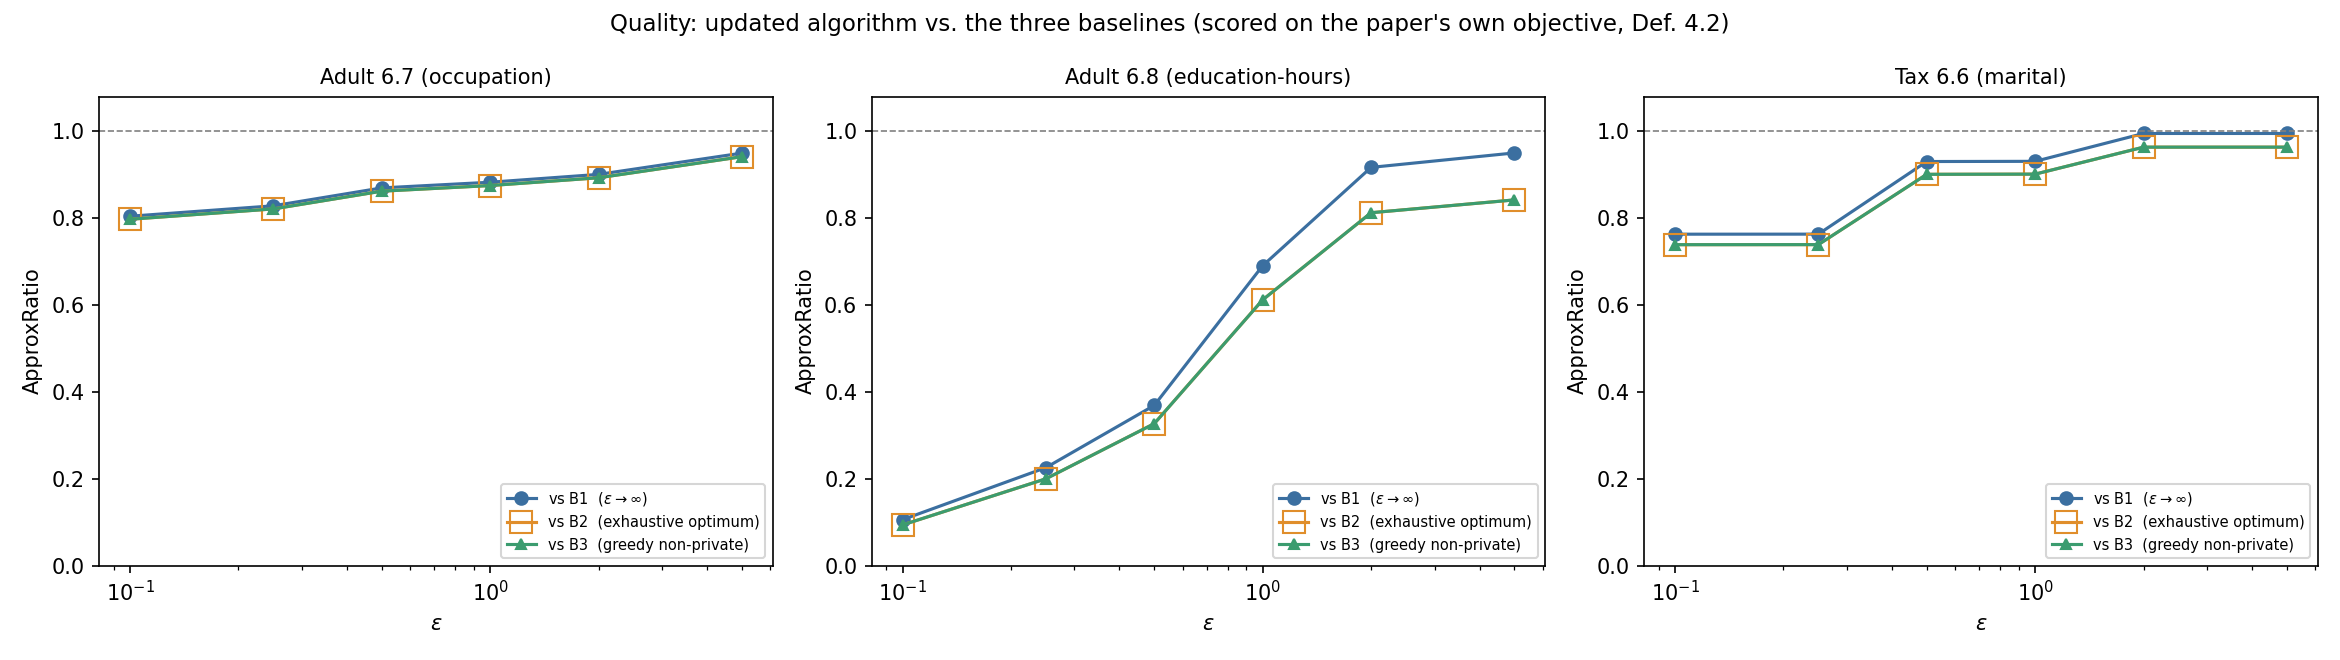
\includegraphics[width=\linewidth]{figures/Q1_approxratio_vs_baselines.png}
\caption{ApproxRatio of the algorithm against each baseline, scored on the paper's own objective ($\gamma_{\text{eval}}=0$), $40$ trials per point.}
\label{fig:quality}
\end{figure*}

\begin{table}[t]
\centering
\small
\caption{ApproxRatio against each baseline at $\epsilon=1$ and $\epsilon=5$.}
\label{tab:quality}
\begin{tabular}{@{}lcccccc@{}}
\toprule
& \multicolumn{3}{c}{$\epsilon=1$} & \multicolumn{3}{c}{$\epsilon=5$}\\
\cmidrule(lr){2-4}\cmidrule(lr){5-7}
Pair & B1 & B2 & B3 & B1 & B2 & B3\\
\midrule
Adult 6.7 & 0.883 & 0.875 & 0.875 & 0.950 & 0.941 & 0.941\\
Adult 6.8 & 0.691 & 0.612 & 0.612 & 0.950 & 0.842 & 0.842\\
Tax 6.6   & 0.931 & 0.901 & 0.901 & 0.995 & 0.963 & 0.963\\
\bottomrule
\end{tabular}
\end{table}

At the default $\epsilon=1$ the algorithm attains $0.88$--$0.93$ of the $\epsilon\rightarrow\infty$ reference on two of the three pairs and $0.88$--$0.90$ of the exhaustive optimum, rising to $0.94$--$1.00$ and $0.94$--$0.96$ respectively at $\epsilon=5$.
Adult 6.8 is the hardest pair and the only one that degrades sharply at small $\epsilon$ ($0.11$ against B1 at $\epsilon=0.1$); it is also the pair whose top candidates are most tightly bunched, so the exponential mechanism has the least separation to exploit.

Two observations are worth isolating.

First, \textbf{B2 and B3 coincide exactly on all three query pairs} (Figure~\ref{fig:absolute}): the non-private greedy procedure attains the true optimum of the $\tau$-filtered space, not merely an approximation to it.
This is what Proposition~\ref{prop:greedy-exact} predicts: on a fixed candidate set and a fixed $\gamma$ greedy returns the exact maximiser, so the two references answer the same question here.
The measurement confirms it on real instances rather than establishing it.

Second, the ratio against B2/B3 is consistently slightly below the ratio against B1.
B1 holds the architecture fixed and removes only the noise, so it isolates the cost of privacy; B2/B3 remove the noise \emph{and} search without a privacy-imposed $\tau$ budget, so the residual gap to them also includes what the mechanism gives up by having to select views privately at all.
Reporting both separates those two costs.

\begin{figure}[t]
\centering
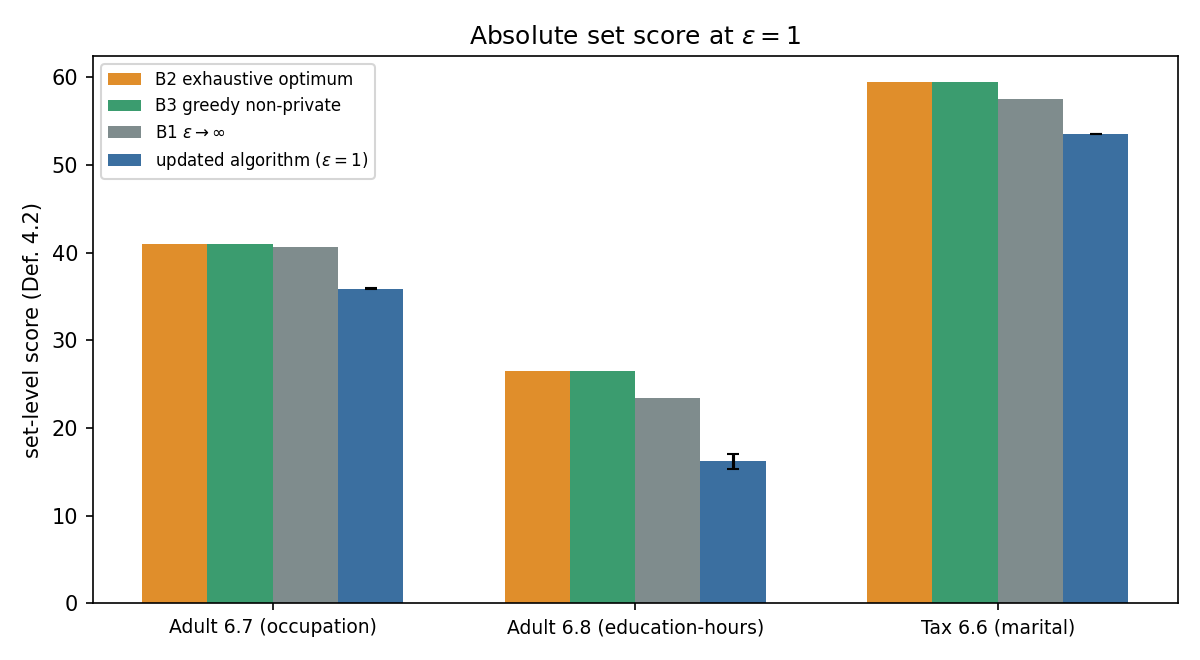
\includegraphics[width=\linewidth]{figures/Q2_absolute_scores.png}
\caption{Absolute set scores at $\epsilon=1$. B2 and B3 coincide exactly: non-private greedy attains the exhaustive optimum on every pair.}
\label{fig:absolute}
\end{figure}

\subsubsection{The $\gamma$ Trade-off}
\label{subsec:gamma-tradeoff}

Smoothing is not free, and the cost is worth stating precisely.
$\gamma$ competes against the size of individual histogram \emph{bins}, and the bin-count distribution relative to $|D|$ differs sharply between datasets: the median non-empty bin holds $20$ tuples on Adult but $3{,}897$ on Tax, a factor of $200$ despite only a factor of $10$ in $N$.
Consequently the same "fraction of $N$" rule lands in very different regimes.
At $\gamma=0.5\%$ of $N$, $\gamma$ exceeds the bin count for $84\%$ of Adult bins but only $30\%$ of Tax bins; at $5\%$ of $N$ it exceeds $98\%$ and $94\%$ respectively, at which point the median ratio $m_v/(m_v+\gamma)$ falls to $0.008$ on Adult and $HD_\gamma$ has effectively stopped measuring \emph{relative} change at all.

The pre-registered rule of Section~\ref{subsubsec:parameters} is therefore defensible but crude, and $\gamma$ at $5\%$ of $N$ would be clearly too aggressive.
A sharper anchor follows from Proposition~\ref{prop:hd-sensitivity}: the separation available to the exponential mechanism scales as $\epsilon\,\delta u\,(1+\gamma)/2$, so the $\gamma$ actually required is governed by the \emph{margin} between the leading candidates rather than by $N$.
Measured on the three pairs, that margin is $0.027$, $0.121$ and $0.315$ respectively, implying required $\gamma$ of roughly $292$, $66$ and $25$ --- an ordering unrelated to dataset size, and inverted with respect to it.

\subsection{Summary of Findings}
\label{subsec:experiments-summary}

Running time is linear in $k$, $\tau$ and $|\mathcal{P}|$, invariant to $\epsilon$ and $\gamma$, and independent of $N$ once preprocessing is amortised; privacy adds no measurable cost relative to the non-private greedy baseline, while the exhaustive baseline is intractable beyond a few dozen candidates.
On quality the algorithm reaches $0.88$--$0.93$ of the $\epsilon\rightarrow\infty$ reference at the default budget and $0.95$--$1.00$ at $\epsilon=5$, judged by the paper's own unsmoothed objective; non-private greedy attains the exhaustive optimum exactly on all three pairs, as Proposition~\ref{prop:greedy-exact} predicts.
The use cases show that the released explanations localise the population a refinement adds or removes without being given the query predicates --- most sharply on Tax, where three of five released explanations recover exactly the subgroup the dropped predicate introduces.
The principal caveat is the choice of $\gamma$: it is what makes private selection work at these budgets, but anchoring it to a fraction of $|D|$ is a crude proxy for the quantity that actually determines it.

\section{Related Work}
\label{sec:related}

We discuss three lines of work: how the pair of query outputs that we explain is produced, how existing systems explain query results and differences between data, and how differential privacy has been used for explanations. To our knowledge, no prior work generates differentially private explanations for the differences between two related query outputs.

\emph{Query refinement and repair.}
Query refinement has been studied for queries with empty answers~\cite{muslea2005online,KoudasLTV06} and for queries that must meet constraints on the size of the output~\cite{MK09,chu1994structured}.
Recent work refines queries to satisfy diversity and representation constraints.
Erica~\cite{ERICA,LMSJ23} changes a query so that the result meets constraints on the sizes of several subgroups. It uses provenance annotations to do this efficiently.
The work in~\cite{SSAD22} finds a fair query that is close to the user's query. It supports range predicates and a binary sensitive attribute.
The work in~\cite{CSSM24} changes the selection conditions of top-$k$ queries.
Provenance has also been used to analyze and reduce bias in data-driven tools~\cite{MLJ22}.
In consistent query answering, queries are evaluated over the repairs of an inconsistent database~\cite{arenas1999,bertossi2006,bertossi2011}.
These systems return a refined query or a repaired answer. They give limited support for explaining what the change means for the data.
Our framework treats the process that produces the second output as a black box, so it can be used together with these systems (Section~\ref{subsec:prelim-settings}).

\emph{Explaining query results and data.}
Provenance~\cite{buneman2001,cheney2009,herschel2017} tracks why and where output data comes from.
Intervention-based work~\cite{RoyS14} explains an aggregate result with predicates that select tuples whose removal changes the result.
Scorpion~\cite{wu2013} finds predicates that explain outliers in aggregate results using properties of the input tuples.
Why-not questions~\cite{CJ09,tran2010conquer} ask why some tuples are missing from a query result.
CAPE~\cite{MZGR19} explains an outlier in an aggregate result by values that deviate in the opposite direction.
MacroBase~\cite{MacroBase} explains outliers with attribute-value combinations that are common among outliers and rare among inliers. It ranks them with the relative risk ratio.
DIFF~\cite{DIFF} is a relational operator that provides the functionality of such explanation engines.
Some works are closer to ours.
SeeDB~\cite{SeeDB} scores a view by the distance between its distributions on a target subset and on a reference subset.
FEDEX~\cite{FEDEX} scores a data exploration step by how much it changes the distribution of an attribute.
Contrast set mining~\cite{BayPazzani01} and emerging patterns~\cite{DongLi99} look for conjunctions of attribute values whose distribution or support differs between groups or datasets.
We use the interestingness, coverage, representativeness and diversity measures from this literature (Section~\ref{subsec:prelim-quality}).
However, these works mainly explain a single query result, a prediction, or a data transformation. They do not explain the differences between two related query outputs.
In addition, explanations based on individual tuples cannot be used under differential privacy~\cite{TaoGMR22}.

\emph{Differential privacy for explanations.}
DPXPlain~\cite{TaoGMR22} explains aggregate query results under differential privacy.
The user compares the aggregate values of two groups in a query result.
DPXPlain releases noisy answers, a confidence interval for the difference between the groups, and a table of top-$k$ explanation predicates.
The predicates are selected with the one-shot top-$k$ mechanism~\cite{DurfeeRogers19}.
DPClustX~\cite{DPClustX} explains clustering results under differential privacy using histograms. It works in two stages.
It replaces quality measures with high sensitivity by measures with low sensitivity.
Like both works, we use private selection. Like DPClustX, we release noisy histograms and use quality measures with low sensitivity.
Our setting is different. We explain the difference between two related query outputs, such as a query and its refinement.
Our quality measures are defined for this comparison (Section~\ref{sec:explanation-quality}).
Each explanation is a pair of noisy histograms of an attribute inside a selected view.
Systems for differentially private data analysis~\cite{mcsherry2009,JNS18,JNHS20} support aggregate queries. As noted in~\cite{TaoGMR22}, private SQL systems do not support explanations.
We build our algorithms from known mechanisms: the exponential mechanism~\cite{mcsherry2007}, one-shot top-$k$~\cite{DurfeeRogers19} and the Laplace mechanism~\cite{DMNS2006}.
We smooth the denominators of ratio-based scores to bound their sensitivity. A similar idea is used in differentially private decision trees~\cite{FriedmanSchuster10} and in~\cite{DPClustX}.


% Deprecated section
% \input{sections/provenance}

% \section{Finding The Best Approximation}
\label{sec:search}

Our problem may be solved na\"{\i}vely by an exhaustive search over the possible refinements. However, the search space of refinements becomes intractably large even with relatively modest datasets, as the number of possible refinements is exponential in the number of the query's attributes.
% the sum of $\domain(\pi_A(D))$ for every categorical attribute $A$ with a predicate over it.
%\felix{was shown in \cite{LMSJ23} where the number of possible refinements is bounded by $$\mathcal{O} \left( \Pi_{(A \diamond C) \in \num(Q)} |\domain(\pi_A(D))| \cdot 2^{\sum_{(\bigvee_{c \in C} A = c) \in \cat(Q)} \domain(\pi_A(D)} \right)$$}. 
Beyond the high cost of an exhaustive search, a na\"{\i}ve solution would require the evaluation of each refinement query on the DBMS to check its deviation from the constraint set. 

To address these challenges, we propose a solution based on a mixed-integer linear program (MILP). Mixed-integer linear programming is a model for optimizing a linear objective function subject to a set of expressions (equalities and inequalities) linear in the discrete or continuous variables of the problem, limiting the space of feasible assignments. Solvers for such programs have been developed with techniques to solve even large problems efficiently in practice, as discussed in \cite{QFix}.
%\yuval{is tractable a correct term here? I believe the problems are still hard but can be solved efficiently in practice}
By incorporating the concepts introduced in~\cite{MLJ22, ERICA}, we utilize data annotations to depict potential refinements. These annotations serve as variables in the MILP, and enable us to quantify the deviation from the constraint set without having to reevaluate refinements across the DBMS.

Briefly, a solution for a MILP is an assignment for the variables in the expressions, such that they are satisfied and the objective function is minimized. 
Intuitively, given a database $D$, a query $Q$, a constraint set $\constraints$, a maximum deviation from the constraint set $0 \leq \varepsilon$, and a distance measure $DIS$, we construct an instance of MILP such that the solution corresponds to a minimal refinement that produces a ranking such that its deviation is within the maximum deviation $\varepsilon$ from the constraint set $\constraints$ while minimizing $DIS$.
By formulating \problem{} as a MILP, we can leverage existing tools to streamline the search process. 


It is important to note that by using MILP to represent the problem, we are limited to distance measures that can be modeled by a linear program. However, this limitation still allows a wide range of useful distance measures, including the ones defined in~\Cref{sec:distance}. Some of these measures may require additional modeling techniques to become linearized. For example, when modeling the Jaccard distance, we can use the Charnes-Cooper transformation~\cite{CC62}. Similarly, we can introduce auxiliary binary variables to model the version of Kendall's $\tau$ for top-$k$ lists introduced in \cite{FKS03}. %\julia{Maybe this is a better place to say what you do for Fagin's version of Kendall's tau.} \felix{$\leftarrow$ check 15/10}

\begin{table}[t!]
    \centering
    \caption{Summary of variables used in our MILP model}
    %\vspace{-0.5cm}
    \footnotesize
    \begin{tabularx}{0.48\textwidth}{c|c|X}
    {\bf Var.} & \revc{{\bf Domain}} & {\bf Description} \\
    \hline
    %  $C_{A, v}$        & Whether $v$ is included in $C$ for a cat. predicate on $A$                              \\
    $C_{A,\diamond}$  & \revc{$\mathbb{R}$} & Refined $C$ for a num. predicate on $A$ with operator $\diamond$                     \\
    $A_v$             & \revc{$\{0, 1\}$} & Whether a value $v$ is selected by the cat. predicate on $A$                           \\
    $A_{v, \diamond}$ & \revc{$\{0, 1\}$} &  Whether a value $v$ is in the range of the num. predicate on $A$ with operator $\diamond$ \\
    $r_t$            & \revc{$\{0, 1\}$} & Whether tuple $t$ is selected by the refinement                                     \\
    $s_{t}$          & \revc{$\mathbb{R}$} & Rank of tuple $t$ in the ranking generated by the refinement                              \\
    $l_{t, k}$       & \revc{$\{0, 1\}$} & Whether tuple $t$ is present in the top-$k$ of the ranking generated by the refinement          \\
    $E_{G, k}$       & \revc{$\mathbb{R}$} & Number of tuples to add (remove) to satisfy lower-bound (upper-bound) cardinality constraint    
    \end{tabularx}
    % \vspace{-1cm}
    %\yuval{TODO: update}
    \label{tab:variables}
\end{table}

The MILP instance we construct consists of two main groups of expressions: those that require that all tuples selected by the refinement are in the ranking according to the {\tt ORDER BY} expression of $Q$, and those that enforce that the derived ranking's deviation from the constraint set does not exceed the input bound $\varepsilon$. We next explain the construction of the expressions in each set\revc{, and, in order to give a more intuitive picture of the process, demonstrate in \Cref{fig:example_summary} how variables are generated from a running example and how they are combined by these expressions.}


\subsection{Modeling refinements output using expressions}

Inspired by the use of provenance for query refinements~\cite{MLJ22,ERICA}, we utilize the notion of data annotations to model refinements through a set of expressions. This set is divided into two parts. The first part is used to model the tuples that satisfy the refinement query's predicate, while the second part ensures that the selected tuples are ordered correctly by the {\tt ORDER BY} expression of the input query. We start by describing the variables used in the expressions.



% \begin{table}[ht]
%         \centering
		
% 		\label{tab:joined}
%         \hspace*{-0.5cm}
%         \footnotesize
% 		\begin{tabular}{crccrrcc}
% 		\cline{2-8}
% 		& \textbf{ID} & \textbf{Gender} & \textbf{Income} & \textbf{GPA} & \textbf{SAT $\downarrow$} & \textbf{Activity} & $\prov(t)$ \\ \cline{2-8}
% 		$i_1$ & 1           & M               & Medium         & 3.7      & 1590  & SO & $\{Activity_{SO}, GPA_{3.7}\}$\\    
% 		$i_2$ & 2           & F               & Low         & 3.8      & 1580 & SO & $\{Activity_{SO}, GPA_{3.8}\}$\\    
% 		$i_3$ & 3           & F               & Low         & 3.6      & 1560  & GD & $\{Activity_{GD}, GPA_{3.6}\}$\\    
% 		$i_4$ & 4           & M               & High         & 3.8      & 1570 & RB & $\{Activity_{RB}, GPA_{3.8}\}$\\
%         $i_4'$ & 4           & M               & High         & 3.8      & 1570 & TU & $\{Activity_{TU}, GPA_{3.8}\}$\\
% 		$i_5$ & 5           & F               & Medium         & 3.6      & 1550 & MO & $\{Activity_{MO}, GPA_{3.6}\}$\\    
% 		$i_6$ & 6           & F               & Low         & 3.7      & 1550 & SO & $\{Activity_{SO}, GPA_{3.7}\}$ \\    
% 		$i_7$ & 7           & M               & Low         & 3.7      & 1540 & RB & $\{Activity_{RB}, GPA_{3.7}\}$ \\    
% 		$i_8$ & 8           & F               & High         & 3.9      & 1530 & RB & $\{Activity_{RB}, GPA_{3.9}\}$\\
%         $i_{8}'$ & 8           & F               & High         & 3.9      & 1530 & TU & $\{Activity_{TU}, GPA_{3.9}\}$\\
% 		$i_{10}$ & 10           & M               & High         & 3.7      & 1520 & RB & $\{Activity_{RB}, GPA_{3.7}\}$\\    
% 		$i_{11}$ & 11           & F               & Low         & 3.8      & 1490 & RB & $\{Activity_{RB}, GPA_{3.8}\}$\\    
% 		$i_{12}$ & 12           & M               & Medium         & 4.0      & 1480 & RB & $\{Activity_{RB}, GPA_{4.0}\}$\\    
%   		$i_{14}$ & 14           & F               & Low         & 3.7      & 1410 & RB & $\{Activity_{RB}, GPA_{3.7}\}$\\  
% 		\end{tabular}
%   \caption{$\widetilde{Q}$ obtained from \running{}}
% \end{table}

\begin{table}%[ht]
        \centering	
  \caption{$\widetilde{Q}$ obtained from \running{}}
  \hspace*{-1cm}
        \footnotesize
		\begin{tabular}{clccc}
		\cline{2-5}
		& \textbf{ID} & \textbf{Gender} & \textbf{Income} &  $\prov(t)$ \\ \cline{2-5}
		 & $t_1$           & M               & Medium         & $\{Activity_{SO}, GPA_{3.7}\}$\\    
		 & $t_2$           & F               & Low         & $\{Activity_{SO}, GPA_{3.8}\}$\\    
		 & $t_3$           & F               & Low        & $\{Activity_{GD}, GPA_{3.6}\}$\\    
		& $t_4$            & M               & High     & $\{Activity_{RB}, GPA_{3.8}\}$\\
         & $t_4'$           & M               & High & $\{Activity_{TU}, GPA_{3.8}\}$\\
		 & $t_5$           & F               & Medium   & $\{Activity_{MO}, GPA_{3.6}\}$\\    
		& $t_6$            & F               & Low       & $\{Activity_{SO}, GPA_{3.7}\}$ \\    
		 & $t_7$           & M               & Low       & $\{Activity_{RB}, GPA_{3.7}\}$ \\    
		 & $t_8$           & F               & High      & $\{Activity_{RB}, GPA_{3.9}\}$\\
         & $t_{8}'$           & F               & High       & $\{Activity_{TU}, GPA_{3.9}\}$\\
		 & $t_{10}$           & M               & High  & $\{Activity_{RB}, GPA_{3.7}\}$\\    
		 & $t_{11}$           & F               & Low    & $\{Activity_{RB}, GPA_{3.8}\}$\\    
		 & $t_{12}$           & M               & Medium    & $\{Activity_{RB}, GPA_{4.0}\}$\\    
  	 &  $t_{14}$            & F               & Low       & $\{Activity_{RB}, GPA_{3.7}\}$\\ \cline{2-5} 
		\end{tabular}
 % \vspace{-0.5cm}
  \label{tab:joined}
\end{table}

\paragraph*{Variables} Given a query $Q$ and a dataset $D$, for each categorical predicate in $\cat(Q)$ over an attribute $A$, we define a variable $A_{v} \in \{0, 1\}$ for each value $v$ in the domain of $A$ in the $D$. Intuitively, a solution to the MILP where $A_{v} = 1$ corresponds to a refinement that includes $A = v$ in the categorical predicates. For each numerical predicate $A \diamond C \in \num(Q)$, we define a variable $C_{A, \diamond}$ \revc{whose value is in the range of values of $A$ in $D$}, and a set of variables $A_{v, \diamond}$ for each value $v$ in the domain of $A$ in $D$.

\begin{example}
% Consider again our running  example. 
$Activity_{RB}$ and $Activity_{SO}$ are \revc{two of the variables generated by the categorical predicate {\tt Activity = `RB'}
% as this predicate may be refined to include e.g. `RB' and/or `SO' 
since these values are present in the database.} 
The variable $C_{GPA, \geq}$ is generated from the numerical predicate {\tt GPA >= 3.7}. Additionally, the variable $GPA_{3.7, \geq}$ is generated since there exists a tuple in the data with the value $3.7$ in the {\tt GPA} attribute. 
\end{example} 

The value of $C_{A, \diamond}$ represents the value of the constant $C$ in the refinement query, and the variables $A_{v, \diamond}$ are used to determine whether a given tuple $t$ in $D$ (with the value $v$ in $A$) satisfies that predicate over $A$ in the refined query. More concretely, the variable $A_{v, \diamond}$ is used to reflect whether  $v \diamond C_{A, \diamond}$. Finally, we use a variable $r_t$ to denote the existence of a tuple $t$ in the output of a refinement query and a variable $s_t$ to indicate the position of $t$ in the output.

% note: we now work directly with A_{v, \diamond} variables now without the intermediate variable (saving dom(A) binary variables)
%and $A_v\in \{0, 1\}$ correspond to the satisfaction of the value $v$ in attribute $A$ of the predicates over $A$ in the query. Note that there may be two predicates over an attribute $A$ (upper bound and lower bound over the value of $A$). Thus, it is possible that $A_v\neq A_{v, \diamond}$.

% and the variables $A_v\in \{0, 1\}$, and  are used to determine whether a given tuple $t$ in $D$ (with the value $v$ in $A$) satisfies the predicate over $A$ in the refined query.

\paragraph*{Expressions}  We formulate a set of expressions such that the assignment generated by a solver to the MILP instance corresponds to the set of tuples selected by the corresponding refinement query. A tuple is part of a query's output if it satisfies its predicates set. We first define expressions for numerical predicates. Intuitively, a tuple $t$ with value $v$ in attribute $A$ satisfies the predicate $A \diamond C_{A, \diamond}$ if $v \diamond C_{A, \diamond}$. For lower-bound predicates, i.e., when $A \geq C$ or $A > C$, we model this using the following MILP expressions for each predicate in $\num(Q)$ and each value $V$ in the domain of $A$ in $D$.%$v \in \domain(\pi_A(D))$:
\begin{align}
\begin{split}
C_{A, \diamond} + M_A \cdot A_{v, \diamond} &\geq v + (1 - {\sf St}(\diamond)) \cdot \delta \label{eq:value_bounds_inline}\\
C_{A, \diamond} - M_A \cdot (1 - A_{v, \diamond}) &\leq v - {\sf St}(\diamond) \cdot \delta
\end{split}
\end{align} 
%\yuval{why not simply $v+\delta$ in the first expression?}
% \felix{more explanation?}
where $M_A$ is a constant larger than the maximum \revc{absolute} value in the domain of the attribute $A$ in $D$, ${\sf St}(\diamond)$ is $1$ if $\diamond$ is a strict inequality and $0$ otherwise, and $\delta$ is some small constant added when $\diamond$ is strict in order to relax the inequality as MILP expressions do not support strict inequalities. We choose $\delta$ to be smaller than the smallest pairwise difference between the values in the domain of $A$, ensuring the relaxation does not include another value from the domain. For upper-bound predicates, we instead use the following set of expressions.
\begin{align}
\begin{split}
C_{A, \diamond} - M_A \cdot A_{v, \diamond} &\leq v - (1 - {\sf St}(\diamond)) \cdot \delta \label{eq:value_bounds_inline2}\\
C_{A, \diamond} + M_A \cdot (1 - A_{v, \diamond}) &\geq v + {\sf St}(\diamond) \cdot \delta
\end{split}
\end{align}
 Intuitively, the first expressions in (\ref{eq:value_bounds_inline}) and (\ref{eq:value_bounds_inline2}) ensure that $A_{v, \diamond}$ is $1$ if $v \diamond C_{A, \diamond}$ is true and the second expressions are used to ensure that $A_{v, \diamond}$ is 0 if $v \diamond C_{A, \diamond}$ is false. Together, they enforce that $A_{v, \diamond}$ is $1$ if and only if $v \diamond C_{A, \diamond}$ is true.
%In the first inequalities in (\ref{eq:value_bounds_inline}) and (\ref{eq:value_bounds_inline2}), when $C_{A, \diamond}$ has a value such that $v \diamond C_{A, \diamond}$, then the only feasible assignment to $A_{v, \diamond}$ is 1. If $M_A$ is insufficiently large, then it is possible that a value of $C_{A, v}$ that makes $v \diamond C_{A, \diamond}$ true would make the inequality infeasible as adding (subtracting) $M_A$ to such a value of $C_{A, \diamond}$ would not be at least (at most) the value $v$ plus (minus) any constants needed to relax strict equalities. However, when $v \diamond C_{A, \diamond}$ is not true, these inequalities are still feasible with $A_{v, \diamond}$ being 1. Therefore, we include the second inequalities in (\ref{eq:value_bounds_inline}) and (\ref{eq:value_bounds_inline2}), for which when $v \diamond C_{A, \diamond}$ is not true, then the only feasible assignment to $A_{v, \diamond}$ is 0. The usage of $M_A$ in these inequalities is similar. \yuval{this is a technical explanation. Can it be explained intuitively? E.g., The first inequality ensures that ... since ... and the second is used to ... }.
% The first inequalities in (\ref{eq:value_bounds_inline}) and (\ref{eq:value_bounds_inline2}) ensure that $A_{v, \diamond}$ is 1 if $v \diamond C_{A, \diamond}$ is true since ... and the second inequalities are used to ensure that $A_{v, \diamond}$ is 0 if $v \diamond C_{A, \diamond}$ is false. Together, they enforce that $A_{v, \diamond}$ is 1 if and only if $v \diamond C_{A, \diamond}$ is true.
%\felix{I am finding a way to combine these but not make it too confusing if possible}
%\yuval{1. What are the upper and lower bounds here? Do you mean whether $\diamond$ is $<$ or $>$. 2. Why do we have $>$ in the first constraint if MILP constraints do not support strict inequalities? 3. Can you explain why those constraints correctly model the behavior we want?}


\begin{example}
\label{ex:numeric_constraint}
Continuing with our example, the following expressions are generated using the variables $C_{GPA, \geq}$ and $GPA_{3.7, \geq}$ for the numerical predicate {\tt GPA $\geq$ 3.7} in the \running{}.
\begin{align*}
    C_{GPA, \geq} + 5 \cdot GPA_{3.7, \geq} \geq 3.701 \\ 
    C_{GPA, \geq} - 5 \cdot (1 - GPA_{3.7, \geq}) \leq 3.7
\end{align*}
Here $M_A$ is set to $5$, a value greater than any value of the attribute {\tt GPA} in the data, and ${\sf St}(\diamond)$ is $0$ (since the inequality in the predicate is not strict). Consider an assignment that assigns the $3.7$ to $C_{GPA, \geq}$. This assignment corresponds to a query with the predicate {\tt GPA $\geq$ 3.7}. Assigning this value to the above expression results in 
\begin{align*}
    3.7 + 5 \cdot GPA_{3.7, \geq} \geq 3.701 \\ 
    3.7 - 5 \cdot (1 - GPA_{3.7, \geq}) \leq 3.7
\end{align*}
In this case, the value of $GPA_{3.7, \geq}$ should be $1$ as well, indicating that tuples with a value $\geq 3.7$ in the {\tt GPA} attribute meet the condition. Indeed, these expressions can be satisfied if and only if the variable $GPA_{3.7, \geq}$ is assigned the value $1$. Notice that adding $\delta$ in the first expression is necessary in order to guarantee that the only valid assignment for $GPA_{3.7, \geq}$ is $1$. 



% Let $\alpha$ be an assignment to the variables of our problem, and $\alpha(V)$ represent the value assigned to a MILP variable $V$ by $\alpha$. Then, consider the assignment $\alpha(C_{GPA, \geq}) = 3.7$ which corresponds to the numeric predicate {\tt GPA >= 3.7}. This makes the above expressions into 
% \begin{align*}
%     3.7 + 5 \cdot GPA_{3.7, \geq} \geq 3.701 \\ 
%     3.7 - 5 \cdot (1 - GPA_{3.7, \geq}) \leq 3.7
% \end{align*}
% Then, the only way these expressions may be satisfied is to assign $\alpha(GPA_{3.7, \geq}) = 1$. Notice that if in the first expression that if we had not added $\delta$ to the value $3.7$, then $\alpha(GPA_{3.7, \geq}) = 0$ would have been feasible as well as $3.7 + 5 \cdot 0 \geq 3.7$. This is why we must add a small constant to the first expression even for inclusively-bounded predicates.
\end{example}




% However, evaluating each refinement query on the DBMS to check its deviation from the constraint set is unnecessarily costly. Separate from this fact, the search space of refinements becomes intractably large even with relatively modest data sets. For each categorical predicate, the possible refinements over this attribute alone is the power set of its domain, i.e. exponential in the size of the domain of the attribute. To find a best approximation refinement more efficiently, we develop a mixed-integer linear program representation of \problem{} for distance measures representable in this model. This model is able to evaluate refinements over the database without making calls to the DBMS by using methods inspired by \cite{MLJ22,LMSJ23,DIMT13}. This makes larger instances of our problem tractable. We later detail further optimizations to this representation in order to improve the running time for even larger data sets. 

%%%%%%%%%%%%%%%%%%%%%%%%%%%%%%%%%%%%

% \subsection{Mixed-Integer Linear Program Representation}
% Mixed-integer linear programming is a model for optimizing a linear objective function subject to a set of constraints linear in the discrete or continuous variables of the problem. Solvers for such programs have been developed with techniques to make even large problems tractable, as discussed in \cite{QFix}. By modeling our problem as a mixed-integer linear program, we can utilize these solvers to efficiently answer \problem{}. Of course, this also requires that the distance measure input to the problem can be modeled by a linear program. This caveat still admits several useful distance measures, e.g. those that we defined in \Cref{sec:distance}. Some distances require further modeling techniques in order to be linearized, e.g. in modeling the Jaccard distance we employ the Charnes-Cooper transformation \cite{CC62}. \\




%\subsubsection{Making Refinements}
%Our mixed-integer linear program's main decision variables are those that represent the new (set of) constants for the refinements of the predicates over the input query $Q$. 

%%%% Placed in the following subsection

% \subsubsection{Generating Ranking from Refinement}
% We first describe how we make refinements to the predicates and how we model the selection of only tuples matching these refined predicates to be assigned a position in this new ranking. After selecting these tuples, we describe the part of our model ranks these selected tuples according to the {\tt ORDER BY} expression of the input query. \\
% \indent \textit{Selection.} We now describe how we make refinements and only include tuples selected by these refinements in the new ranking. \\
% \indent For each categorical predicate over an attribute $A$, we define a variable $C_{A, v} \in \{0, 1\}$ for each value $v$ in the domain of $A$ in the input database. The values for which their $C_{A,v}$ value is $1$ are those that are included in the set of constants $C$ for the refined predicate over $A$. For each numerical predicate $A \diamond C$ over an attribute $A$, we define a variable $C_{A, \diamond}$ in the domain of $A$ in the input database. This value represents the refined constant $C$ for that predicate. 
% \begin{example}
%     We consider making a refinement over the \running{}. Let $C_{Major, CS}$ and $C_{Major, ME}$ be 1.
%     %Let the refined set of constants $C$ for the predicate over {\tt Major} is $\{CS, ME\}$. 
%     Additionally, let the new constant $C$ for the constraint over {\tt Hours} be $C_{Hours, \geq}$ be 80.
%     %The new constant for the greater-or-equal predicate over {\tt Hours} is 80. 
% \end{example}
% Now we describe how we select tuples that match these refined predicates. Recall that a tuple is selected by a query if each predicate of the query selects the value the tuple has for that attribute. So, we must decide for each value whether it is selected by the current set of refined predicates. Towards this end, we introduce a variable $A_{v} \in \{0, 1\}$ for each attribute with predicates in $Q$ and each value $v$ in the domain of $A$ in the input database. \\
% % Example useful here?
% % \begin{example}
% %     Recall from \Cref{ex:running} that the \running{} produces candidates 1, 5, 6, and 8. \resolve{example}
% % \end{example}
% \indent For categorical values, its $A_v$ variable is exactly equivalent to the value of $C_{A, v}$ variable as $v$ is selected when it is in the set of constants of the predicate by definition. We therefore treat $A_v$ for categorical values as an alias for $C_{A, v}$. However, numerical values have no such direct correspondence to the $C_{A, \diamond}$ variables. These variables define the endpoint(s) of the interval formed by the predicate(s), and deciding if the value is selected must be done by checking if it is contained in this interval. There may be one or two predicates forming an interval, and we must check that the value is selected by each predicate individually due to the restrictions on valid MIP constraints. Therefore, we define an auxiliary variable $A_{v, \diamond} \in \{0, 1\}$ for each predicate $A \diamond C$ in $\num(Q)$ which is $1$ when the value $v$ is selected by this predicate, i.e. when $v \diamond C_{A, \diamond}$. In order to model such an event, we employ a well-known MIP modeling "trick" where $M_A$ is a constant larger than the maximum magnitude value in the domain of an attribute $A$ in $D$. Using this trick, we add for every predicate $A \diamond C$ in $\num(Q)$ and value $v$ in $\domain(\pi_A(D))$ the constraints:
% \begin{align*}
% C_{A, \diamond} + M_A \cdot (A_{v, \diamond}) > v + {\sf Eq}(\diamond) \cdot \delta \\
% C_{A, \diamond} - M_A \cdot (1 - A_{v, \diamond}) \leq v + {\sf Eq}(\diamond) \cdot \delta
% \end{align*} where ${\sf Eq}(\diamond)$ is $1$ if $\diamond$ is a strict inequality and $0$ otherwise, and $\delta$ is some small constant to relax the constraint as MIP constraints do not support strict inequalities. Upper-bound predicates are treated similarly, where we instead add the constraints
% \begin{align*}
% C_{A, \diamond} + M_A \cdot (1 - A_{v, \diamond}) \geq v - {\sf Eq}(\diamond) \cdot \delta \\ 
% C_{A, \diamond} - M_A \cdot A_{v, \diamond} < v - {\sf Eq}(\diamond) \cdot \delta
% \end{align*}
% If every numerical predicate over $A$ selects the value $v$, i.e. every $A_{v, \diamond}$ is 1 for a value $v$, then $v$ is selected by the refined predicates over $A$, and $A_v$ must be $1$. Let $P$ be the set of numeric predicates over $A$, then we model the behavior of $A_v$ for numerical values with the constraint $$0 \leq \sum_{(A \diamond C) \in P} A_{v, \diamond} - |P| \cdot A_{v} < |P|$$
% \begin{example}
% In the refinement we are making in our example, $C_{Hours, \geq}$ is 80. Then, consider candidate 1 who has $100$ internship hours. Then, for $Hours_{100, \geq}$, we have the constraints 
% \begin{align*}
%     80 + 101 \cdot Hours_{100, \geq} \geq 100 \\ 
%     80 - 101 \cdot (1 - Hours_{100, \geq}) \leq 100
% \end{align*}
% where the only satisfying assignment to $Hours_{100, \geq}$ is $1$. Therefore, $100$ is a value selected by this predicate. As there is only one predicate, the constraint over $Hours_{100}$ is just $0 \leq 1 - Hours_{100} < 1$. Given this constraint, the only feasible assignment for $Hours_{100}$ is $1$, meaning that $100$ is a value selected by all (in this case there is only one) predicates over $A$.
% \end{example}

Next, we construct expressions that model the existence of a tuple in the query's output (represented using the variable $r_t$). The expressions should be able to model any possible refinement. Note that the output of a refinement may include tuples that are not part of the output of the original query. To this end, we use $\widetilde{Q}$ to denote the query obtained from $Q$ by omitting the selection predicates and any {\tt DISTINCT} statement. Intuitively, the output of $\widetilde{Q}$ over $D$ contains the output of every possible refinement query. A tuple $t$ is in the output of a query $Q$ if $t$ satisfies all the predicates in $Q$. 
To indicate whether $t$ is part of the output, we leverage the notion of {\it lineage}. The lineage of a tuple $t\in\widetilde{Q}(D)$ is the set of variables $A_v$ and $A_{v, \diamond}$ that correspond to the values of $t$ for each attribute in $\attr(Q)$: $\prov(t)=\{A_{t.A} \mid \forall \left( \bigvee_{c \in C} A = c \right) \in \cat(Q)\}~ \cup~ \{A_{t.A, \diamond} \mid \forall (A \diamond C) \in \num(Q)\}$. Table~\ref{tab:joined} shows the result of $\widetilde{Q}(D)$ in our running example with the lineage annotation for each tuple.


Since the value of each variable $A_{t.A} = 1$ or $A_{t.A, \diamond} = 1$ indicates the satisfaction of a predicate over $A$ by $t$, a tuple $t$ is in the output of $Q$ if all predicates in $Q$ are true for $t$, i.e., $\sum_{p \in \prov(t)} p = |\{\conds(Q)\}|$. We use this property to construct an expression that models the behavior of $r_t$ for each tuple $t\in\widetilde{Q}(D)$.
Note that tuples appearing once in $Q(D)$ may appear multiple times in  $\widetilde{Q}(D)$. E.g., when using {\tt DISTINCT} selection after a join operation, as the case in the \running{}, where the tuples denoted by $t_4$ and $t'_4$ represent the same student ID (that appears once in the output). To address this case, we define $S(t) = \{ t' \mid t' \in \widetilde{Q}(D),\ \forall a \in {\sf Distinct}(Q)\ t.a = t'.a,\ \widetilde{Q}(D)(t') < \widetilde{Q}(D)(t) \}$ where ${\sf Distinct}(Q)$ is the set of attributes selected distinctly by $Q$. Namely, for a tuple $t$, $S(t)$ is the set of tuples with the same values on attributes selected distinctly that are ranked higher than $t$. For instance, in our example $S(t_4) = t'_4$. Intuitively, at most one of $S(t)\cup\{t\}$ can appear in the output of the refined query (depending on its selection predicates). We therefore add the following expression to the MILP. 


% We therefore let $S(t)$ be the set of tuples sharing the same values for these attributes that rank better than $t$ in $\widetilde{Q}(D)$. Formally, we define this as $S(t) = \{ t' \mid t' \in \widetilde{Q}(D),\ \forall a \in {\sf Distinct}(Q)\ t.a = t'.a,\ \widetilde{Q}(D)(t') < \widetilde{Q}(D)(t) \}$ where ${\sf Distinct}(Q)$ is the set of attributes selected distinctly by $Q$. 
% Furthermore, we must ensure that only the highest ranking tuple of the tuples sharing the same values for the attributes selected with {\tt DISTINCT} is selected (if any). We let $S(t)$ be the set of tuples sharing the same values for these attributes that rank better than $t$ in $\widetilde{Q}(D)$. Formally, we define this as $S(t) = \{ t' \mid t' \in \widetilde{Q}(D),\ \forall a \in {\sf Distinct}(Q)\ t.a = t'.a,\ \widetilde{Q}(D)(t') < \widetilde{Q}(D)(t) \}$ where ${\sf Distinct}(Q)$ is the set of attributes selected distinctly by $Q$. We use this property to construct the following expression that models the behavior of $r_t$ for each tuple $t\in\widetilde{Q}(D)$.
\begin{align}
\begin{split}
0 &\leq \sum_{\mathclap{p \in \prov(t)}} p + \sum_{t' \in S(t)} (1 - r_{t'}) - (|\conds(Q)| + |S(t)|) \cdot r_t \label{eq:tuple_in_ranking_inline} \\
  &\leq |\conds(Q)| + |S(t)| - 1
\end{split}
\end{align}
The lower bound of this expression prevents $r_t$ from being assigned $1$ if {\it not} all attributes of the tuple satisfy the predicate of the corresponding refinement or {\it any} tuples sharing its distinct values ranked better than it were already selected. Similarly, the upper bound is used to ensure that $r_t$ is assigned the value $1$ in case that {\it all} of the attributes of the tuple satisfy the predicate of the corresponding refinement and {\it none} of the tuples sharing its distinct values ranked better than it were already selected\footnote{Allowing the same entity (e.g., student ID in our example) appear multiple times in the output can be done by removing {\tt DISTINCT} from the input query.}.
% are selected by the current refinement. The upper bound, on the other hand, prohibits $r_t$ from being assigned $0$ in the case that {\it all} of the attributes are selected by the current refinement. \yuval{?}

% \indent At this point, we have modeled variables that determine whether values are selected by the refined predicates. Now, we use these variables in order to decide which tuples are selected. 
% Refinements may include tuples not in the original input ranking. Therefore, we let $\tilde{Q}$ be the input query $Q$ with its predicates removed which we evaluate with the database to get the set of all tuples that can be selected by making refinements over $Q$. In order to determine whether a tuple from this set is selected, i.e. all its values match the refined predicates, we annotate it with a set of $A_v$ variables denoted by $\prov(t)$, which we define as $\{A_{t.A} \mid \forall A \in \attr(\conds(Q)) \}$. By counting the number of selected variables in $\prov(t)$, we can determine if a tuple $t$ is selected by the refined predicates. If all the variables in its lineage are selected, i.e. there are $|\attr(\conds(Q))|$ selected variables, then the tuple is included in the ranking as all its values are selected by the refined predicates. We introduce a variable $r_t \in \{0, 1\}$ where $1$ indicates that the tuple $t$ is selected by the refined predicates. We model the behavior of $r_t$ using the annotation we have just defined by adding the constraint $$0 \leq \sum_{\mathclap{A_v \in \prov(t)}} A_v - |\attr(\conds(Q))| \cdot r_t < |\attr(\conds(Q))|$$ for each tuple. 
%\yuval{Add a figure with the result of the join and annotate the tuples in the figure}
\begin{example}
\label{ex:tuple-in-ranking}
Consider $t_6$ in Table~\ref{tab:joined}.
% Let $t_6$ be the sixth tuple presented in \Cref{tab:candidates} joined with \Cref{tab:internships} according to the \running{}. Then, the
The lineage of $t_6$ is the set of variables $\{Activity_{SO}, GPA_{3.7, \geq}\}$ and $|\conds(Q)| = 2$, and the set $S(t_6)$ is empty given there is only $1$ tuple with ID $6$ in $\widetilde{Q}(D)$. Thus, the MILP instance has the expression 
$$0 \leq Activity_{SO} + GPA_{3.7, \geq} - 2 \cdot r_{t_6} \leq 1$$
Assuming $GPA_{3.7, \geq} = 1$ and $Activity_{SO} =1$, $r_{t_6}$ must be assigned $1$, indicating that $t_6$ is part of the output in this case. 


% Considering the earlier example in which we assigned $\alpha(GPA_{3.7, \geq}) = 1$, if we assign $\alpha(Activity_{SO}) = 1$, which corresponds to the categorical predicate {\tt Activity = 'SO'}, the expression in \Cref{ex:tuple-in-ranking} is then
% $$0 \leq 1 + 1 - 2 \cdot r_{i_6} \leq 1$$
% The only assignment to $r_{i_6}$ that makes this expression feasible is $\alpha(r_{i_6}) = 1$, as otherwise we would have that $\alpha(r_{i_6}) = 0$ which results in the infeasible expression $2 \leq 1$.

% Consider the refinements made by $C_{Major, CS} = 1$, $C_{Major, ME} = 1$ and $C_{Hours, \geq} = 80$. Then, all the variables in the tuple's lineage would take the value $1$. The variable $Major_{CS} \equiv C_{Major, CS}$ has value $1$ by the equivalence we detailed above. The variable $Hours_{100}$ takes the value $1$ as $100$ is selected by all (the only) predicates over ${\tt Hours}$ as shown in the previous example for the predicate ${\tt Hours} \geq 80$. This makes the number of selected values $2$, and as $r_t \in \{0, 1\}$, the only feasible assignment to $r_t$ in the constraint $0 \leq 2 - 2 \cdot r_t < 2$ is $1$, meaning the tuple appears in the ranking as desired.  
\end{example}

% \begin{lemma}
%     \label{thm:rt-iff-in-refinement}
%     Let $D$ be a dataset and $Q$ be a query over $D$. There is an assignment $\alpha$ satisfying the expressions generated by (\ref{eq:value_bounds_inline}-\ref{eq:tuple_in_ranking_inline}) if and only if there is a refinement $Q'$ of $Q$ such that
%     \begin{enumerate}[label=\numbercircled{\arabic*}]
%         \item For each $(\bigvee_{c \in C} A = c) \in \cat(Q')$, $\alpha(A_c) = 1 \iff c \in C$
%         \item For each $(A \diamond C) \in \num(Q')$, $\alpha(C_{A, \diamond}) = C$
%         \item $t\in Q'(D) \iff \alpha(r_t) = 1$.
%     \end{enumerate}
% \end{lemma}
% \begin{proof}
%     \felix{revising for new statement}
    % \underline{Assignment $\Rightarrow$ refinement:} Let $Q'$ be the refinement obtained by refining $C$ to $\{v \mid \forall v \in \domain(\pi_A(D)),\allowbreak~ \alpha(A_v) = 1 \}$ for each $(\bigvee_{c \in C} A = c) \in \cat(Q)$, and refining $C$ to $\alpha(C_{A, \diamond})$ for each $(A \diamond C) \in \num(Q)$. Then, we have that for each $(\bigvee_{c \in C} A = c) \in \cat(Q')$, $\bigvee_{c \in C} A = c \Leftrightarrow \alpha(A_v) = 1$ by construction. Furthermore, for each $(A \diamond C) \in \num(Q')$ we have that $t.A \diamond C \Leftrightarrow t.A \diamond \alpha(C_{A, \diamond})$ as we refined $C$ to $\alpha(C_{A, \diamond})$. \\
    % \indent Let $t$ be a tuple in $\widetilde{Q}(D)$ where $\alpha(r_t) = 1$. Then, $\alpha(p) = 1$ for every $p \in \prov(t)$ as otherwise (\ref{eq:tuple_in_ranking_inline}) would be made infeasible. Therefore, we have for each $(\bigvee_{c \in C} A = c) \in \cat(Q')$, $\alpha(A_{t.A}) = 1$ therefore $\bigvee_{c \in C} A = c$ is true by the above equivalence. This means all categorical predicates of $Q'$ are true for $t$. Similarly, for each $(A \diamond C) \in \num(Q')$ we have that $t.A \diamond \alpha(C_{A, \diamond})$ is true as $\alpha(A_{t.A, \diamond}) = 1$ if and only if $t.A \diamond \alpha(C_{A, \diamond})$ by (\ref{eq:value_bounds_inline}) or (\ref{eq:value_bounds_inline2}), meaning that $t.A \diamond C$ by the above equivalence. Finally, we have that all numerical predicates of $Q'$ are true for $t$ as well, so $t \in Q'(D)$. \\
    % \indent In the other direction, let $t$ be a tuple in $Q'(D)$. Then, each predicate $(\bigvee_{c \in C} A = c) \in \cat(Q')$ is true so $\alpha(A_{t.A}) = 1$ by the above equivalence. Similarly, each predicate $(A \diamond C) \in \num(Q')$ is true so $t.A \diamond \alpha(C_{A, \diamond})$ is true and therefore $\alpha(A_{t.A, \diamond}) = 1$. This means that $\alpha(p) = 1$ for $p \in \prov(t)$ and given the sum in (\ref{eq:tuple_in_ranking_inline}), $\alpha(r_t) = 1$ for a tuple $t \in Q'(D)$ as otherwise the assignment would not be feasible which we assume. \\
    % \indent \underline{Refinement $\Rightarrow$ assignment:} For each $(\bigvee_{c \in C} A = c) \in \cat(Q')$, let $\alpha(A_v) = 1$ for $v \in C$ and $\alpha(A_v) = 0$ for $v \not\in C$ so $\bigvee_{c \in C} v = c \Leftrightarrow \alpha(A_v) = 1$. Then, for each $(A \diamond C) \in \num(Q')$, let $\alpha(C_{A, \diamond}) = C$ so $v \diamond C \Leftrightarrow \alpha(A_{v, \diamond}) = 1$ by (\ref{eq:value_bounds_inline}) or (\ref{eq:value_bounds_inline2}). \\
    % \indent Let $t$ be a tuple in $Q'(D)$. By assumption, we have $\alpha(r_t) = 1$, and as $t \in Q'(D)$, all predicates of $Q'$ are true for $t$ so by the equivalences above we have that $\alpha(p) = 1$ for $p \in \prov(t)$, satisfying the expression generated by (\ref{eq:tuple_in_ranking_inline}) for $t$. Now, let $t$ be a tuple not in $Q'(D)$. By assumption, we have that $\alpha(r_t) = 0$, and as $t \not\in Q'(D)$ there is at least one predicate of $Q'$ not true for $t$ so by the equivalences above we have that there is at least one $\alpha(p) = 0$ for $p \in \prov(t)$, which would satisfy the expression generated by (\ref{eq:tuple_in_ranking_inline}) for $t$. Therefore, this assignment $\alpha$ satisfies all expressions generated by (\ref{eq:value_bounds_inline}-\ref{eq:tuple_in_ranking_inline}) given a refinement with the stated properties.
% \end{proof}


%%%%

Given these $r_t$ variables, we may enforce that there at least $k^*$  tuples in the output of the refinement by the expression
%(the maximum prefix with a constraint in $\constraints$)
\begin{align}
    \sum_{\mathclap{t \in \widetilde{Q}(D)}} r_{t} \geq k^* \label{eq:at_least_k_star_inline}
\end{align}

The last part required to complete the correspondence between the solution to the MILP instance and the output of a refinement query is modeling the order of the output tuples (according to the {\tt ORDER BY} expression of the input query) through the MILP expressions. We use the set of variables $s_t$ for each tuple in $\widetilde{Q}(D)$, which represents the position of $t$ in the output of the corresponding refinement query. Intuitively, the position of a tuple $t$ in the output of the refinement query $Q'$ \revc{is one plus the number} of tuples $t'\in \widetilde{Q}(D)$ that are part of the output $Q'$ and ranked higher than $t$ (i.e., $\widetilde{Q}(D)(t') < \widetilde{Q}(D)(t)$). For tuples $t$ that are not part of the output of $Q'$, the variable $s_t$ will be assigned a value larger than $|\widetilde{Q}(D)|$. This is modeled using the following set of expressions.
\begin{align}
    1 + |\widetilde{Q}(D)| \cdot (1 - r_t) + \sum_{\mathclap{\substack{t' \in \widetilde{Q}(D),\\ \widetilde{Q}(D)(t') < \widetilde{Q}(D)(t)}}} r_{t'} = s_{t} \label{eq:position_in_ranking_inline}
\end{align}
for each $t$ in $\widetilde{Q}(D)$. \revc{Given this, we may further limit $s_t$ to be in the range $[1, 2 \cdot |\widetilde{Q}(D)|]$}.

\begin{example}
\label{ex:position}
In our running example $|\widetilde{Q}(D)| = 14$. Thus the expression $1 + 14 \cdot (1 - r_{t_6}) + r_{t_1} + r_{t_2} + r_{t_3} + r_{t_4} + r_{t_4'} + r_{t_5} = s_{t_6}$ is  the expressions generated for the tuple $t_6$. Assuming $r_{t_1}$, $r_{t_2}$, $r_{t_4}$ and $r_{t_6}$ are $1$ (and the rest of the variables are $0$), the value of $s_{t_6}$ must be $4$, indicating its position in the ranking in this case.


% Along with the assignments already made in our examples, we assign $\alpha(Activity_{RB}) = 1$ which when combined with $\alpha(Activity_{SO}) = 1$ corresponds to the categorical predicate {\tt Activity = 'RB' OR Activity = 'SO'}. We then would have that by expression (\ref{eq:tuple_in_ranking_inline}), the only feasible assignment to the variables $r_{i_1}$, $r_{i_2}$, $r_{i_4}$ is $1$, and assigning $0$ to the remaining variables $r_{i_3}$, $r_{i_4'}$, $r_{i_5}$. Then, the expression determining the position of $i_6$ becomes
%     $$1 + 14 \cdot 0 + 1 + 1 + 0 + 1 + 0 + 0 = 4 = s_{i_6}$$
% This makes the only feasible assignment $\alpha(s_{i_6}) = 4$.
\end{example}


% \indent \textit{Assigning Positions.} At this point, we have now modeled a set of variables that determines which tuples are selected by the refinements made to the query. In order to rank them according to the {\tt ORDER BY} expression of the input query, we define a set of variables $s_t \in \mathbb{R}$ for each tuple in $\tilde{Q}(D)$ which represents the position of $t$ in the new ranking. Intuitively, the position of a tuple $t$ in the new ranking moves down by 1 position for every tuple $t'$ selected by the refinement that ranks better than $t$ in $\tilde{Q}(D)$. 
% %Setting this as a lower-bound for $s_t$ ensures that a tuple $t$ cannot rank better than tuples better than $t$ according to the {\tt ORDER BY} expression of $Q$. 
% For a tuple not selected by the refinement, we let its corresponding $s_t$ value be larger than $|\tilde{Q}(D)|$. Defining the position of unselected tuples this way simplifies checking the presence of a tuple in a prefix. We model our desired behavior for the $s_t$ variables by adding the constraint $$1 + |\tilde{Q}(D)| \cdot (1 - r_t) + \sum_{\mathclap{\substack{t' \in \tilde{Q}(D),\\ \tilde{Q}(D)(t') < \tilde{Q}(D)(t)}}} r_{t'} = s_{t}$$ for each tuple $t$ in $\tilde{Q}(D)$.
% \begin{example}
%     Consider our assignment from before where $C_{Major, CS}$ and $C_{Major, ME}$ are 1 and $C_{Hours, \geq}$ is 80, corresponding to the refinement in \Cref{ex:running}. Evaluating this refinement over the database as presented in \Cref{ex:running} results in the ranking consisting candidates 1, 4, 5, and 6. Let $t_i$ be the tuple corresponding to the i\textsuperscript{th} candidate. Then, by the constraint we set above, $s_{t_5} = 1 + r_{t_1} + r_{t_2} + r_{t_3} + r_{t_4} = 1 + r_{t_1} + r_{t_4} = 3$. Therefore, the tuple $t_5$ appears in the third position of the ranking generated by the refinement.  
% \end{example}
% \begin{lemma}
% \label{thm:rank-lower-bound}
%     Let $D$ be a dataset and $Q$ be a query over $D$. There is an assignment $\alpha$ satisfying the expressions generated by (\ref{eq:value_bounds_inline}-\ref{eq:position_in_ranking_inline}) if and only if there is a refinement $Q'$ of Q such that
%     \begin{enumerate}[label=\numbercircled{\arabic*}]
%         \item For each $(\bigvee_{c \in C} A = c) \in \cat(Q')$, $\alpha(A_c) = 1 \iff c \in C$
%         \item For each $(A \diamond C) \in \num(Q')$, $\alpha(C_{A, \diamond}) = C$
%         \item $t\in Q'(D) \iff \alpha(r_t) = 1 \iff \alpha(s_t) = R(t)$
%     \end{enumerate}
%     where $R$ is the ranking obtained from $Q'(D)$. 
% \end{lemma}
% \yuval{(1) and (2) are the same as in Lemma 3.4, why do we need to repeat them?}
% \begin{proof}
%     \felix {revising for new statement, works with defining $R(t) = -1$ for $t \not\in R$}
%     % \underline{Assignment $\Rightarrow$ refinement:} By assumption, we have that the assignment $\alpha$ satisfies the expressions generated by (\ref{eq:value_bounds_inline}-\ref{eq:value_bounds_inline2}). Then, by \Cref{thm:rt-iff-in-refinement}, we have a refinement $Q'$ such that $t \in Q'(D) \Leftrightarrow \alpha(r_t) = 1$. Intuitively, the position $R(t)$ of a tuple $t \in Q'(D)$ is one plus the number of tuples that are better than $t$ and were selected by $Q'$. We may express this as $R(t) = 1 + \sum_{t' \in Q'(D), R(t') < R(t)} 1$. Notice that for any $t' \in Q'(D)$, $R(t') < R(t) \Leftrightarrow \widetilde{Q}(D)(t') < \widetilde{Q}(D)(t)$. We use this fact along with the fact that $\alpha(r_t) = 1 \Leftrightarrow t \in Q'(D)$ to rewrite the sum as $\sum_{t \in \widetilde{Q}(D), \widetilde{Q}(D)(t') < \widetilde{Q}(D)(t)} \alpha(r_t')$ which equivalent to the sum in (\ref{eq:position_in_ranking_inline}). As the assignment $\alpha$ is feasible for (\ref{eq:position_in_ranking_inline}) by assumption, then for a tuple $t \in Q'(D)$ the assignment must be $\alpha(s_t) = R(t)$.  For a tuple $t \not\in Q'(D)$ the assignment must be $\alpha(s_t) \geq |R|$ as when $\alpha(r_t) = 0$, then $\alpha(s_t) \geq 1 + \widetilde{Q}(D)$ which is always larger than $|R|$. \\ 
%     % \indent \underline{Refinement $\Rightarrow$ assignment:} Let $t$ be a tuple in $Q'(D)$. Then, we must have that $\alpha(r_t) = 1$. Making the assignment $\alpha(r_t) = 0$ makes the expression generated by (\ref{eq:position_in_ranking_inline}) infeasible as by assumption we have that $\alpha(s_t) = R(t)$ and assigning $\alpha(r_t) = 0$ would mean $\alpha(s_t)$ must be at least $1 + |\widetilde{Q}(D)|$ which is always larger than $R(t)$. Now, let $t$ be a tuple {\it not} in $Q'(D)$. Then, the assignment $\alpha(r_t) = 1$ would mean that $\alpha(s_t) \leq |R|$ by (\ref{eq:position_in_ranking_inline}), which is not possible by assumption. Therefore, our refinement also has the property that $t \in Q'(D) \Leftrightarrow \alpha(r_t) = 1$. Finally, recall that by \Cref{thm:rt-iff-in-refinement} there is an assignment $\alpha$ such that $t \in Q'(D) \Leftrightarrow \alpha(r_t) = 1$.
% \end{proof}

%%%%%%%%%

\subsection{Bounding Maximum Deviation}

The second part of the solution consists of expressions whose goal is to limit the refinement query's output's deviation from the constraint set $\constraints$ to be at most $\varepsilon$. For each cardinality constraint $\mathscr{c}_{G, k} = n$ in $\constraints$, we are interested in the number of tuples belonging to group $G$ in the top-$k$ of the refined ranking to determine the number of tuples of group $G$ needs to be added or removed to satisfy $\mathscr{c}_{G, k} = n$.
To model this property, we introduce two sets of new variables $l_{t, k}$ and $E_{G, k}$. The variables $l_{t, k}$ are used to indicate whether a tuple $t$ appears in the top-$k$ ranked output of the corresponding refinement query, and $E_{G, k}$ represents the number of tuples from $G$ in the top-$k$ that need to be added (removed) to satisfy lower-bound (upper-bound) cardinality constraints (i.e., $E_{G, k}$ is equivalent to the numerator in the summation of \Cref{def:mospe} for each cardinality constraint). \revc{Intuitively, we may further specify that $E_{G, k} \in [0, k]$.} 

We use a similar construction to the expressions in (\ref{eq:value_bounds_inline}) to ensure that $l_{t, k} = 1$ if and only if the tuple $t$ appears in the top-$k$ as follows.
\begin{align}
\begin{split}
    s_t + (2 \cdot |\widetilde{Q}(D)| + 1) \cdot l_{t, k} &\geq k + \delta \label{eq:in_prefix_inline} \\
    s_t - (2 \cdot |\widetilde{Q}(D)| + 1) \cdot (1 - l_{t, k}) &\leq k
\end{split}
\end{align}
where $(2 \cdot |\widetilde{Q}(D)| + 1)$ is the constant coefficient that plays the rule of $M_A$ in (\ref{eq:value_bounds_inline}) and $\delta$ is a small additive constant as in (\ref{eq:value_bounds_inline}) and (\ref{eq:value_bounds_inline2}). 
\iftechreport
\begin{lemma}
\label{thm:same-top-k}
    Let $D$ be a dataset, $Q$ be a query over $D$, and $\constraints$ be a set of cardinality constraints. There is an assignment $\alpha$ satisfying the expressions generated by (\ref{eq:value_bounds_inline}-\ref{eq:in_prefix_inline}) if and only if there is a refinement $Q'$ of Q such that
    \begin{enumerate}[label=\numbercircled{\arabic*}]
        \item For each $(\bigvee_{c \in C} A = c) \in \cat(Q')$, $\alpha(A_c) = 1 \iff c \in C$
        \item For each $(A \diamond C) \in \num(Q')$, $C_{A, \diamond} = C$
        % \item $t\in Q'(D) \iff \alpha(r_t) = 1 \iff \alpha(s_t) = R(t)$
        \item For each $(\mathscr{c}_{G, k} = n) \in \constraints$, $t \in Q'(D)_k \cap G \iff \alpha(l_{t, k}) = 1$
    \end{enumerate}
\end{lemma}
\begin{proof}
    \underline{Assignment $\Longrightarrow$ refinement:} We may directly obtain from this assignment a refinement that satisfies properties \numbercircled{1} and \numbercircled{2}. Now, we only have left to show that this refinement $Q'$ has property \numbercircled{3}. By expression (\ref{eq:tuple_in_ranking_inline}), we have that for a tuple $t \in \widetilde{Q}(D)$ that $\alpha(r_t) = 1$ if and only if $t$ matches the predicates of $Q'$ and no tuple ranking better than $t$ sharing its same distinct values is selected by $Q'$ (i.e. $t \in Q'(D)$). Recall that by expression (\ref{eq:position_in_ranking_inline}), for any tuple $t \in Q'(D)$ we have that $\alpha(s_t) = Q'(D)(t)$ as $\alpha(r_t) = 1$. Finally, by expression (\ref{eq:in_prefix_inline}), we have for any tuple $t \in Q'(D)$ that $\alpha(l_{t, k}) = 1$ if and only if $\alpha(s_t) \leq k$. This gives that for any tuple $t$ in $\widetilde{Q}(D)$ that $t \in Q'(D)_k \iff \alpha(l_{t, k}) = 1$.  Given that for any $(\mathscr{c}_{G, k} = n) \in \constraints$, $Q'(D)_k \cap G \subseteq Q'(D)_k$, we have that $Q'$ has property \numbercircled{3} as desired. This shows that an assignment satisfying  the expressions generated by (\ref{eq:value_bounds_inline}-\ref{eq:in_prefix_inline}) produces a refinement with the stated properties. \\
    \indent \underline{Refinement $\Longrightarrow$ assignment:} For each $(A \diamond C) \in \num(Q')$ and each value $v$ in the domain of $A$, we make the assignment $\alpha(A_{v, \diamond}) = 1$ if and only if $v \diamond C$, and assign $\alpha(A_{v, \diamond}) = 0$ otherwise. Such assignments make the expressions generated by (\ref{eq:value_bounds_inline}) and (\ref{eq:value_bounds_inline2}) feasible. Then, for a tuple $t \in \widetilde{Q}(D)$, we make an assignment such that $\alpha(r_t) = 1 \iff t \in Q'(D)$, and $\alpha(r_t) = 0$ otherwise. These assignments make the expressions generated by (\ref{eq:tuple_in_ranking_inline}) feasible as for $t \in Q'(D)$, we have that $t$ matches the predicates of $Q'$ and none of the tuples ranking better than $t$ sharing its distinct values are selected by $Q'$ as well, making $\alpha(r_t) = 1$ the only feasible assignment for such a case. Otherwise, we have a tuple that is in $\widetilde{Q}(D)$ but not $Q'(D)$, so it either did not match at least one of the predicates of $Q'$ or at least one of the tuples ranking better than it sharing its distinct values was selected by $Q'$, therefore $\alpha(r_t) = 0$ is the only feasible assignment. We now make the assignments $\alpha(s_t) = Q'(D)(t)$ for each tuple $t \in Q'(D)$, and $\alpha(s_t) = 1 + |\widetilde{Q}(D)| + \sum_{t' \in \widetilde{Q}(D),~\widetilde{Q}(D)(t') < \widetilde{Q}(D)(t)} r_{t'}$ for each tuple $t \in \widetilde{Q}(D) \setminus Q'(D)$. These assignments are feasible for expression (\ref{eq:position_in_ranking_inline}) given that for a tuple in $Q'(D)$, its position $Q'(D)(t)$ is equal to $1 + \sum_{t' \in \widetilde{Q}(D),~\widetilde{Q}(D)(t') < \widetilde{Q}(D)(t)} r_{t'}$. For each tuple $t \in \widetilde{Q}(D) \setminus Q'(D)$, the feasibility of the assignment $\alpha(s_t)$ is immediate. Finally, for each tuple $t \in \widetilde{Q}(D)$ and $(\mathscr{c}_{G, k} = n) \in \constraints$, we make the assignment $\alpha(l_{t, k}) = 1$ if and only if $t \in Q'(D)_k$, and $\alpha(l_{t, k}) = 0$ in any other case. While we assume some of these assignments from property \numbercircled{3}, we must make these assignments to ensure that the expressions generated by \ref{eq:in_prefix_inline} are feasible for tuples in $Q'(D)_k$, but not in any group with a constraint in $\constraints$. This shows that we may construct an assignment satisfying the expressions generated by (\ref{eq:value_bounds_inline}-\ref{eq:in_prefix_inline}) from a refinement with the stated properties.
\end{proof}
\fi
We utilize the variables $l_{t, k}$ to determine the values of $E_{G, k}$ using the following expressions for each cardinality constraint $\mathscr{c}_{G, k} = n$~in~$\constraints$.
\begin{align}
\begin{split}
E_{G, k} &\geq 0 \label{eq:tuples_to_satisfy_inline} \\
% E_{G, k} &\geq \sign(\mathscr{c}) \cdot \left (n - \sum_{t \in \sigma_G(\widetilde{Q}(D))} l_{t, k} \right)
E_{G, k} &\geq \sign(\mathscr{c}) \cdot \left (n - \sum_{t \in \widetilde{Q}(D)\cap G} l_{t, k} \right)
\end{split}
\end{align}
% where $\sum_{t \in \sigma_G(\widetilde{Q}(D))} l_{t, k}$ is the number of tuples belonging to a group $G$ in the top-$k$ of the ranking.
where $\sum_{t \in \widetilde{Q}(D)\cap G} l_{t, k}$ is the number of tuples belonging to group $G$ in the top-$k$.

Finally, to restrict the deviation of the refinement's output to at most $\varepsilon$, we construct the following expression
\begin{align}
\frac{1}{\reva{|\constraints|}}\sum_{(\mathscr{c}_{G, k} = n) \in \constraints} \frac{E_{G, k}}{n} \leq \varepsilon \label{eq:max_deviation_inline}
\end{align}


\begin{example}
\label{ex:deviation}
Consider again the database shown in \Cref{ex:running} and the cardinality constraint $\lb{Gender=`Female'}{k=6} = 3$. % used to model one of the requirements in our running example.
Tuples $t_2$, $t_3$, $t_5$, $t_6$, $t_8$, $t_8'$, $t_{11}$, and $t_{14}$ are in the group  \{Gender=`Female'\}. Thus, we generate the expressions
\begin{align*}
\begin{split}
E_{Gender=`Female', 6} \geq&~ 0 \\
E_{Gender=`Female', 6} \geq& ~3 - \reva{(}l_{t_2, 6}+l_{t_3, 6}+l_{t_5, 6}+l_{t_6, 6}\\
&~+l_{t_8, 6}+l_{t_8', 6}+l_{t_{11}, 6}+l_{t_{14}, 6}\reva{)}
\end{split}
\end{align*}
where the value of $l_{t_6, 6}$, for instance, is used in the expressions
\begin{align*}
    s_{t_6} + 25 \cdot l_{t_6, 6} &\geq 6.001 \\
    s_{t_6} - 25 \cdot (1 - l_{t_6, 6}) &\leq 6
\end{align*}
Continuing Example~\ref{ex:position}, assuming $s_{t_6}$ is assigned the value $4$, forcing the assignment of $1$ to $l_{t_6, 6}$. Assuming $s_{t_2} = 2$ and $s_{t_8} = 6$, we would similarly get that the value of $l_{t_2, 6}$ and $l_{t_8, 6}$ must be $1$. Using these values in expression generated by~(\ref{eq:tuples_to_satisfy_inline}) results in 
\begin{align*}
E_{Gender=`Female', 6} &\geq 0 \\
E_{Gender=`Female', 6} &\geq 3 - \reva{(}1+1+1\reva{)} = 0
\end{align*}
This intuitively means that no additional tuples from the group {\tt {Gender=`Female'}} are required to satisfy the constraint. 



% Recall that in our earlier example, we made the assignment $\alpha(s_{t_6}) = 4$. The expressions determining the value of $l_{t_6, 6}$ then become 
% \begin{align*}
% 4 + 25 \cdot l_{t_6, 6} &\geq 6.001 \\
% 4 - 25 \cdot (1 - l_{t_6, 6}) &\leq 6
% \end{align*}
% We must make the assignment $\alpha(l_{t_6, 6}) = 1$, as otherwise we would have the infeasible expression $4 \geq 6.001$. By our reasoning from the previous example, we would also have that $\alpha(s_{t_2}) = 2$, and $\alpha(s_{t_8}) = 6$. Then, as we have just shown, the assignments $\alpha(l_{t_2, 6}) = 1$ and $\alpha(l_{t_8, 6}) = 1$ would have to be made to make the expressions feasible. This makes the expressions over $E_{Gender=`Female', 6}$ into
% \begin{align*}
% E_{Gender=`Female', 6} &\geq 0 \\
% E_{Gender=`Female', 6} &\geq 3 - 1+1+1 = 0
% \end{align*}
% This means that the number of additional tuples belonging to the group {\tt {Gender=`Female'}} that need to be added to the top-$6$ to satisfy the cardinality constraint, $E_{Gender=`Female', 6}$, is at least $0$. Assuming $\varepsilon$ is 0 for ease of illustration, we then have that the expression generated by (\ref{eq:max_deviation_inline}) is $\frac{E_{Gender=`Female'`, 6}}{6} \leq 0$. Combined with the above expressions over $E_{Gender=`Female', 6}$, we may make the assignment $\alpha(E_{Gender=`Female', 6}) = 0$ to satisfy these expressions. Since the expression generated by (\ref{eq:max_deviation_inline}) is feasible, then the refinement corresponding to this assignment has a deviation of $0$ as desired.
\end{example}


% \subsubsection{Bounding Maximum Deviation}
% Given the ranking generated by the refinement, we must now evaluate its deviation from the constraint set $\constraints$ and ensure it does not exceed the maximum deviation $\varepsilon$. For each constraint $\mathscr{c}_{G, k} = n$ in $\constraints$, we are interested in the number of tuples belonging to group $G$ in the top-$k$ of the refined ranking in order to determine how many additional (fewer) tuples of group $G$ are needed to satisfy the constraint. In order to know if a tuple $t$ is present in the top-$k$, we create a binary variable $l_{t, k}$ for each tuple $t$ in $\tilde{Q}(D)$. Its value is 1 if and only if the tuple $t$ appears in the top-$k$ of the refined ranking, i.e. when $s_t \leq k$. To model this, we add a constraint similar to the logical less-than-or-equal constraint above: 
% \begin{align*}
%     s_t + (2 \cdot |\tilde{Q}(D)| + 1) \cdot l_{t, k} &\geq k \\
%     s_t - (2 \cdot |\tilde{Q}(D)| + 1) \cdot (1 - l_{t, k}) &\leq k
% \end{align*}
% where $(2 \cdot |\tilde{Q}(D)| + 1)$ is the constant coefficient used for the same "modeling trick" used above for the logical inequality constraints.
% Then, we create a continuous variable $E_{G, k}$ which represents the number of tuples from $G$ in the top-$k$ that need to be added (removed) to satisfy lower-bound (upper-bound) cardinality constraints. The variable $E_{G, k}$ is equal to the numerator in the summation of \Cref{def:mospe} for each cardinality constraint. To model this, for each cardinality constraint $\mathscr{c}_{G, k} = n$ in $\constraints$ we add the constraints:
% \begin{align*}
% E_{G, k} &\geq 0 \\
% E_{G, k} &\geq \sign(\mathscr{c}) \cdot \left (n - \sum_{t \in \sigma_G(\tilde{Q}(D))} l_{t, k} \right )
% \end{align*}
% where $\sum_{t \in \sigma_G(\tilde{Q}(D))} l_{t, k}$ is the number of tuples belonging to a group $G$ in the top-$k$ of the ranking. \\ 
% \indent Finally, in order to ensure that the deviation of the possible world being evaluated is within the bound, we bound the deviation by $\varepsilon$ with the constraint $$\frac{1}{\constraints}\sum_{(\mathscr{c}_{G, k} = n) \in \constraints} \frac{E_{G, k}}{n} \leq \varepsilon$$ 
% \begin{example}
%     In order to better illustrate these constraints, we now consider the assignment of $C$ variables corresponding to the original \running{} instead. That is, we have that $C_{Major, CS}$ is 1 and $C_{Hours, \geq}$ is 90. Evaluating the \running{} over the database shown in \Cref{ex:running}, we have that candidates 1, 5, 6, and 8 are selected. Therefore, we have $s_1 = 1$, $s_5 = 2$, $s_6 = 3$, $s_8 = 4$. Consider the singleton cardinality constraint set $\lb{Gender=`Female'}{4} = 2$ from \Cref{ex:running}. Then the variables determining the tuples in the top-$4$ for the selected tuples, $l_{t_1, 4}, l_{t_2, 4}, l_{t_6, 4}, l_{t_8, 4}$, are all 1. Denoting the group formed by {\tt Gender = 'Female'} as G, the set of women candidates is then $\sigma_G(\tilde{Q}(D)) = \{t_2, t_4, t_6, t_7\}$. The number of women candidates in the top-$4$ is finally $\sum_{t \in \{t_2, t_4, t_6, t_7\}} l_{t, 4} = l_{t_6, 4} = 1$. By the constraints over $E_{Gender=`Female`, 4}$, we have $E_{Gender=`Female`, 4} \geq 0$ and $E_{Gender=`Female`, 4} \geq 1$. This sets its lower bound, but its upper bound is set by the constraint over the mean one-sided percentage error which uses these $E_{G, k}$ variables. In this case, expanding the summation (which consists of only one term as there is only one cardinality constraint), we have $\frac{E_{Gender=`Female`, 4}}{2} \leq \varepsilon$. Its feasibility is dependent on the input $\varepsilon$. While $E_{Gender=`Female`, 4}$ may be greater than its lower bound, it does not impact the correctness as long as it satisfies the constraint with $\varepsilon$. This is because it is safe to say a feasible solution is slightly worse in constraint satisfaction than it truly is as long as it is within the maximum deviation specified. In the other direction, the lower-bound constraint ensures that an assignment of variables cannot be more satisfactory of $\constraints$ than reality. 
% \end{example}
We summarize our mixed-integer linear program in \Cref{fig:milp}, and its variables in \Cref{tab:variables}. %\revc{We also show an overview of the variables generated by our running examples and how they are combined by the various expressions in \Cref{fig:example_summary} in order to give more intuition about the process.}
By satisfying all of these expressions together, we produce rankings that are both valid and sufficiently satisfactory of the constraint set. In fact, we can show that any satisfying assignment $\alpha$ to the variables in the expressions generated by (\ref{eq:value_bounds_inline})-(\ref{eq:max_deviation_inline}) corresponds to a valid refinement that is sufficiently satisfactory.
\begin{theorem}[Solution correctness]
\label{thm:bounded-deviation}
    Let $D$ be a dataset, $Q$ a query over $D$, $\constraints$ be a set of cardinality constraints, and $\varepsilon$ a threshold over the deviation from $\constraints$. There is an assignment $\alpha$ satisfying the expressions generated by (\ref{eq:value_bounds_inline}-\ref{eq:max_deviation_inline}) if and only if there is a refinement $Q'$ for $Q$ such that 
    \begin{enumerate}[label=\numbercircled{\arabic*}]
        \item For each $(\bigvee_{c \in C} A = c) \in \cat(Q')$, $\alpha(A_c) = 1 \iff c \in C$
        \item For each $(A \diamond C) \in \num(Q')$, $\alpha(C_{A, \diamond}) = C$
        % \item $t\in Q'(D) \iff \alpha(r_t) = 1 \iff \alpha(s_t) = R(t)$
        % \item For each $(\mathscr{c}_{G, k} = n) \in \constraints$, $|Q'(D)_k \cap G| = \sum_{t \in \widetilde{Q}(D) \cap G}\alpha(l_{t, k})$
        \item $DEV(Q'(D), \constraints) \leq \frac{1}{\constraints}\sum_{(\mathscr{c}_{G, k} = n) \in \constraints} \frac{\alpha(E_{G, k})}{n} \leq \varepsilon$
    \end{enumerate}
%    \yuval{Moreover, the refinement corresponds to the variables... - can we show how it looks?}
\end{theorem}
    % assignment --> refinement
    %\felix{Sketch: We satisfy (1-3) and (1-4), so use lemmas to get refinement that gives those equivalences. Use equivalences to show this refinement fulfills the stated condition.} 
    % refinement --> assignment
    %\felix{Sketch: Show that stated refinement has same properties as in the lemmas, therefore we have an assignment satisfying (1-4), use these assignments and equivalences from refinement to show that (5-7) must be fulfilled as well.} 
\iftechreport
\begin{proof}
    \underline{Assignment $\Longrightarrow$ refinement:} By \Cref{thm:same-top-k}, there is a refinement with properties \numbercircled{1} and \numbercircled{2} as expressions (\ref{eq:value_bounds_inline}-\ref{eq:in_prefix_inline}) are satisfied by assumption. This refinement also has the property that for each $(\mathscr{c}_{G, k} = n) \in \constraints$, $t \in Q'(D)_k \cap G \iff \alpha(l_{t, k}) = 1$. Therefore, we have as a corollary that for each $(\mathscr{c}_{G, k} = n) \in \constraints$, $|Q'(D)_k \cap G| = \sum_{t \in \widetilde{Q}(D) \cap G}\alpha(l_{t, k})$. Given this fact, then by \Cref{def:mospe} and our assumption that the assignment satisfies expressions (\ref{eq:tuples_to_satisfy_inline}-\ref{eq:max_deviation_inline}), this refinement also has property \numbercircled{3}. Therefore, there is a refinement with properties \numbercircled{1}-\numbercircled{3} given an assignment satisfying expressions (\ref{eq:value_bounds_inline}-\ref{eq:max_deviation_inline}).\\
    \indent \underline{Refinement $\Longrightarrow$ assignment:} By assigning $\alpha(l_{t, k})$ to each $l_{t, k}$ variable such that for each $(\mathscr{c}_{G, k} = n) \in \constraints$, $\alpha(l_{t, k}) = 1$ iff $t \in Q'(D)_k$ (further noting that $Q'(D)_k \cap G \subseteq Q'(D)$), and assuming properties \numbercircled{1} and \numbercircled{2}, we have by \Cref{thm:same-top-k} that there is an assignment satisfying expressions (\ref{eq:value_bounds_inline}-\ref{eq:in_prefix_inline}). Expression (\ref{eq:max_deviation_inline}) is satisfied by assumption, and expression (\ref{eq:tuples_to_satisfy_inline}) is therefore satisfied given \Cref{def:mospe} and that for $(\mathscr{c}_{G, k} = n) \in \constraints$ we have $|Q'(D)_k \cap G| = \sum_{t \in \widetilde{Q}(D) \cap G}\alpha(l_{t, k})$. Therefore, there is an assignment satisfying expressions (\ref{eq:value_bounds_inline}-\ref{eq:max_deviation_inline}) given a refinement with properties \numbercircled{1}-\numbercircled{3}. 
    % \felix{check} \underline{Assignment $\Longrightarrow$ refinement:} 
    % By assumption, the assignment $\alpha$ satisfies the expressions generated by (\ref{eq:value_bounds_inline}-\ref{eq:position_in_ranking_inline}). Recall that by \Cref{thm:rt-iff-in-refinement} and \Cref{thm:rank-lower-bound}, we therefore have a refinement $Q'$ such that $t \in Q'(D) \Leftrightarrow \alpha(r_t) = 1 \Rightarrow \alpha(s_t) = R(t)$ where $R$ is the ranking obtained by $Q'(D)$. We also have that $t \not\in Q'(D) \Leftrightarrow \alpha(r_t) = 0 \Rightarrow \alpha(s_t) > |R|$. We now use these equivalences to show this refinement has the desired property. By \Cref{def:mospe}, we have that $DEV(Q'(D), \constraints) \leq \frac{1}{\constraints}\sum_{(\mathscr{c}_{G, k} = n) \in \constraints} \frac{\alpha(E_{G, k})}{n}$ if and only if for any group $G$ and any prefix $k$ with a constraint in $\constraints$ we have that $$\max \left(\sign(\mathscr{c}) \cdot (n - |\sigma_{G}(Q'(D)_k)|), 0 \right) \leq \alpha(E_{G, k})$$ Recall that by (\ref{eq:in_prefix_inline}), $\alpha(l_{t, k}) = 1 \Leftrightarrow \alpha(s_t) \leq k$. Furthermore, we have already established that $t \in Q'(D) \Rightarrow \alpha(s_t) = R(t)$. Therefore, we have that $\alpha(l_{t, k}) = 1 \Leftrightarrow R(t) \leq k$, meaning that $t \in Q'(D)_k$. This means we have the following equivalence $$|\sigma_{G}(Q'(D)_k)| = \sum_{t \in \sigma_G(\widetilde{Q}(D))} \alpha(l_{t, k})$$
    % Therefore, by (\ref{eq:tuples_to_satisfy_inline}), we have that $\alpha(E_{G,k}) \geq 0$ and $$\alpha(E_{G, k}) \geq \sign(\mathscr{c}) \cdot \left (n - \sum_{t \in \sigma_G(\widetilde{Q}(D))} l_{t, k} \right) = \sign(\mathscr{c}) \cdot (n - |\sigma_{G}(Q(D)_k)|$$ Now, we must have that $DEV(Q'(D), \constraints) \leq \frac{1}{\constraints}\sum_{(\mathscr{c}_{G, k} = n) \in \constraints} \frac{\alpha(E_{G, k})}{n} \leq \varepsilon$ as we have $\frac{1}{\constraints}\sum_{(\mathscr{c}_{G, k} = n) \in \constraints} \frac{\alpha(E_{G, k})}{n} \leq \varepsilon$ by assumption.\\
    % \indent \underline{Refinement $\Longrightarrow$ assignment:} 
    % By \Cref{def:mospe}, we have that $$DEV(Q'(D), \constraints) \leq \frac{1}{\constraints}\sum_{(\mathscr{c}_{G, k} = n) \in \constraints} \frac{\alpha(E_{G, k})}{n}$$ if and only if for any group $G$ and any prefix $k$ with a constraint in $\constraints$ we have that $$\max \left(\sign(\mathscr{c}) \cdot (n - |\sigma_{G}(Q'(D)_k)|), 0 \right) \leq \alpha(E_{G, k})$$ Let $t \in Q'(D)$ be a tuple also in $\sigma_{G}(Q'(D)_k)$. The assignment $\alpha(r_t) = 0$ could be infeasible as $\alpha(s_t) > |R| \Rightarrow \alpha(l_{t, k}) = 0$ by (\ref{eq:position_in_ranking_inline}) and (\ref{eq:in_prefix_inline}), which may result in $$\max \left(\sign(\mathscr{c}) \cdot (n - |\sigma_{G}(Q'(D)_k)|), 0 \right) > \alpha(E_{G, k})$$ Therefore, we have $t \in Q'(D) \Leftrightarrow \alpha(r_t) = 1$, and by \Cref{thm:rt-iff-in-refinement,thm:rank-lower-bound}, there is an assignment $\alpha$ satisfying the expressions generated by (\ref{eq:value_bounds_inline}-\ref{eq:position_in_ranking_inline}). By (\ref{eq:in_prefix_inline}), we make the assignment $\alpha(l_{t, k}) = 1 \iff \alpha(s_t) \leq k$ for any prefix $k$ with a constraint in $\constraints$. This assignment satisfies (\ref{eq:tuples_to_satisfy_inline}) as we would then have $$|\sigma_{G}(Q'(D)_k)| = \sum_{t \in \sigma_G(\widetilde{Q}(D))} \alpha(l_{t, k})$$ since $t \in \sigma_{G}(Q'(D)_k) \Rightarrow t \in Q'(D) \Rightarrow \alpha(s_t) = R(t)$, and $\alpha(l_{t, k}) = 1 \Leftrightarrow \alpha(s_t) \leq k$ by (\ref{eq:in_prefix_inline}). The expression generated by (\ref{eq:max_deviation_inline}) is satisfied by assumption. 
\end{proof}
\else
To prove this, we first show that there is an assignment $\alpha$ satisfying the expressions (\ref{eq:value_bounds_inline})-(\ref{eq:in_prefix_inline}) if and only if there is a refinement of the query with properties \numbercircled{1} and \numbercircled{2}
  and that for each cardinality constraint $(\mathscr{c}_{G, k} = n) \in \constraints$ and $t \in G$, it holds that $t \in Q'(D)_k \cap G \iff \alpha(l_{t, k}) = 1$. We then use \Cref{def:mospe} and expression (\ref{eq:tuples_to_satisfy_inline}) to prove the claim. See \cite{Extended} for details.
  
  % use this result together with \Cref{def:mospe} and expression (\ref{eq:tuples_to_satisfy_inline}) to prove the claim. See \cite{Extended} for details.
% \begin{sketch}
%     \felix{10/10 check}
%     We show an intermediate result that there is an assignment $\alpha$ satisfying the expressions (\ref{eq:value_bounds_inline}-\ref{eq:in_prefix_inline}) iff there is a refinement of the query such that it has properties \numbercircled{1} and \numbercircled{2}, as well as that for each cardinality constraint $(\mathscr{c}_{G, k} = n) \in \constraints$, it holds that $t \in Q'(D)_k \cap G \iff \alpha(l_{t, k}) = 1$. We then use this result together with \Cref{def:mospe} and expression (\ref{eq:tuples_to_satisfy_inline}) to prove the claim.
% \end{sketch}
\fi

\begin{figure}
    \centering
    \footnotesize
    \begin{align*}
        \min \quad & DISTANCE && \notag \\
        \textrm{s.t. } \quad & C_{A, \diamond} + M_A \cdot A_{v, \diamond} \geq v + (1 - {\sf St}(\diamond)) \cdot \delta && \forall (A \diamond C) \in \num^{>}(Q) \\
        & C_{A, \diamond} - M_A \cdot (1 - A_{v, \diamond}) \leq v - {\sf St}(\diamond) \cdot \delta && \forall (A \diamond C) \in \num^{>}(Q) \\
        & C_{A, \diamond} - M_A \cdot A_{v, \diamond} \leq v - (1 - {\sf St}(\diamond)) \cdot \delta && \forall (A \diamond C) \in \num^{<}(Q) \\
        & C_{A, \diamond} + M_A \cdot (1 - A_{v, \diamond}) \geq v + {\sf St}(\diamond) \cdot \delta && \forall (A \diamond C) \in \num^{<}(Q) \\ 
        % we save on variables by checking over predicates instead of values
        % & 0 \leq \sum_{(A \diamond C) \in P} A_{v, \diamond} - |P| \cdot A_{v} < |P| && \forall A \in \attr(\num(Q)) \\
        & \begin{aligned}
            0 &\leq \sum_{\mathclap{p \in \prov(t)}} p + \sum_{t' \in S(t)} (1 - r_{t'})\\
              &- (|\conds(Q)| + |S(t)|) \cdot r_t \\
              &\leq |\conds(Q)| + |S(t)| - 1
        \end{aligned}&& \forall t \in \widetilde{Q}(D)  \\
        & \sum_{\mathclap{t \in \widetilde{Q}(D)}} r_{t} \geq k^* \\
        & 1 + |\widetilde{Q}(D)| \cdot (1 - r_t) + \sum_{\mathclap{\substack{t' \in \widetilde{Q}(D),\\ \widetilde{Q}(D)(t') < \widetilde{Q}(D)(t)}}} r_{t'} = s_{t} && \forall t \in \widetilde{Q}(D) \\
        & s_t + (2 \cdot |\widetilde{Q}(D)| + 1) \cdot l_{t, k} \geq k + \delta && \forall t \in \widetilde{Q}(D), (\mathscr{c}_{G, k} = n) \in \constraints \\
        & s_t - (2 \cdot |\widetilde{Q}(D)| + 1) \cdot (1 - l_{t, k}) \leq k && \forall t \in \widetilde{Q}(D), (\mathscr{c}_{G, k} = n) \in \constraints \\
        & E_{G, k} \geq 0 && \forall (\mathscr{c}_{G, k} = n) \in \constraints \\
        & E_{G, k} \geq \sign(\mathscr{c}) \cdot \left (n - \sum_{t \in \sigma_G(\widetilde{Q}(D))} l_{t, k} \right ) && \forall (\mathscr{c}_{G, k} = n) \in \constraints \\
        & \frac{1}{|\constraints|} \sum_{(\mathscr{c}_{G, k} = n) \in \constraints} \frac{E_{G, k}}{n} \leq \varepsilon 
        % & v \diamond A_\diamond - M_A \cdot (1 - A_v) && 
        %     \begin{aligned}
        %         \forall (A \diamond v) \in \num(Q), \\ 
        %         v \in \domain(\pi_A(D))
        %     \end{aligned} \label{eq:in_range} \\ 
        % & v \diamond A_\diamond - M_A \cdot (1 - A_v) && 
        %     \begin{aligned}
        %         \forall (A \diamond v) \in \num(Q), \\ 
        %         v \in \domain(\pi_A(D))
        %     \end{aligned} \label{eq:in_range} \\ 
        % & 0 \leq \sum_{(A' \diamond C) \in \num(Q), A = A'} A_{\diamond, v} \leq 2 && 
        %     \begin{aligned}
        %         \forall (A \diamond v) \in \num(Q), \\ 
        %         v \in \domain(\pi_A(D))
        %     \end{aligned} \label{eq:in_range} \\ 
    \end{align*}
    \caption{Summary of our MILP model}
% \vspace{-0.5cm}
    \label{fig:milp}
\end{figure}

\begin{figure}[h]
    \centering
    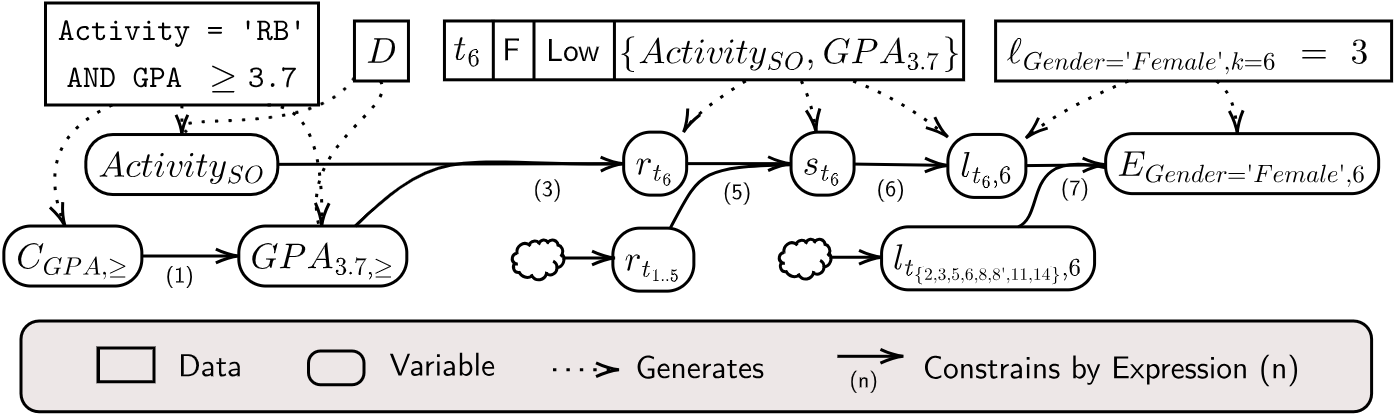
\includegraphics[width=\linewidth]{figures/example_summary.png}
    \caption{\revc{Diagram illustrating the expression generation for our running example. The predicate {\tt Activity = `RB' AND GPA $\geq$ 3.7} generates the variables $Activity_{SO}$ and $GPA_{3.7, \geq}$ as `SO' and $3.7$ are values that appear for those attributes respectively in the database $D$. $C_{GPA, \geq}$ is also generated by the predicate to hold the new constant of the predicate, and constrains the value of $GPA_{3.7, \geq}$ by (\ref{eq:value_bounds_inline}). The tuple $t_6\in \widetilde{Q}$ generates the variable $r_6$, whose value is constrained through (\ref{eq:tuple_in_ranking_inline}) by the values of $Activity_{SO}$ and $GPA_{3.7, \geq}$ due to its lineage. It also generates the variable $s_6$, which is then constrained by the value of the $r_t$ values for the tuples that rank better than it, i.e., $r_{t_{1..5}}$, through (\ref{eq:position_in_ranking_inline}). Finally, the constraint $\lb{Gender=`Female'}{k=6} = 3$ combines with $t_6$ to generate the variable $l_{t_{6},6}$ which is constrained by the value of $s_{t_6}$ by (\ref{eq:in_prefix_inline}). The constraint generates the variable $E_{Gender=`Female',6}$ which is constrained through (\ref{eq:tuples_to_satisfy_inline}) by the values of all the $l_{t, 6}$ variables for which $t$ is a part of the group (listed in \Cref{ex:deviation}).}}
    \label{fig:example_summary}
    \vspace{-0.5cm}
\end{figure}

%%%%%%%%%

% \subsection{Assignments}
% After constructing the instance of the MILP problem corresponding to the inputs of \problem{}, we use an existing MILP solver to produce an assignment $\alpha$ to the variables such that all expressions are satisfied. 
% % \yuval{Demonstrate using an example instead of the following. If possible, use the examples along the section}
% \begin{example}
%     \felix{splitting up}
    
%    % The variables $C_{Activity, RB} = 1$, $C_{Activity, SO} = 1$, $C_{GPA, \geq} = 3.7$ admit a feasible solution of our MILP model when refining the \running{} over the database shown in \Cref{ex:running}. Therefore, the set of constants for the refined predicate over $Activity$ is $\{RB, SO\}$. The refined constant of the lower-bound predicate on {\tt GPA} is then $C_{GPA, \geq}$, which is $3.7$. The refined query is finally
%    %  \begin{center}
%    %  \begin{small}
%    %  \begin{tabular}{l}
%    %      \verb"SELECT * "\\
%    %      \verb"FROM Students NATURAL JOIN Activities"\\
%    %      \verb"WHERE Gpa >= 3.7 AND (Activity = 'RB' OR Activity = 'SO')"\\
%    %      \verb"ORDER BY Sat DESC"\\
%    %  \end{tabular}
%    %  \end{small}
%    %  \end{center}
% \end{example}

%%%%%%%%%%%%%%%%%%%%%%%%%

\paragraph*{\revmulti{Model limitation}}
\label{sec:query_class_lims}
\revmulti{Given an input to our program, we construct a MILP program. The correctness of the solution generated by the program, as stated in \Cref{thm:bounded-deviation}, relies on three properties. First, every possible refinement may be represented as an assignment to the variables of the program. Second, the tuples in the output of any potential refinement are in the same relative order, and finally, every tuple in the output satisfies all the predicates of the corresponding refinement. We define the problem for SPJ queries, and thus, our model is designed to handle SPJ queries, and these properties hold for them. We note that supporting other classes of queries may require modifications to the problem definition as well as to our proposed model. For instance, in union queries, it is enough for a tuple in the output to satisfy the predicates of one branch of the union, in contrast to the third property. This may be handled straightforwardly, as noted in \Cref{sec:background}. Handling nested queries is more challenging since they may contain multiple selection statements at different nesting levels. The problem definition should first be extended to properly define how such a query can be refined, e.g., whether refinements at different nesting levels are allowed. Our proposed model cannot capture the refinement of selection statements in different nesting levels and, therefore, does not fulfill the first property. Moreover, if the {\tt ORDER BY} clause relates to an inner query, refining the inner query may change the relative order of the tuples in contrast to the second property.}


% In our presented model, these properties holds for SPJ queries but may be broken for other classes of queries. For instance, our model nested queries may not fulfill the first and second property as our model can not capture all possible refinements and


% It is important to note that the correctness of \Cref{thm:bounded-deviation} relies on some assumptions about the input query $Q$. We assume that $\widetilde{Q}$ is a query that retrieves all tuples that may be selected by any possible refinement, that the tuples in the output of any possible refinement are in the same relative order as in the output of $\widetilde{Q}$, and that a tuple fulfills all the predicates of the refinement. The first and second assumptions may be broken by a query that has subqueries: removing the predicates of the subquery and the parent query will not necessarily result in a query retrieving all possible tuples, and if the subquery is used as part of the {\tt ORDER BY} expression, refining it may change the relative order of tuples between refinements. The final assumption may be violated by a query with a union, where a tuple needs only to fulfill the predicates of one branch of the union. These assumptions are, however, fulfilled by SPJ queries, thereby motivating the limiting assumption made in \Cref{sec:background}. We note that our model may be extended to richer classes of queries if these assumptions are treated appropriately for these classes. 


% \paragraph*{\revmulti{Assumptions for correctness}}
% \label{sec:query_class_lims}
% \revmulti{It is important to note that the correctness of \Cref{thm:bounded-deviation} relies on some assumptions about the input query $Q$. We assume that $\widetilde{Q}$ is a query that retrieves all tuples that may be selected by any possible refinement, that the tuples in the output of any possible refinement are in the same relative order as in the output of $\widetilde{Q}$, and that a tuple fulfills all the predicates of the refinement. The first and second assumptions may be broken by a query that has subqueries: removing the predicates of the subquery and the parent query will not necessarily result in a query retrieving all possible tuples, and if the subquery is used as part of the {\tt ORDER BY} expression, refining it may change the relative order of tuples between refinements. The final assumption may be violated by a query with a union, where a tuple needs only to fulfill the predicates of one branch of the union. These assumptions are, however, fulfilled by SPJ queries, thereby motivating the limiting assumption made in \Cref{sec:background}. We note that our model may be extended to richer classes of queries if these assumptions are treated appropriately for these classes.} 

% \indent Recall that we obtain the lineage annotations for all tuples that may be returned by a possible refinement by evaluating $\widetilde{Q}$ over the database. However, consider a query $Q$ containing a subquery with selection predicates. Then, computing $\widetilde{Q}$ would not necessarily result in all the possible tuples. By removing the selection predicates from both the parent query and subquery, we get the set of tuples evaluated for that particular subquery rather than all the possible refined subqueries. Expression (\ref{eq:position_in_ranking_inline}) assumes that the relative orders between tuples are consistent between refinements in order to determine the position of the tuple in the output. If the subquery were used as part of the {\tt ORDER BY} clause, then it is possible that modifying the predicates of the subquery could change the relative order of the tuples between refinements. Expression (\ref{eq:tuple_in_ranking_inline}) assumes that a tuple must fulfill all the predicates of the query in order to be in its output. However, if $Q$ has a union such that $Q = Q_1 \cup Q_2$, then a tuple needs to only fulfill the predicates of (i.e. have its lineage included in) either $Q_1$ or $Q_2$.\\
% \indent These assumptions currently limit us to supporting SPJ queries, for which these assumptions are true: $\widetilde{Q}$ will return all possible tuples, the relative ordering of tuples between refinements remains consistent, and all predicates must be fulfilled in order for a tuple to be in the output. However, our approach is amenable to be extended to richer classes of queries, and in fact the extension to union is straightforward.}


%%%%%%%%%%%%%%%%%%%%%%%%%%%%%%%%%%%%%%%%%%%%%%%%%%%%%%

\section{Optimizations}
\label{sec:optimizations}
In Section~\ref{sec:search}, we have presented a MILP formulation designed to solve the \problem{} problem. While this approach enables us to leverage existing MILP solvers, that can solve the problem efficiently, they often encounter difficulties when dealing with extensive programs (containing numerous expressions), and a large number of variables~\cite{QFix}. While the number of expressions and variables in the MILP we generate is linear in the data size, as we show in Section~\ref{sec:experiments}, MILP solvers struggle to scale and solve the generated programs.


% , and struggle to scale (pointer to experiments). \yuval{can we say something about the number of expressions we generate?} 

To this end, we propose three optimizations for the construction of the MILP problem: one is a general optimization that applies in all cases, and the other two are limited in some cases. The first optimization is relevancy-based and removes from consideration tuples that are irrelevant to determining the satisfaction of the constraint set. The second optimization reduces the number of binary variables in the MILP problem by combining redundant variables. This optimization cannot be applied for queries with a {\tt DISTINCT} statement. %for queries without {\tt DISTINCT} statements.
The third optimization relaxes the expression used to determine the score of a tuple in the new ranking. This optimization is only applicable to tuples belonging to groups with only lower-bound or only upper-bound constraints, but not both.

%%%%%%%%%

\paragraph*{Relevancy-Based}
We propose a relevancy-based optimization to reduce the number of expressions and variables in our problem.
% to the mixed integer linear program in \Cref{fig:milp}, in order to reduce the number of expressions and variables in our problem. %It is noted in~\cite{QFix} that the performance of MILP solvers is in particular sensitive to these parameters. 
Recall that we use $k^*$ to denote the maximal $k$ that appears in the constraint set $\constraints$. Then, by removing tuples that could never appear in the top-$k^*$ in any refinement, we are able to avoid adding their variables and expressions to our problem. We determine the relevancy of these tuples by selecting the top-$k^*$ of the groups of tuples that share the same lineage. Let $[\prov(t)]$ be the equivalence class of tuples that share the same lineage as a tuple $t$. Then for a tuple $t$, let $T(t)$ be the ranking generated by ranking the tuples of $[\prov(t)]$ according to the {\tt ORDER BY} clause of $Q$. We see trivially that it is not possible for tuples past position $k^*$ in $T(t)$ for all $t$ in $\widetilde{Q}(D)$ to be included in the top-$k^*$ of any refinement. Thus, it is sufficient to consider only the top-$k^*$ of $T(t)$, denoted by $T(t)_{k^*}$, in the generated program, and we replace $\widetilde{Q}(D)$ in the expressions referencing it with $T(t)_{k^*}$ in Figure~\ref{fig:milp}. 


% We then substitute $\widetilde{Q}(D)$ in the expressions referencing it with the ranking generated by $\bigcup_{t \in \widetilde{Q}(D)} T(t)_{k^*}$ ranked according to the {\tt ORDER BY} of $Q$.

% \indent We define $k^*$ as the length of the maximal prefix of the constraint set $\constraints$. Then, by removing tuples that could never appear in the top-$k^*$ in any refinement, we are able to avoid adding their variables and inequalities to our problem. We determine the relevancy of these tuples by selecting the top-$k^*$ of the groups of tuples that share the same lineage. Let $[\prov(t)]$ be the equivalence class of tuples that share the same lineage as a tuple $t$. Then, let $T$ be the ranking of $[\prov(t)]$ according to the {\tt ORDER BY} clause of $Q$. We see trivially that it is not possible for tuples past position $k^*$ in $T$ to be included in the top-$k^*$ of any refinement. We then substitute $\widetilde{Q}(D)$ with $\bigcup_{t \in \widetilde{Q}(D)} T_{k^*}$ ranked according to the {\tt ORDER BY} of $Q$ in all definitions of our inequalities.
\begin{example}\label{ex:optimization1}
    % Continuing from our running example, consider the tuple $t_{14}$ with $\prov(t_{14}) = \{Activity_{RB}, GPA_{3.7}\}$.
    %\yuval{The lineage is defined with respect to the query. This is not the lineage of the tuple in the running example}. 
    Consider $t_{14}$ from Table~\ref{tab:joined}. Its equivalence class $[\prov(t_{14})]$ is the set $\{t_7, t_{10}, t_{14}\}$. Assume we are interested in satisfying a single constraint $\lb{Gender=`Female'}{2} = 1$. Note that the tuple $t_{14}$ can never appear in the top-$2$ of any refinement query, as any refinement that includes $t_{14}$ includes tuples with its same lineage, i.e., $t_7$ and $t_{10}$. Therefore, it is safe to remove all variables and expressions related to $t_{14}$ from consideration.
    % Then, the equivalence class $[\prov(t_{14})]$ is the set $\{t_7, t_{10}, t_{14}\}$. For simplicity, consider instead a singleton constraint set with a smaller maximum prefix: $\lb{Gender=`Female'}{2} = 1$. The deviation from the constraint then depends only on the top $2$ tuples. Now, notice that the tuple $t_{14}$ may never appear in the top-2, as any refinement that includes $t_{14}$ includes tuples with its same lineage, i.e., $t_7$ and $t_{10}$. The tuples $t_7$ and $t_{10}$ rank better than $t_{14}$, meaning that $t_{14}$ can never be in the top-$2$. Therefore, it is safe to remove $t_{14}$ from consideration. 
\end{example}
This optimization is most effective when $k^*$ is small, and there are few lineage equivalence classes. In \Cref{sec:experiments}, we show that this is often the case in queries over real data sets. We further demonstrate the effect of $k^*$ on the running time in \Cref{fig:time_vs_k}.

% this in \Cref{fig:time_vs_k}, which shows that the running time of the algorithm increases with $k^*$.

%%%%%%%%%

\paragraph*{Selecting Lineages} 
% The next optimization leverages the notion of lineage equivalence classes to reduce the number of variables. 
Recall that the program we generate includes a binary variable $r_t$ for each tuple in $\widetilde{Q}(D)$. However, tuples sharing the same lineage all have equal values for their $r_t$ variables. Therefore, we can use a single variable for all tuples in the same lineage equivalence classes. 

% The idea is to use a single variable for all tuples with the same lineage instead of their $r_t$ variables, as they all share the same assignment. 
% We propose another optimization to reduce the number of variables constructed in the MILP problem by using this notion of lineage equivalence classes to select all the tuples of a selected lineage with one variable, instead of constructing variables for tuples individually. \\
% \indent Our original construction of the MILP problem creates a binary variable $r_t$ for each tuple in $\widetilde{Q}(D)$. However, tuples sharing the same lineage all have equal values for their $r_t$ variables. Therefore, many of these variables are redundant and could share one variable made for the tuples of its lineage instead.
\begin{example}
    To demonstrate this idea, consider the \running{} without its {\tt DISTINCT} statement and consider again the tuple $t_{14}$ with its equivalence class shown in Example~\ref{ex:optimization1}. If $t_{14}$ satisfies the selection condition of a refinement on the \running{}, then $t_7$ and $t_{10}$ must satisfy the conditions as well, as they share the same lineage. Therefore, we have the equivalence $r_{t_{14}} = r_{t_7} = r_{t_{10}}$. The variables $r_{t_7}$ and $r_{t_{10}}$ are then made redundant, as they always have the same value as $r_{t_{14}}$. 
\end{example}

In order to avoid such redundancy, instead of constructing the set of $r_t$ variables, we construct a set of variables $r_{[\prov(t)]}$ for every tuple $t$ in $\widetilde{Q}(D)$. Using (\ref{eq:tuple_in_ranking_inline}) as a basis, we are able to model $r_{[\prov(t)]}$ being assigned $1$ if and only if the tuples in $[\prov(t)]$ satisfy the selection condition of the corresponding refinement query.
% the lineage is selected.
 Instead of constructing expression (\ref{eq:tuple_in_ranking_inline}) for each tuple in $\widetilde{Q}(D)$, we construct the following expression for each $r_{[\prov(t)]}$ variable:
% \begin{align*}
    $0 \leq \sum_{p \in \prov(t)} p - |\conds(Q)| \cdot r_{[\prov(t)]} \leq |\conds(Q)| - 1$.
% \end{align*}
Furthermore, in order to ensure that the $s_t$ values are modeled as before, we modify (\ref{eq:position_in_ranking_inline}) by changing $r_t$ to $r_{[\prov(t)]}$ and $r_{t'}$ to $r_{[\prov(t')]}$.
We note that this optimization cannot be applied if the input query includes a {\tt DISTINCT} statement,
% However, we cannot use this optimization where the input query has a {\tt DISTINCT} statement,
as we need this information in order to not select tuples that already have a tuple sharing its distinct value selected.
%%%%%%%%%

\begin{table*}[t!]
    \centering
    \footnotesize  
    % \hspace*{-0.5cm}
    \begin{tabular}{lclcl}
    \hline
    \textbf{Dataset} & \textbf{Query} & \multicolumn{1}{c}{\textbf{Predicates}} & \textbf{Order by (DESC)} & \multicolumn{1}{c}{\textbf{Constraints}}\\ \hline\hline
    Astronauts & $Q_A$ & 
    \begin{tabular}{l@{}}\texttt{"Graduate Major" = 'Physics'}\\ \texttt{AND "Space Walks" <= 3}\\ \texttt{AND "Space Walks" >= 1} \end{tabular}  
    &{\tt "Space Flight (hrs)"}&\begin{tabular}{@{}ll@{}}
        (1) $\lb{Gender='F'}{k} = \frac{k}{2}$ & (4) $\lb{Status='Management'}{k} = \frac{k}{5}$ \\ (2) $\lb{Gender='M'}{k} = \frac{k}{2}$ & (5) $\lb{Status='Retired'}{k} = \frac{k}{5}$ \\ (3) $\lb{Status='Active'}{k} = \frac{k}{5}$ &
    \end{tabular}\\
    \hline
    Law Students & $Q_L$ & \begin{tabular}{l@{}}\texttt{Region = 'GL'}\\\texttt{AND GPA <= 4.0}\\\texttt{AND GPA >= 3.5}\end{tabular}& {\tt LSAT}&\begin{tabular}{@{}ll@{}}
        (1) $\lb{Sex='F'}{k} = \frac{k}{2}$ & (4) $\lb{Race='White'}{k} = \frac{k}{5}$ \\ (2) $\lb{Sex='M'}{k} = \frac{k}{2}$ & (5) $\lb{Race='Asian'}{k} = \frac{k}{5}$ \\ (3) $\lb{Race='Black'}{k} = \frac{k}{5}$ &
    \end{tabular}\\
   \hline
    MEPS & $Q_M$ & \begin{tabular}{l@{}}\texttt{Age > 22}\\\texttt{AND "Family Size" >= 4}\end{tabular}& {\tt Utilization}&\begin{tabular}{@{}ll@{}}
        (1) $\lb{Sex='F'}{k} = \frac{k}{2}$ & (4) $\lb{Race='Black'}{k} = \frac{k}{5}$ \\ (2) $\lb{Sex='M'}{k} = \frac{k}{2}$ & (5) $\lb{Race='White'}{k} = \frac{k}{5}$ \\ (3) $\lb{Race='Asian'}{k} = \frac{k}{5}$ &
    \end{tabular}\\ \hline
    TPC-H & $Q_5$ & \texttt{Region = 'ASIA'} & {\tt Revenue}& \begin{tabular}{@{}ll@{}}
        (1) $\lb{OrderPrio='5-LOW'}{k} = \frac{k}{2}$ & (4) $\lb{MktSeg='BUILDING'}{k} = \frac{k}{5}$ \\ (2) $\lb{OrderPrio='3-MEDIUM'}{k} = \frac{k}{5}$ & (5) $\lb{MktSeg='MACHINERY'}{k} = \frac{k}{5}$ \\ (3) $\lb{MktSeg='AUTOMOBILE'}{k} = \frac{k}{5}$ &
    \end{tabular}\\ \hline
    \end{tabular}
    \caption{Queries and constraints}
    \label{tab:queriesAndConstraints}
    \vspace{-0.5cm}
\end{table*}

\paragraph*{Relaxation for Single-Constraint-Type Tuples}
%\yuval{this part is still not clear}
We present another optimization that is possible when a tuple belongs to groups that have only either lower-bound ($\ell$) or upper-bound ($\mathscr{u}$) cardinality constraints made on them. We define the set of tuples belonging only to groups with lower-bound constraints as 
% $$L = \{ t \mid \not\exists (\ub{G, k} = n) \in \constraints, t \in \sigma_G(\widetilde{Q}(D)) \}$$
$L = \{ t \mid \not\exists (\ub{G}{k} = n) \in \constraints, t \in \widetilde{Q}(D) \cap G \}$.
We define a similar set $U$ for upper-bound tuples, replacing $\ub{G}{k} = n$ in the quantifier with $\lb{G}{k} = n$. Then, for a tuple $t \in L$, we relax expression (\ref{eq:position_in_ranking_inline}) to 
$1 + |\widetilde{Q}(D)| \cdot (1 - r_t) + \sum_{t' \in \widetilde{Q}(D), \widetilde{Q}(D)(t') < \widetilde{Q}(D)(t)} r_{t'} \leq s_{t}$.
% We may relax tuples in $U$ similarly by specifying an upper bound instead. 

For tuples in $U$ we use an upper bound instead ($\geq s_t$). This relaxation makes finding feasible solutions for this model easier and may be used by presolving techniques in MILP solvers.
% 
To understand why this maintains the correctness of our solution, consider the lower-bound constraints. Intuitively, we can allow the $s_t$ variables of tuples belonging to the group defined in the constraint in a given top-$k$ to be assigned a value larger than the position of $t$ in the ranking, as this can only result in a worse deviation from satisfying the constraint (but can not assign a value smaller than the position of $t$ in the ranking). The case for upper-bound constraints is symmetric.




% "leave" it (i.e. assign $s_t$ a value larger than the position of $t$ in the ranking), as this can only result in a worse deviation from satisfying the constraint. However, we cannot have the tuples belonging to this group outside of that prefix "enter" it (i.e. assign $s_t$ a value smaller than the position of $t$ in the ranking), as this might result in claiming a lower deviation than reality. The case for upper-bound constraints is symmetric.

% \begin{example}
%     Consider the assignment feasible for (\ref{eq:value_bounds_inline}-\ref{eq:position_in_ranking_inline}) corresponding to the original \running{}. Let $t_{14}$ be the tuple corresponding to student \#14 in \Cref{tab:candidates} joined with \Cref{tab:internships} (shown in \Cref{tab:joined}). In the ranking $R$ generated by the query, we have $R(t_{14}) = 7$. Therefore, we have $s_{t_{14}} = 7$. However, by making the relaxation as seen above, we instead have $s_{t_{14}} \geq 7$, meaning that this tuple can not be used to count towards satisfying the cardinality constraint $\lb{Gender='Female'}{6} = 3$.
% \end{example}

% \section{Experiments}
\label{sec:experiments}

This section evaluates the algorithm of Section~\ref{sec:solution} on real data.
All results below were produced on the real UCI Adult extract ($N=48{,}842$) and the real Tax benchmark ($N=500{,}000$).

\subsection{Experimental Goals}
\label{subsec:experimental-goals}

\begin{description}
  \item[RQ1 -- Use cases.] Do the released explanations identify the semantic change a refinement actually makes, on the query pairs the paper motivates?
  \item[RQ2 -- Scalability.] How does running time depend on $k$, $N$, $\epsilon$, $|\mathcal{P}|$, $\tau$, $\gamma$, and on the choice of algorithm?
  \item[RQ3 -- Quality.] How close is the private algorithm to non-private references, measured against three separate baselines?
\end{description}

\subsection{Experimental Setup}
\label{subsec:experimental-setup}

\subsubsection{Datasets and Query Pairs}
\label{subsubsec:datasets}

\paragraph{Adult.} The real UCI Adult extract, $48{,}842$ records.
We use two refinements, denoted Adult 6.7 (occupation broadening) and Adult 6.8 (education--hours), listed in Table~\ref{tab:query-pairs}.

\paragraph{Tax.} The real Tax benchmark used in the data-cleaning literature, $500{,}000$ records, with the marital-status refinement denoted Tax 6.6 in Table~\ref{tab:query-pairs}.

\paragraph{Not evaluated.}
IPUMS-CPS and the Stack Overflow Developer Survey are not included in this pass, and the Hospital/CQA setting is not evaluated at all: the framework has only ever been exercised on query-refinement pairs, never on a repair-semantics pair, and doing so would additionally require implementing repair semantics.
Section~\ref{sec:usecase-results} therefore substantiates the query-refinement use case only.

\begin{table}[t]
\centering
\small
\caption{Query pairs, on the real data. Each $Q$ violates its representation constraint and each $Q'$ satisfies it.}
\label{tab:query-pairs}
\begin{tabular}{@{}llrrr@{}}
\toprule
Pair & Constraint & $|Q|$ & $|Q'|$ & share in $Q\rightarrow Q'$ \\
\midrule
Adult 6.7  & $\ge25\%$ female   & 5{,}447  & 37{,}155  & $4.7\%\rightarrow26.9\%$ \\
Adult 6.8  & $\ge25\%$ female   & 3{,}055  & 2{,}453   & $19.5\%\rightarrow30.6\%$ \\
Tax 6.6    & $\ge30\%$ HasChild & 145{,}576 & 291{,}659 & $3.5\%\rightarrow50.1\%$ \\
\bottomrule
\end{tabular}
\end{table}

The Adult 6.8 figures reproduce the numbers quoted in Section~\ref{sec:introduction} ($19.5\%\rightarrow30.6\%$) exactly, on the real data.

\subsubsection{Parameters}
\label{subsubsec:parameters}

Unless stated otherwise $k=5$, $\lambda=0.5$, $\epsilon=1$, and the budget is split equally, $(\epsilon_P,\epsilon_S,\epsilon_H)=(\epsilon/3,\epsilon/3,\epsilon/3)$; $\tau$ and $\gamma$ follow Eqs.~\eqref{eq:tau-rule} and~\eqref{eq:gamma-rule}, giving $\tau=15$ and $\gamma\approx150$ on both datasets.
Equal shares is not an arbitrary default: sweeping the split over the three query pairs found no allocation that dominates it.
Equal shares gave the lowest released-histogram error on all three, and the best selection quality on the hardest of them.
Starving the view stage is the one clearly bad choice, since the explanation stage can only choose among the views that survive it: at $(0.10,0.55,0.35)$ the approximation ratio on Adult education-hours falls from $0.89$ to $0.57$.
Moving budget the other way buys a few points of selection quality on that pair alone and costs histogram accuracy on all three.
\alon{TODO: all numbers below were produced with $\tau=35$ and $\gamma=\lceil0.005N\rceil$ ($244$ for Adult, $2{,}500$ for Tax). They must be re-run under Eqs.~(\ref{eq:tau-rule}) and~(\ref{eq:gamma-rule}), \added{and now also under Eq.~(\ref{eq:gammaR-rule}), $\gamma_R=N/100$ in place of $\gamma_R=N$, with the view-stage sensitivity $\Delta=4/|D|$ of Proposition~\ref{prop:usefulness-sensitivity} in place of $7/(4|D|)$}. A first look on Adult education-hours, scored against a fixed yardstick so the comparison does not move with $\gamma$, put the new setting ahead of the old one, so the rerun is expected to improve rather than weaken the results.}
\alon{TODO (experiment to add): measure the view stage in isolation. For each query pair and each $\epsilon_P$, report the overlap between the privately retained $\tau$ views and the exact top-$\tau$ by $\Use$, and the lowest $\Use$ actually retained against the true $\tau$-th best. A first look at Adult education-hours suggests the overlap is low at the budgets used here and rises sharply with $\epsilon_P$, which would explain why the view stage is the one that must not be starved (Section~\ref{subsubsec:parameters}) and would give Section~\ref{subsec:two-stages} the empirical counterpart to the utility guarantee it lacks.}

Reported quantities average $40$ trials; this count is not incidental, as the between-trial standard deviation of set score is frequently comparable to its mean, and smaller counts cannot separate configurations reliably.

\subsection{Compared Methods}
\label{subsec:compared-methods}

We compare the algorithm of Section~\ref{sec:solution} against three baselines.

\begin{description}
  \item[B1 --- $\epsilon\rightarrow\infty$.] The identical algorithm, run with a privacy budget large enough that every mechanism is numerically deterministic. Isolates the cost of privacy noise alone, holding the architecture fixed.
  \item[B2 --- exhaustive optimum, non-private.] Enumerates \emph{all} size-$k$ subsets of the candidate explanations, scores each with the set-level objective of Definition~\ref{def:setobj}, and returns the maximiser.
  \item[B3 --- greedy, non-private.] Takes the top-$\tau$ views by $Usefulness$ with no privacy mechanism, then performs $k$ rounds selecting the best remaining histogram with no privacy mechanism.
\end{description}

B2 is exponential in $k$: with $\tau=35$ views and $10$ attributes the candidate space holds $350$ explanations and $\binom{350}{5}\approx5\times10^{11}$ subsets, which is not enumerable.
It is nevertheless computed \emph{exactly}, by restricting the search to the union over attributes of the top-$k$ candidates of each attribute group.
That restriction is lossless: if an optimal set contained a candidate outside the top-$k$ of its own group, some higher-scoring member of that group would be unused, and swapping it in cannot decrease $F_\lambda$, which is non-decreasing in the score of every member.
The pool is therefore $k\,|Attrs|=50$ candidates and $\binom{50}{5}\approx2.1\times10^{6}$ subsets, and B2 is the true optimum of the $\tau$-filtered space rather than an approximation to it.

\paragraph{Scoring.}
All four methods are scored on their output \emph{set} under one common yardstick: the paper's own objective, Definition~\ref{def:hd} with $\gamma_{\text{eval}}=0$, combined with the set-level utility of Definition~\ref{def:setobj}.
This is deliberate. Smoothing is a mechanism-internal device, and allowing it to define the metric as well would make the comparison circular; scoring at $\gamma_{\text{eval}}=0$ means the algorithm is judged by the standard of the unmodified paper even though it selects under smoothing.

\subsection{Use Case Results}
\label{sec:usecase-results}

\begin{figure}[t]
\centering
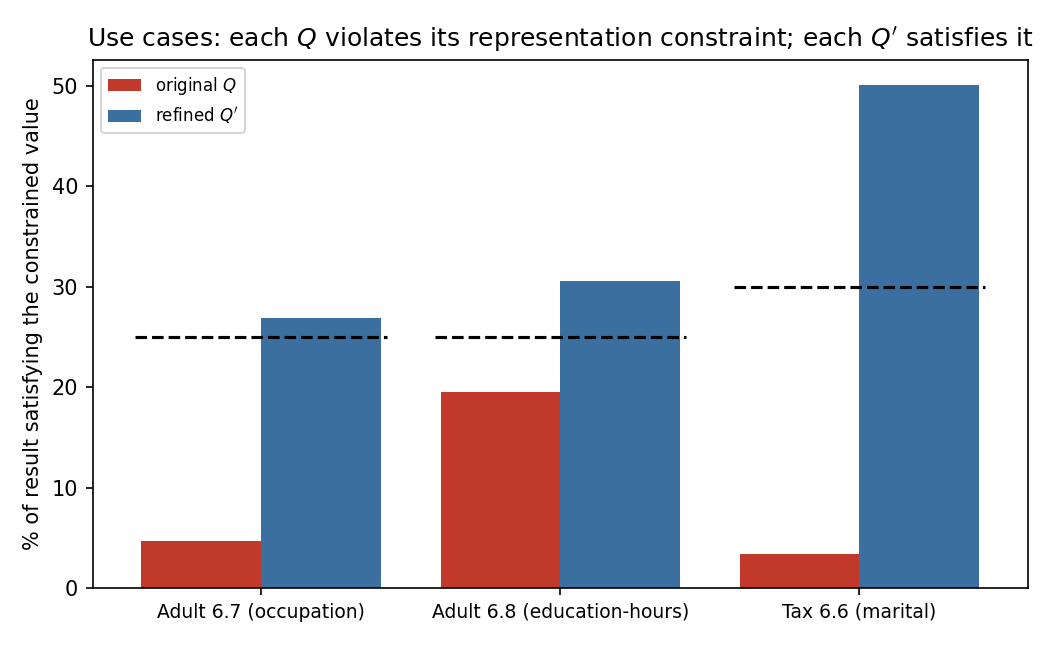
\includegraphics[width=\linewidth]{figures/U1_constraint_premise.png}
\caption{Each original query violates its representation constraint (dashed line) and each refined query satisfies it, on the real data.}
\label{fig:premise}
\end{figure}

Figure~\ref{fig:premise} establishes the premise: on real data all three refinements do what the motivating examples claim.
Figures~\ref{fig:rel-tax}--\ref{fig:rel-adult-edu} show the differentially private explanations the algorithm releases for each pair at $\epsilon=1$, $k=5$.

\begin{figure}[t]
\centering
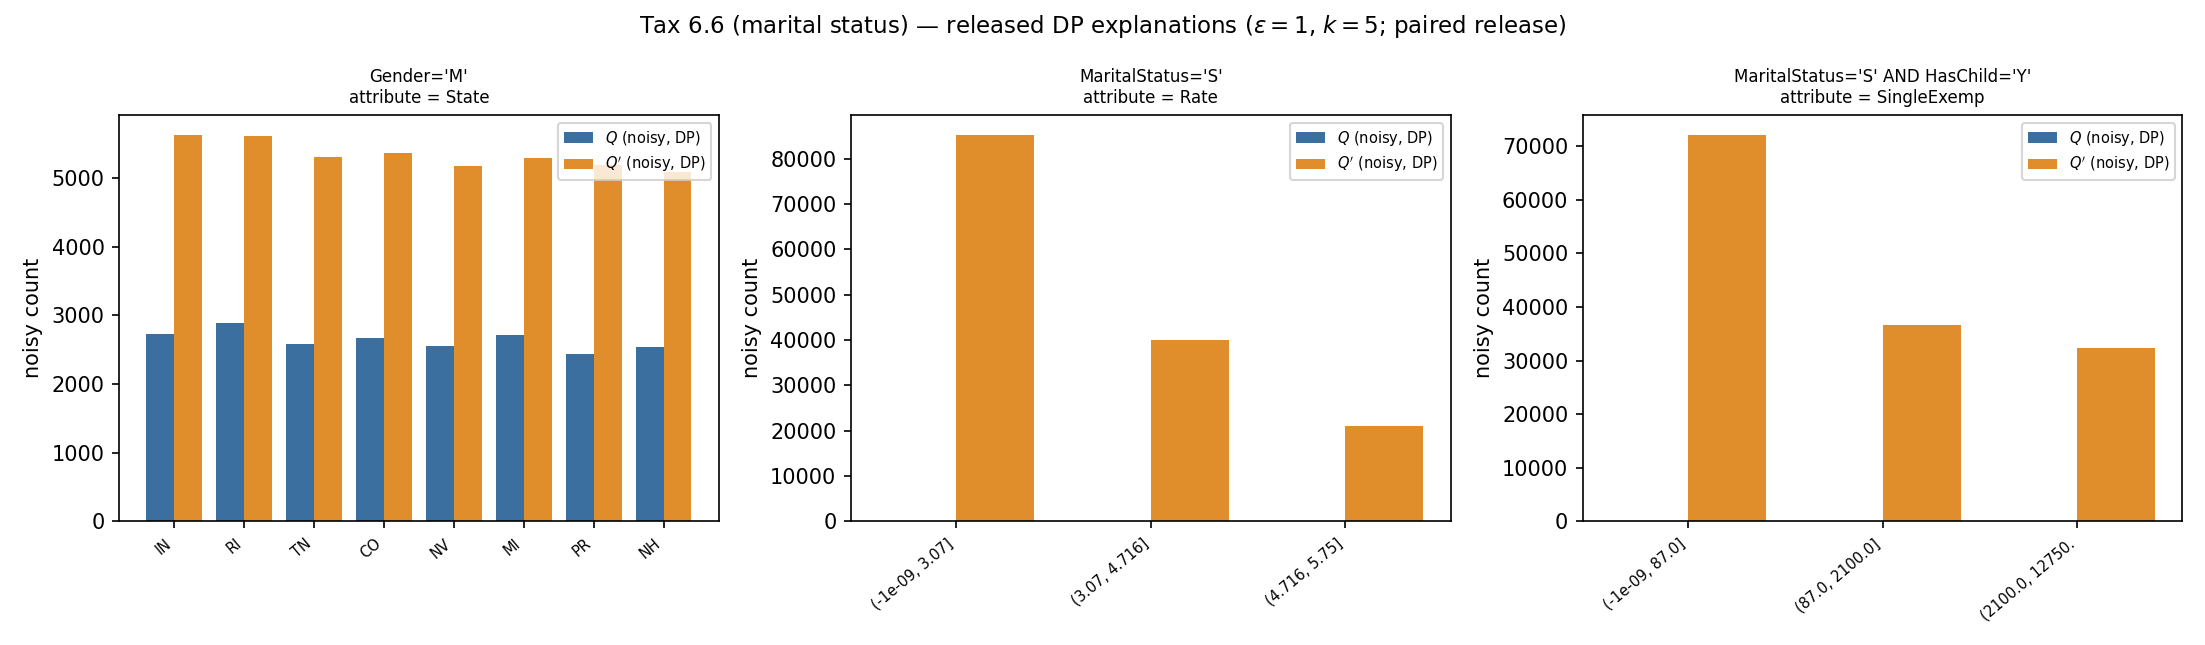
\includegraphics[width=\linewidth]{figures/U2_released_tax_marital.png}
\caption{Tax 6.6 --- released differentially private explanations.}
\label{fig:rel-tax}
\end{figure}

For Tax the refinement removes the predicate $\texttt{MaritalStatus}=\texttt{'M'}$.
The algorithm recovers exactly that subgroup: three of the five released explanations are conditioned on $\texttt{MaritalStatus}=\texttt{'S'}$, the population the refinement mechanically introduces, with a shift of $-85{,}178$ tuples concentrated in the lowest \texttt{Rate} bucket.
The framework is never given the query predicates.

\begin{figure}[t]
\centering
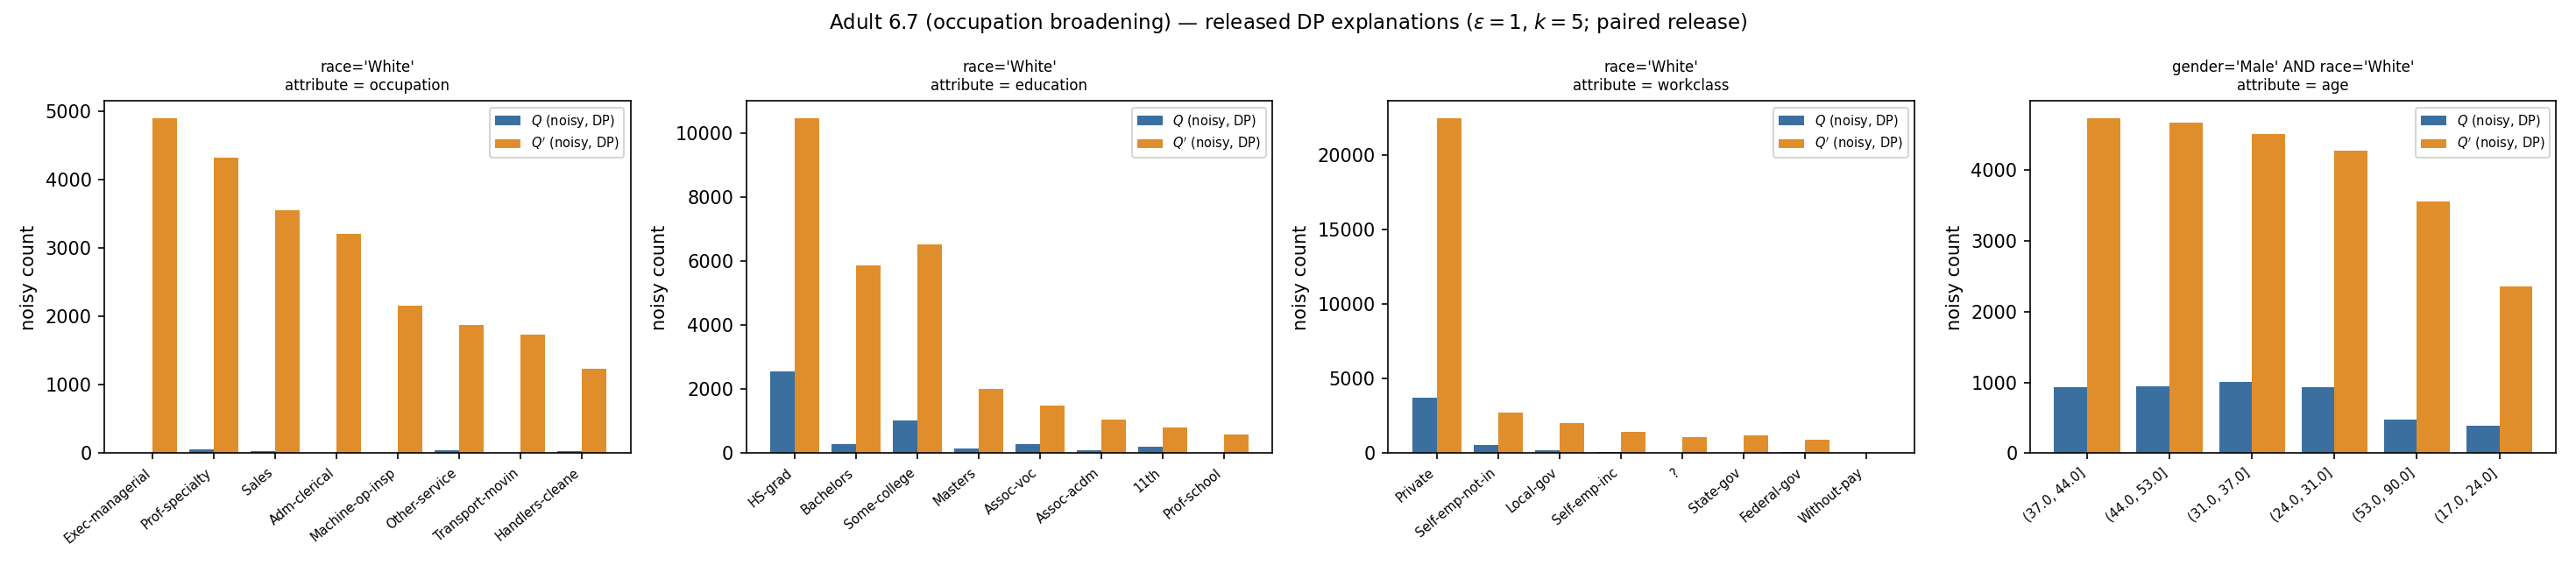
\includegraphics[width=\linewidth]{figures/U2_released_adult_occupation.png}
\caption{Adult 6.7 --- released differentially private explanations.}
\label{fig:rel-adult-occ}
\end{figure}

\begin{figure}[t]
\centering
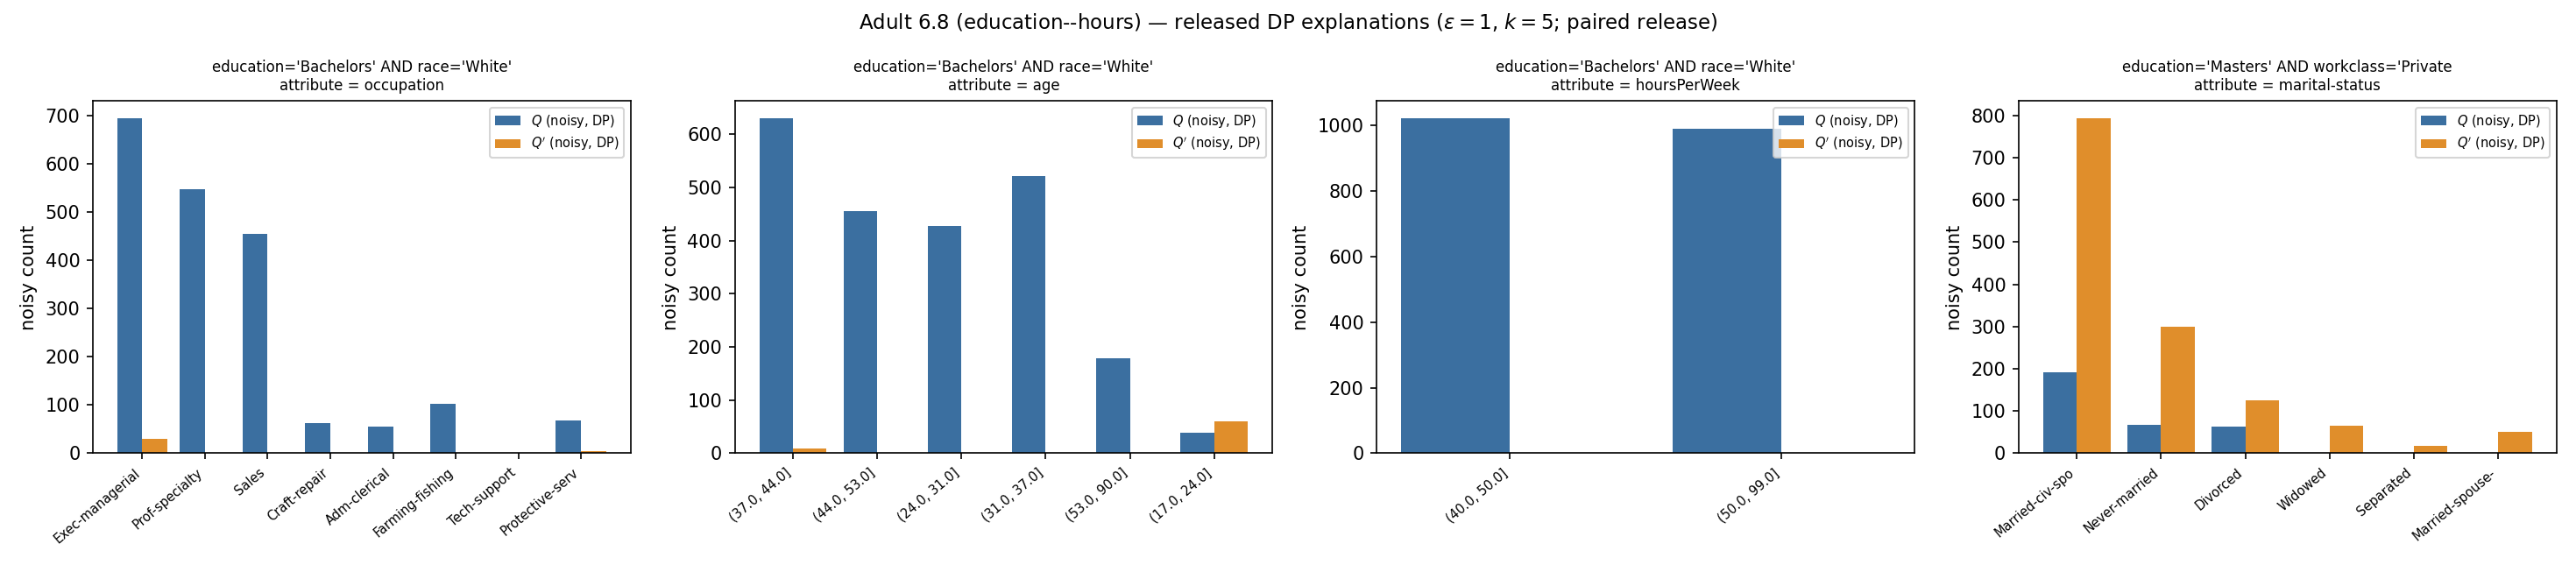
\includegraphics[width=\linewidth]{figures/U2_released_adult_education_hours.png}
\caption{Adult 6.8 --- released differentially private explanations.}
\label{fig:rel-adult-edu}
\end{figure}

For Adult 6.7 the released explanations are dominated by shifts \emph{within} $\texttt{race}=\texttt{'White'}$ across \texttt{occupation}, \texttt{education} and \texttt{workclass}, showing that broadening a narrow occupational query changes the occupational and educational composition of the result rather than merely enlarging it.
For Adult 6.8 the explanations localise on $\texttt{education}=\texttt{'Bachelors'}$ subgroups, which is the population the refinement removes when it restricts education to \texttt{Masters}.

These are the un-cherry-picked outputs of a single run at the default parameters.

\subsection{Scalability}
\label{subsec:scalability}

\begin{figure*}[t]
\centering
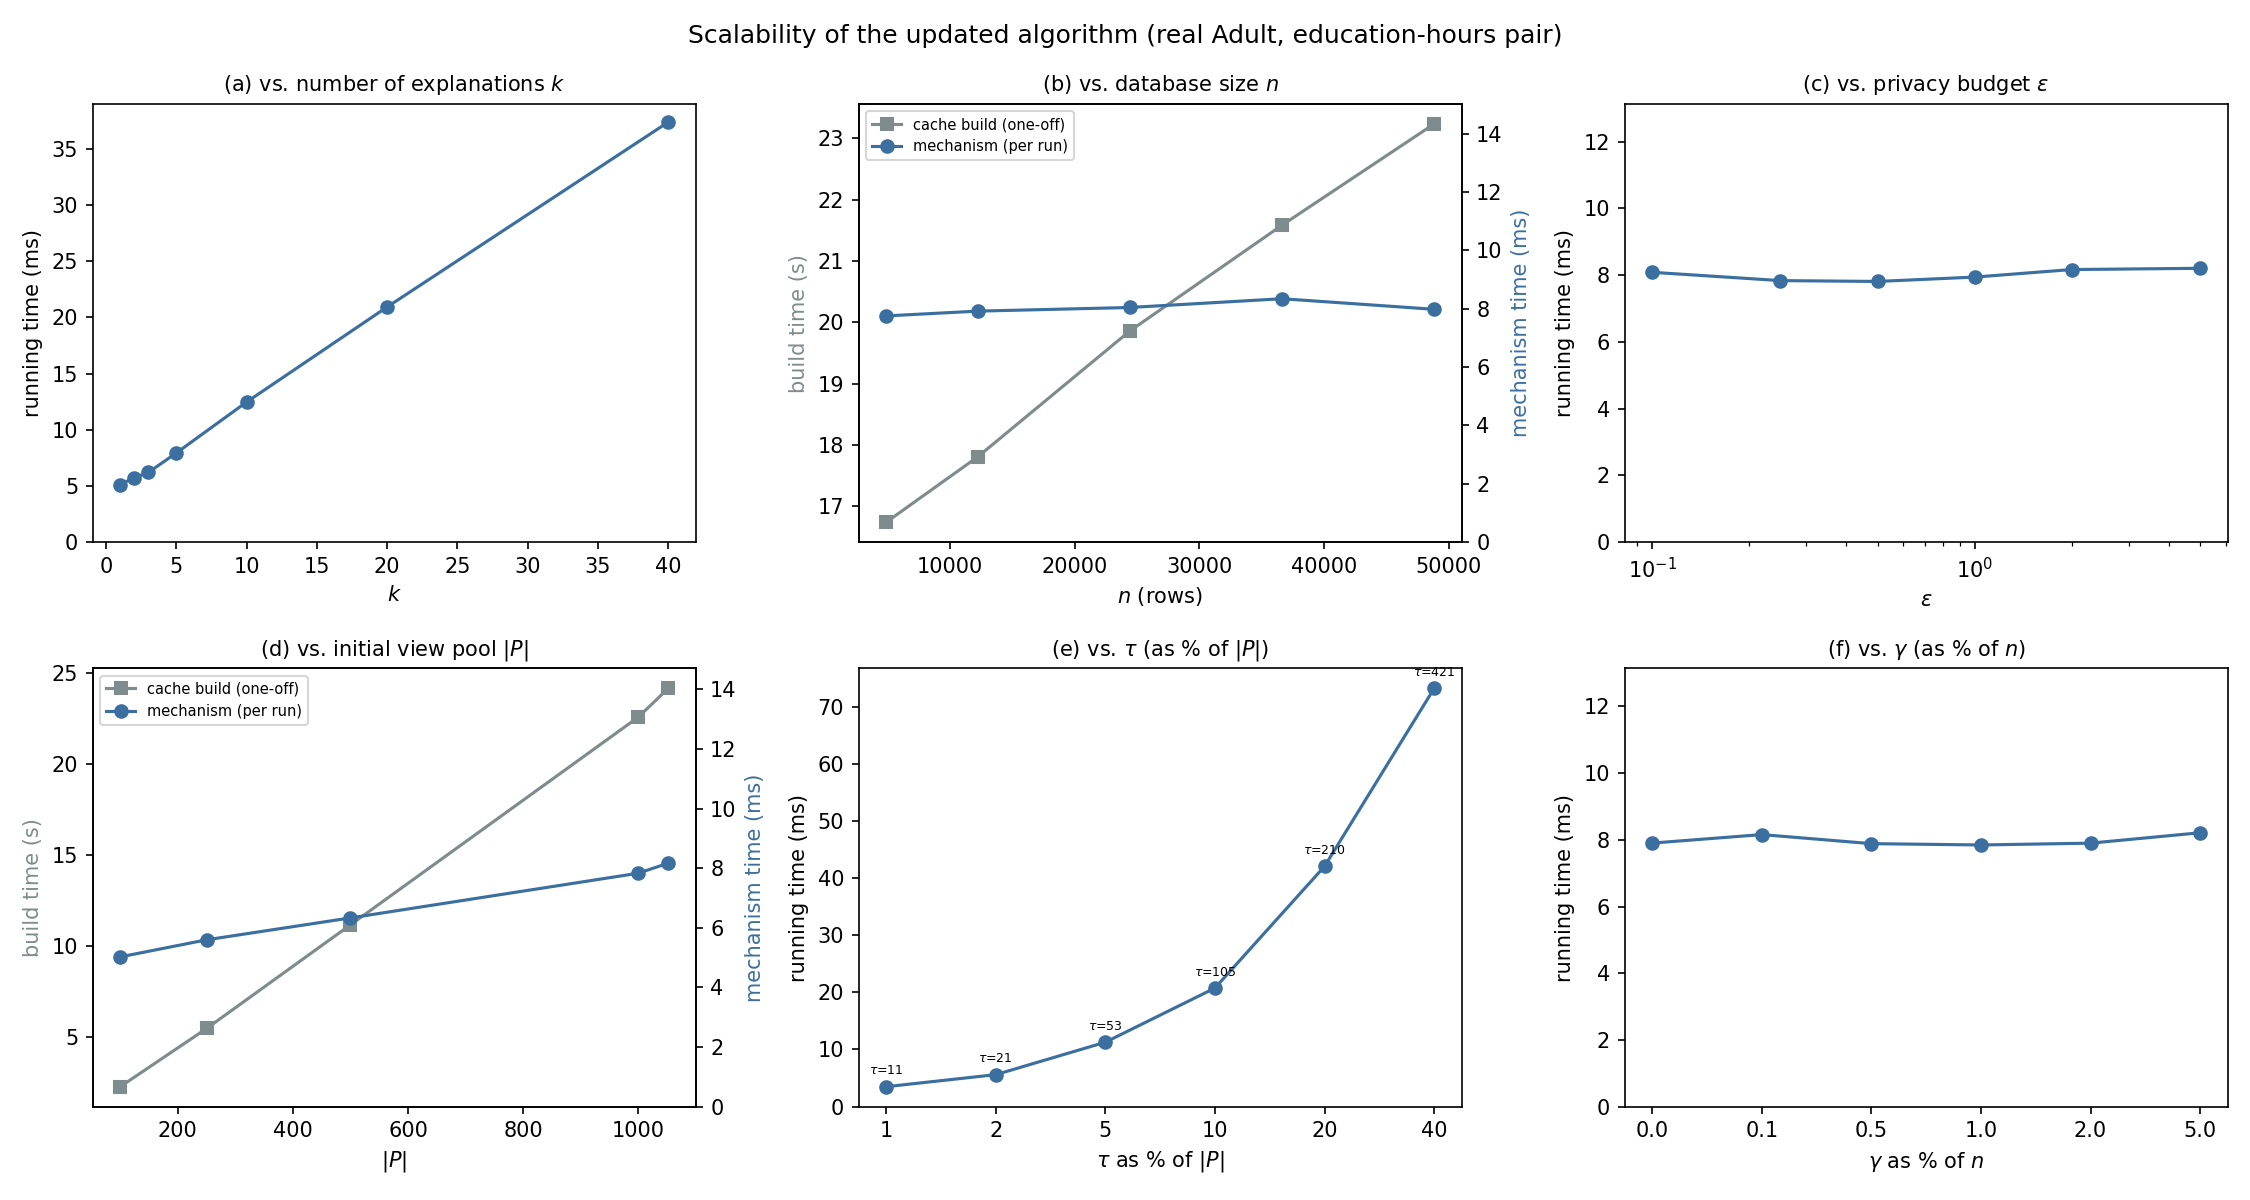
\includegraphics[width=\linewidth]{figures/S1_scalability_grid.png}
\caption{Running time of the algorithm. Panels (b) and (d) separate the one-off cache build, which carries the $O(N)$ and $O(|\mathcal{P}|)$ work, from the per-invocation mechanism cost.}
\label{fig:scalability}
\end{figure*}

Figure~\ref{fig:scalability} reports the six sweeps.

\paragraph{$k$, $\tau$, $|\mathcal{P}|$.}
Running time is linear in $k$ ($4.6$\,ms at $k=1$ to $36.3$\,ms at $k=40$) and in $\tau$, matching the $O(k\tau m b)$ term of Section~\ref{subsec:complexity-analysis}.
Expressed as a fraction of $|\mathcal{P}|$, moving $\tau$ from $5\%$ to $10\%$ doubles per-round cost ($11.1$\,ms to $19.9$\,ms) and from $5\%$ to $40\%$ multiplies it sevenfold.

\paragraph{$N$ and $|\mathcal{P}|$.}
The per-invocation cost is essentially flat in $N$ ($7.7$--$8.3$\,ms across a tenfold range), because the $O(N)$ work is confined to the one-off preprocessing, which grows from $16.7$\,s to $23.2$\,s over the same range.
Panels (b) and (d) plot both; presenting only the per-run curve on an autoscaled axis would turn a sub-millisecond spread into an apparent trend.

\paragraph{$\epsilon$ and $\gamma$.}
Running time is invariant to both ($7.8$--$8.2$\,ms across $\epsilon\in[0.1,5]$, and $7.9$--$8.3$\,ms across $\gamma$ from $0\%$ to $5\%$ of $N$).
For $\epsilon$ this is the expected result and confirms no budget-dependent overhead.
For $\gamma$ it is a consequence of the caching described in Section~\ref{subsec:complexity-analysis}: $\gamma$ enters only the denominator, so changing it costs nothing.
This is what makes re-scoring at a different $\gamma$ free in running time as well as in privacy.

\subsubsection{Running Time by Algorithm}
\label{subsec:runtime-algorithm}

\begin{figure}[t]
\centering
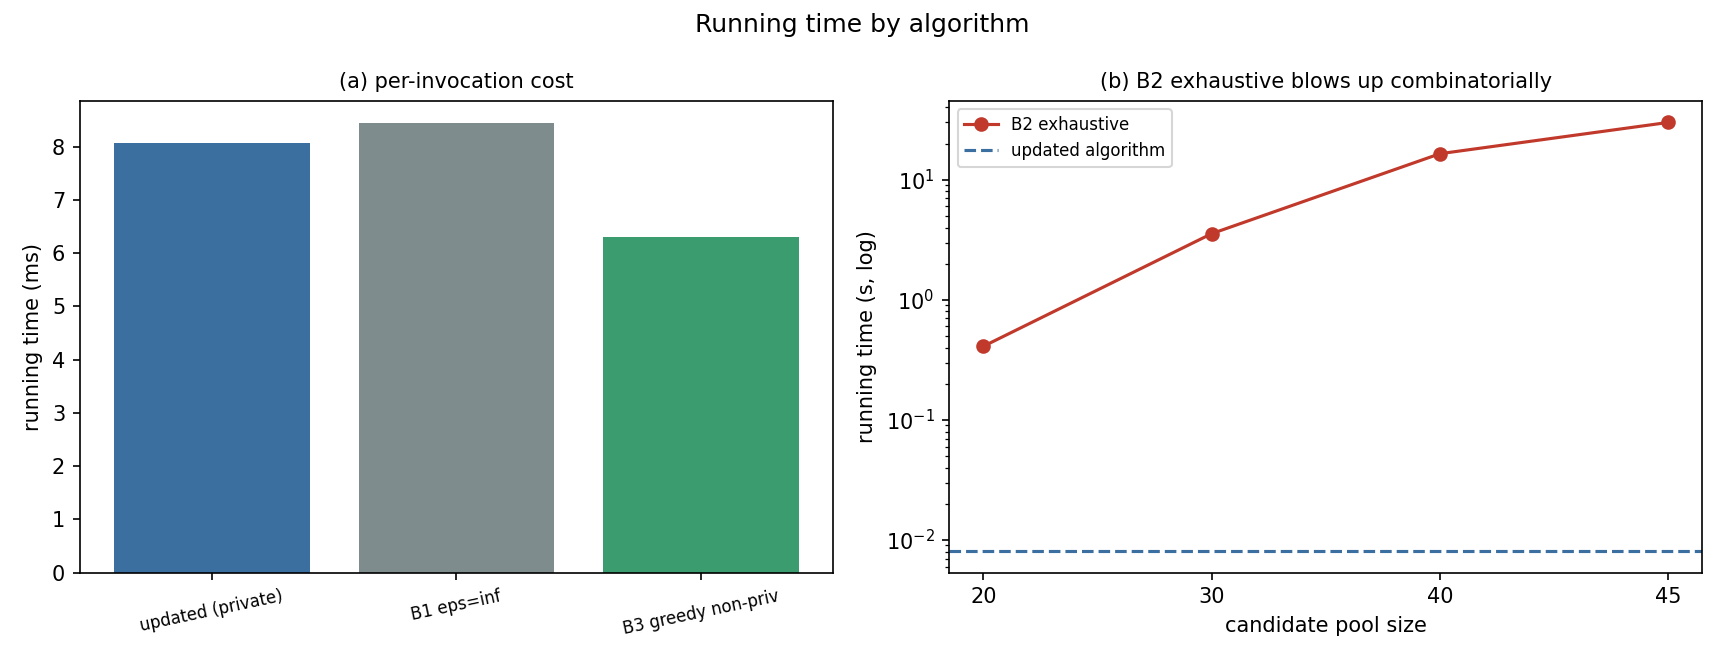
\includegraphics[width=\linewidth]{figures/S2_runtime_by_algorithm.png}
\caption{Per-invocation cost of each method, and the combinatorial blow-up of the exhaustive baseline B2.}
\label{fig:runtime-algorithm}
\end{figure}

The private algorithm ($8.1$\,ms), B1 ($8.4$\,ms) and B3 ($6.3$\,ms) are all within a small constant of one another: privacy costs essentially nothing in running time, since the exponential mechanism replaces an $\arg\max$ over the same scores.

B2 is different in kind.
On a $20$-candidate pool it takes $0.41$\,s; at $30$, $3.6$\,s; at $40$, $16.5$\,s; at $45$, $30.0$\,s --- a $73\times$ increase for a $2.25\times$ increase in pool size, tracking $\binom{|C|}{5}$.
On the lossless $50$-candidate pool it takes $57$\,s, versus $8$\,ms for the private algorithm.
Enumerating the unrestricted $350$-candidate space would take on the order of months, which is why the losslessness argument above is needed rather than optional, and why the selection is run greedily: by Proposition~\ref{prop:greedy-exact} that costs nothing in quality.

\subsection{Quality}
\label{subsec:quality}

\begin{figure*}[t]
\centering
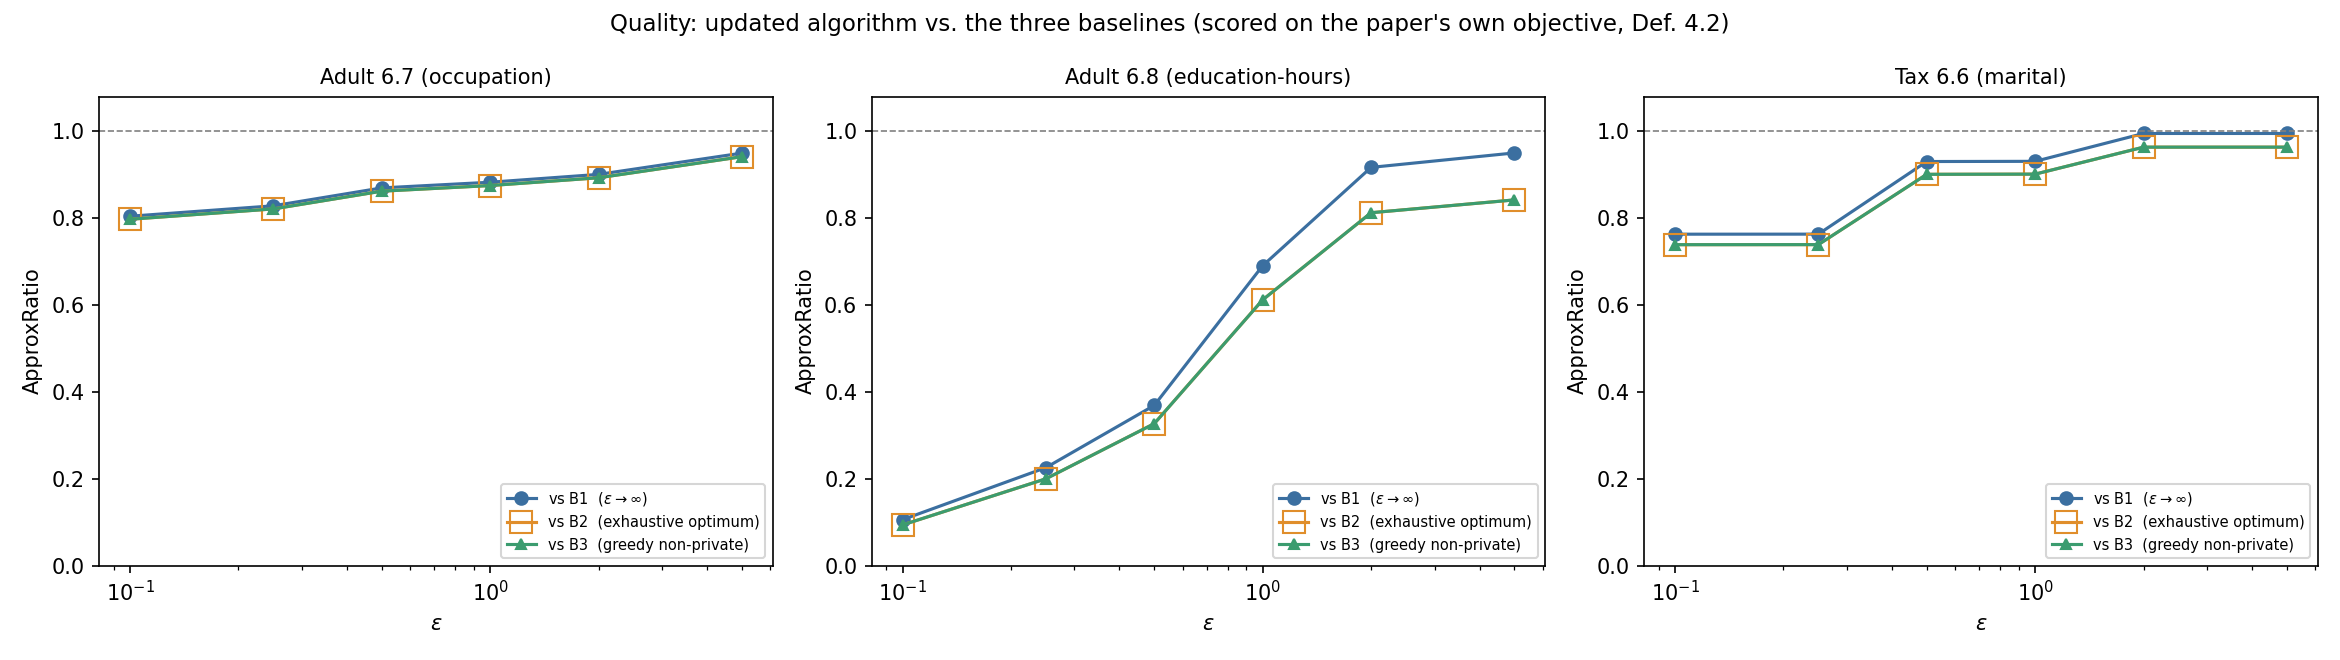
\includegraphics[width=\linewidth]{figures/Q1_approxratio_vs_baselines.png}
\caption{ApproxRatio of the algorithm against each baseline, scored on the paper's own objective ($\gamma_{\text{eval}}=0$), $40$ trials per point.}
\label{fig:quality}
\end{figure*}

\begin{table}[t]
\centering
\small
\caption{ApproxRatio against each baseline at $\epsilon=1$ and $\epsilon=5$.}
\label{tab:quality}
\begin{tabular}{@{}lcccccc@{}}
\toprule
& \multicolumn{3}{c}{$\epsilon=1$} & \multicolumn{3}{c}{$\epsilon=5$}\\
\cmidrule(lr){2-4}\cmidrule(lr){5-7}
Pair & B1 & B2 & B3 & B1 & B2 & B3\\
\midrule
Adult 6.7 & 0.883 & 0.875 & 0.875 & 0.950 & 0.941 & 0.941\\
Adult 6.8 & 0.691 & 0.612 & 0.612 & 0.950 & 0.842 & 0.842\\
Tax 6.6   & 0.931 & 0.901 & 0.901 & 0.995 & 0.963 & 0.963\\
\bottomrule
\end{tabular}
\end{table}

At the default $\epsilon=1$ the algorithm attains $0.88$--$0.93$ of the $\epsilon\rightarrow\infty$ reference on two of the three pairs and $0.88$--$0.90$ of the exhaustive optimum, rising to $0.94$--$1.00$ and $0.94$--$0.96$ respectively at $\epsilon=5$.
Adult 6.8 is the hardest pair and the only one that degrades sharply at small $\epsilon$ ($0.11$ against B1 at $\epsilon=0.1$); it is also the pair whose top candidates are most tightly bunched, so the exponential mechanism has the least separation to exploit.

Two observations are worth isolating.

First, \textbf{B2 and B3 coincide exactly on all three query pairs} (Figure~\ref{fig:absolute}): the non-private greedy procedure attains the true optimum of the $\tau$-filtered space, not merely an approximation to it.
This is what Proposition~\ref{prop:greedy-exact} predicts: on a fixed candidate set and a fixed $\gamma$ greedy returns the exact maximiser, so the two references answer the same question here.
The measurement confirms it on real instances rather than establishing it.

Second, the ratio against B2/B3 is consistently slightly below the ratio against B1.
B1 holds the architecture fixed and removes only the noise, so it isolates the cost of privacy; B2/B3 remove the noise \emph{and} search without a privacy-imposed $\tau$ budget, so the residual gap to them also includes what the mechanism gives up by having to select views privately at all.
Reporting both separates those two costs.

\begin{figure}[t]
\centering
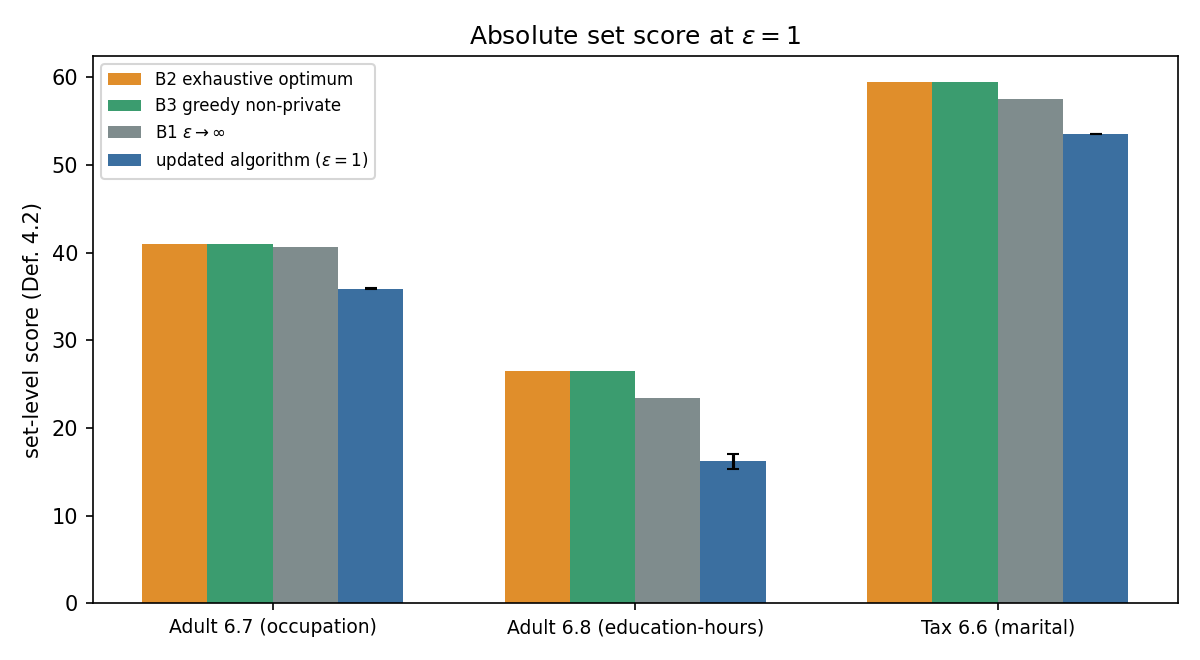
\includegraphics[width=\linewidth]{figures/Q2_absolute_scores.png}
\caption{Absolute set scores at $\epsilon=1$. B2 and B3 coincide exactly: non-private greedy attains the exhaustive optimum on every pair.}
\label{fig:absolute}
\end{figure}

\subsubsection{The $\gamma$ Trade-off}
\label{subsec:gamma-tradeoff}

Smoothing is not free, and the cost is worth stating precisely.
$\gamma$ competes against the size of individual histogram \emph{bins}, and the bin-count distribution relative to $|D|$ differs sharply between datasets: the median non-empty bin holds $20$ tuples on Adult but $3{,}897$ on Tax, a factor of $200$ despite only a factor of $10$ in $N$.
Consequently the same "fraction of $N$" rule lands in very different regimes.
At $\gamma=0.5\%$ of $N$, $\gamma$ exceeds the bin count for $84\%$ of Adult bins but only $30\%$ of Tax bins; at $5\%$ of $N$ it exceeds $98\%$ and $94\%$ respectively, at which point the median ratio $m_v/(m_v+\gamma)$ falls to $0.008$ on Adult and $HD_\gamma$ has effectively stopped measuring \emph{relative} change at all.

The pre-registered rule of Section~\ref{subsubsec:parameters} is therefore defensible but crude, and $\gamma$ at $5\%$ of $N$ would be clearly too aggressive.
A sharper anchor follows from Proposition~\ref{prop:hd-sensitivity}: the separation available to the exponential mechanism scales as $\epsilon\,\delta u\,(1+\gamma)/2$, so the $\gamma$ actually required is governed by the \emph{margin} between the leading candidates rather than by $N$.
Measured on the three pairs, that margin is $0.027$, $0.121$ and $0.315$ respectively, implying required $\gamma$ of roughly $292$, $66$ and $25$ --- an ordering unrelated to dataset size, and inverted with respect to it.

\subsection{Summary of Findings}
\label{subsec:experiments-summary}

Running time is linear in $k$, $\tau$ and $|\mathcal{P}|$, invariant to $\epsilon$ and $\gamma$, and independent of $N$ once preprocessing is amortised; privacy adds no measurable cost relative to the non-private greedy baseline, while the exhaustive baseline is intractable beyond a few dozen candidates.
On quality the algorithm reaches $0.88$--$0.93$ of the $\epsilon\rightarrow\infty$ reference at the default budget and $0.95$--$1.00$ at $\epsilon=5$, judged by the paper's own unsmoothed objective; non-private greedy attains the exhaustive optimum exactly on all three pairs, as Proposition~\ref{prop:greedy-exact} predicts.
The use cases show that the released explanations localise the population a refinement adds or removes without being given the query predicates --- most sharply on Tax, where three of five released explanations recover exactly the subgroup the dropped predicate introduces.
The principal caveat is the choice of $\gamma$: it is what makes private selection work at these budgets, but anchoring it to a fraction of $|D|$ is a crude proxy for the quantity that actually determines it.


% \section{Related Work}
\label{sec:related}

We discuss three lines of work: how the pair of query outputs that we explain is produced, how existing systems explain query results and differences between data, and how differential privacy has been used for explanations. To our knowledge, no prior work generates differentially private explanations for the differences between two related query outputs.

\emph{Query refinement and repair.}
Query refinement has been studied for queries with empty answers~\cite{muslea2005online,KoudasLTV06} and for queries that must meet constraints on the size of the output~\cite{MK09,chu1994structured}.
Recent work refines queries to satisfy diversity and representation constraints.
Erica~\cite{ERICA,LMSJ23} changes a query so that the result meets constraints on the sizes of several subgroups. It uses provenance annotations to do this efficiently.
The work in~\cite{SSAD22} finds a fair query that is close to the user's query. It supports range predicates and a binary sensitive attribute.
The work in~\cite{CSSM24} changes the selection conditions of top-$k$ queries.
Provenance has also been used to analyze and reduce bias in data-driven tools~\cite{MLJ22}.
In consistent query answering, queries are evaluated over the repairs of an inconsistent database~\cite{arenas1999,bertossi2006,bertossi2011}.
These systems return a refined query or a repaired answer. They give limited support for explaining what the change means for the data.
Our framework treats the process that produces the second output as a black box, so it can be used together with these systems (Section~\ref{subsec:prelim-settings}).

\emph{Explaining query results and data.}
Provenance~\cite{buneman2001,cheney2009,herschel2017} tracks why and where output data comes from.
Intervention-based work~\cite{RoyS14} explains an aggregate result with predicates that select tuples whose removal changes the result.
Scorpion~\cite{wu2013} finds predicates that explain outliers in aggregate results using properties of the input tuples.
Why-not questions~\cite{CJ09,tran2010conquer} ask why some tuples are missing from a query result.
CAPE~\cite{MZGR19} explains an outlier in an aggregate result by values that deviate in the opposite direction.
MacroBase~\cite{MacroBase} explains outliers with attribute-value combinations that are common among outliers and rare among inliers. It ranks them with the relative risk ratio.
DIFF~\cite{DIFF} is a relational operator that provides the functionality of such explanation engines.
Some works are closer to ours.
SeeDB~\cite{SeeDB} scores a view by the distance between its distributions on a target subset and on a reference subset.
FEDEX~\cite{FEDEX} scores a data exploration step by how much it changes the distribution of an attribute.
Contrast set mining~\cite{BayPazzani01} and emerging patterns~\cite{DongLi99} look for conjunctions of attribute values whose distribution or support differs between groups or datasets.
We use the interestingness, coverage, representativeness and diversity measures from this literature (Section~\ref{subsec:prelim-quality}).
However, these works mainly explain a single query result, a prediction, or a data transformation. They do not explain the differences between two related query outputs.
In addition, explanations based on individual tuples cannot be used under differential privacy~\cite{TaoGMR22}.

\emph{Differential privacy for explanations.}
DPXPlain~\cite{TaoGMR22} explains aggregate query results under differential privacy.
The user compares the aggregate values of two groups in a query result.
DPXPlain releases noisy answers, a confidence interval for the difference between the groups, and a table of top-$k$ explanation predicates.
The predicates are selected with the one-shot top-$k$ mechanism~\cite{DurfeeRogers19}.
DPClustX~\cite{DPClustX} explains clustering results under differential privacy using histograms. It works in two stages.
It replaces quality measures with high sensitivity by measures with low sensitivity.
Like both works, we use private selection. Like DPClustX, we release noisy histograms and use quality measures with low sensitivity.
Our setting is different. We explain the difference between two related query outputs, such as a query and its refinement.
Our quality measures are defined for this comparison (Section~\ref{sec:explanation-quality}).
Each explanation is a pair of noisy histograms of an attribute inside a selected view.
Systems for differentially private data analysis~\cite{mcsherry2009,JNS18,JNHS20} support aggregate queries. As noted in~\cite{TaoGMR22}, private SQL systems do not support explanations.
We build our algorithms from known mechanisms: the exponential mechanism~\cite{mcsherry2007}, one-shot top-$k$~\cite{DurfeeRogers19} and the Laplace mechanism~\cite{DMNS2006}.
We smooth the denominators of ratio-based scores to bound their sensitivity. A similar idea is used in differentially private decision trees~\cite{FriedmanSchuster10} and in~\cite{DPClustX}.

% \section{Conclusion}
\label{sec:conclusion}

We identified a novel intervention to diversify (according to user-input constraints) the output of top-$k$ queries by refining the selection predicates of the input query. Furthermore, we recognized the importance of maintaining the user's intent as best as possible when searching for such a refinement. Towards this end, we developed a framework that can find the closest refinement for various distance measures that satisfy the user's desired constraints. 
%We based our solution on the notion of {\it lineage} from the provenance literature, which we combined with mixed-integer linear programming to efficiently find the best approximation refinement in an otherwise large search space. 
We introduced optimizations in order to make our framework practical for datasets of real-life scale. We demonstrated this with a suite of experiments, showing our framework's scaling capability and the usefulness of our optimizations. In the future, this problem could be extended to find refinements that remain diverse even after adding new data. This way, the refinement may explain some underlying bias of the query instead of fitting to the original data. \revmulti{Extending our model to richer classes of queries presents further interesting directions as we discussed in \Cref{sec:search}.} 
% Extension to union is straightforward as noted in \Cref{sec:background}, while extension to subqueries would prove more challenging. Such an extension would need to treat the fact that making refinements to the predicates of the subqueries may change the relative order of the tuples.}

% that this type of intervention is reasonably effective.
% \subsubsection*{Future work}
% \felix{13/10 draft}
% While the refinements made by our framework work with the existing data, ideally the refinement should maintain a similar level of deviation from the set of constraints as new data is added. Were this the case, it means that the refinement made identified some underlying bias in the query, rather than fitting it to the existing data. We believe that this framework could be extended to produce refinements that are robust to new data in attempt to better capture any underlying biases.

% \resolve{Until here (October -- draft)} 
% {\color{red}\hrule}

% \felix{no acks?}
% \begin{acks}
%  This work was supported by the [...] Research Fund of [...] (Number [...]). Additional funding was provided by [...] and [...]. We also thank [...] for contributing [...].
% \end{acks}

\bibliographystyle{ACM-Reference-Format}
\bibliography{sections/bibliography}
\section{Exact Greedy Selection}
\label{app:greedy}

\begin{proposition}[The rounds are exact greedy]
\label{prop:greedy-exact}
Fix a candidate set $\mathcal{E}'\subseteq\mathcal{E}$ and a smoothing constant $\gamma$, and let $w_j=\lambda^{\,j-1}$.
\begin{enumerate}[label=(\roman*),leftmargin=*]
\item The score $\HD_\gamma(p,A)\cdot\lambda^{Counts[A]}$ that line~4 of Algorithm~\ref{alg:topk} assigns a remaining candidate is exactly its marginal gain in $F_w$, so selecting the highest-scoring candidate is one step of greedy on $F_w$.
\item For any non-increasing $w$, selecting $E\subseteq\mathcal{E}'$ with $|E|=k$ maximising $F_w(E)$ is solvable in polynomial time, and greedy returns an optimal solution.
\end{enumerate}
\end{proposition}

\begin{proof}
(i) In a given round all candidates carrying an attribute $A$ share the factor $\lambda^{Counts[A]}$, so whenever a round selects from that group it selects the member of largest $\HD_\gamma$; after $c$ selections from $A$ the members taken are therefore its $c$ highest-scoring ones.
Every remaining candidate of $A$ thus scores no higher than any already taken, so adding it places it at rank $c+1$ of its group and leaves the ranks of the existing members unchanged.
The group term of Eq.~\eqref{eq:set-objective} gains exactly $w_{c+1}h=\lambda^{c}h$, which is the score of line~4, and no other group term changes.

(ii) By Definition~\ref{def:setobj}, $F_w(E)=\sum_A g_A(E)$ where $g_A$ depends only on the members of $E$ whose attribute is $A$.
There is therefore no interaction between groups, and a solution is determined by how many candidates $n_A\ge0$ it takes from each group, subject to $\sum_A n_A=k$, together with which ones.
For a fixed $n_A$, the best choice within group $A$ is its $n_A$ highest-scoring candidates, since $w$ is non-increasing and the scores are ranked (rearrangement inequality).
Hence the value of taking $g$ candidates from group $A$ is
\[
f_A(g)=\sum_{j=1}^{g} w_j\, h^A_{(j)},
\]
whose successive marginal gains are $f_A(g)-f_A(g-1)=w_g\,h^A_{(g)}$.
These are non-increasing in $g$, because $w_g$ is non-increasing by assumption and $h^A_{(g)}$ is non-increasing by construction; so each $f_A$ is concave.

Maximising a separable sum of concave functions subject to a cardinality constraint is exactly the problem solved by the greedy rule of repeatedly taking the largest remaining marginal gain, which is optimal for separable concave resource allocation.
Since each marginal gain is computable in constant time after sorting each group, the total cost is $O(|\mathcal{E}'|\log|\mathcal{E}'|)$ for $|\mathcal{E}'|$ candidates.
With (i), the $k$ rounds of Algorithm~\ref{alg:topk} run exactly this procedure.
\end{proof}



\begin{example}[Greedy and the optimum agree]
\label{ex:greedy}
Let $\lambda=\tfrac12$ and $k=3$, and let five candidates carry the scores $9$ and $4$ on one attribute and $7$, $6$ and $2$ on another.
The marginal gains available are $9$ and $\tfrac12\cdot4=2$ in the first group, and $7$, $\tfrac12\cdot6=3$ and $\tfrac14\cdot2=0.5$ in the second.
Greedy takes $9$, then $7$, then $3$, for a total of $19$.
These are the three largest gains in the list, so no set of three candidates can do better, and enumerating all ten subsets confirms that $19$ is the optimum.
Taking the two best scores of the first group instead, $9$ and $4$, together with $7$, gives $18$: the second copy of an attribute is discounted, which is what makes the greedy order follow the discounted gains rather than the raw scores.
\end{example}


\end{document}
\endinput
